\documentclass[a4paper, 12pt, openright]{book}
\usepackage{preamble}

\usepackage{comment}
\usepackage{lipsum}
%\usepackage{booktabs}
\usepackage{array}
\usepackage{setspace}
\usepackage[osf]{newpxtext} % Palatino font
%\usepackage{newpxmath} % Palatino font
\usepackage{fmtcount} % Convert number to corresponding word

% Set lists layout
\setlist[description]{
    font={\fontfamily{zplTOsF}\itshape}
}

\renewcommand{\labelenumi}{\fontfamily{zplTOsF}\bfseries\itshape\roman{*}.}

% Suppress page numbering and header on empty pages
\makeatletter
    \def\cleardoublepage{\clearpage\if@twoside \ifodd\c@page\else
    \hbox{}
    \thispagestyle{empty}
    \newpage
    \if@twocolumn\hbox{}\newpage\fi\fi\fi}
\makeatother

% Set sizes of margins, width of text, height of header etc.
\setlength{\hoffset}{-0.5cm}
\setlength{\voffset}{-1.5cm}
\setlength{\textwidth}{38pc}
\setlength{\textheight}{55pc}
\setlength{\oddsidemargin}{3.5mm}
\setlength{\evensidemargin}{3.5mm}
\setlength{\topmargin}{7mm}
\setlength{\footskip}{40pt}
\setlength{\headheight}{14.5pt}

\AtBeginDocument{
    \setlength{\abovedisplayskip}{0.5cm}
    \setlength{\abovedisplayshortskip}{0.3cm}
    \setlength{\belowdisplayskip}{0.5cm}
    \setlength{\belowdisplayshortskip}{0.3cm}
}

% Define section format
\titleformat{\chapter}[display]{\fontfamily{zplTLF}}{\LARGE\itshape{Chapter \Numberstringnum{\thechapter}}}{1cm}{\huge\fontfamily{zplTOsF}\itshape}[]
\titlespacing{\chapter}{0pt}{50pt}{20pt}[0pt]

\titleformat{\section}[hang]{\Large\fontfamily{zplTOsF}\itshape}{\thesection}{20pt}{}

\titleformat{\subsection}[hang]{\large\fontfamily{zplTOsF}\itshape}{\thesubsection}{20pt}{}

\titleformat{\subsubsection}[hang]{\normalsize\fontfamily{zplTOsF}\itshape}{}{20pt}{}

% Define ToC format
\setcounter{tocdepth}{2} % Do not include further than subsections

\titlecontents{chapter}[0pt]{\vspace{1.0\baselineskip}\large\fontfamily{zplTOsF}\itshape}{\hyperlink{chapter.\thecontentslabel}{\thecontentslabel}\hspace*{12pt}}{}{\titlerule[0pt]\hyperlink{chapter.\thecontentslabel}{\textbf{\thecontentspage}}}[]

\titlecontents{section}[20pt]{\normalsize\fontfamily{zplTOsF}\itshape}{\hyperlink{section.\thecontentslabel}{\thecontentslabel}\hspace*{12pt}}{}{\titlerule*[0.6pc]{.}\hyperlink{section.\thecontentslabel}{\textbf{\thecontentspage}}}[]

\titlecontents{subsection}[40pt]{\normalsize\fontfamily{zplTOsF}\itshape}{\hyperlink{subsection.\thecontentslabel}{\thecontentslabel}\hspace*{12pt}}{}{\titlerule*[0.6pc]{.}\hyperlink{subsection.\thecontentslabel}{\textbf{\thecontentspage}}}[]

% Header and footer settings.
\pagestyle{fancy}
\fancyhf{} % Clear defaults
%\renewcommand{\headrule}{}
\renewcommand{\headrulewidth}{0pt}
\renewcommand{\footrulewidth}{0pt}
\renewcommand{\chaptermark}[1]{\markboth{\thechapter. #1}{}}
\renewcommand{\sectionmark}[1]{\markright{\thesection. #1}}
\fancyhead[RE]{\fontfamily{zplTOsF}\textsc{\leftmark}}
\fancyhead[LO]{\fontfamily{zplTOsF}\textsc{\rightmark}}
\fancyfoot[RO]{\fontfamily{zplTOsF}\textit{\thepage}}
\fancyfoot[LE]{\fontfamily{zplTOsF}\textit{\thepage}}

% Redefine the plain page style
\fancypagestyle{plain}{%
  \fancyhf{}%
  \fancyfoot[R]{\fontfamily{zplTOsF}\textit{\thepage}}%
  \renewcommand{\headrulewidth}{0pt}% Line at the header invisible
  \renewcommand{\footrulewidth}{0pt}% Line at the footer visible
}

% Set epigraphs style
\usepackage{epigraph}
\setlength{\epigraphrule}{0pt}
\setlength{\beforeepigraphskip}{0.5\baselineskip}
\setlength{\afterepigraphskip}{0.5\baselineskip}
\newcommand{\myepigraph}[2]{\epigraph{\textsl{``#1''}}{--- #2}}

% Set commenting commands
\newcommand{\evan}[1]{{\color{red}{EOC: #1}}}
\newcommand{\haakon}[1]{{\color{teal}{HA: #1}}}
\newcommand{\oliver}[1]{{\color{olive}{OEA: #1}}}
\newcommand{\gad}[1]{{\color{orange}{GJ: #1}}}
\newcommand{\review}[1]{{\color{brown}#1}}

% Define custom chapter
\newcommand{\mainchapter}[4]{
    \chapter{#1}
    \renewcommand{\epigraphflush}{flushright}
    \setlength{\epigraphwidth}{#2\textwidth}
    \myepigraph{#3}{#4}
    \begin{center}
        \(\star\)
    \end{center}
    \vspace{1\baselineskip}
}

% Cref setup
\creflabelformat{equation}{#2#1#3}
\crefformat{section}{\S#2#1#3}
\Crefformat{section}{\S#2#1#3}
\crefrangeformat{section}{\S\S#3#1#4-#5#2#6}
\Crefrangeformat{section}{\S\S#3#1#4-#5#2#6}

% Math shortcuts
\newcommand{\upd}[1][]{\mathrm{d}\mathrm{#1}}
\newcommand{\updvec}[1]{\mathrm{d}\boldsymbol{\mathrm{#1}}}
\newcommand{\fvec}[1]{\boldsymbol{#1}}
\newcommand{\unitvec}[1]{\boldsymbol{\hat{#1}}}
\newcommand{\nablavec}{\boldsymbol{\nabla}}
\newcommand{\deriv}[2]{\frac{\mathrm{d}#1}{\mathrm{d} \mathrm{#2}}}
\newcommand{\dpart}[2]{\frac{\partial #1}{\partial #2}}

\DeclarePairedDelimiter\abs{\lvert}{\rvert}%
\DeclarePairedDelimiter\norm{\lVert}{\rVert}%

% Swap the definition of \abs* and \norm*, so that \abs
% and \norm resizes the size of the brackets, and the 
% starred version does not.
\makeatletter
\let\oldabs\abs
\def\abs{\@ifstar{\oldabs}{\oldabs*}}
%
\let\oldnorm\norm
\def\norm{\@ifstar{\oldnorm}{\oldnorm*}}
\makeatother

\setlength{\jot}{16pt}
\newenvironment{boxedeq}[1][\linewidth]{\FrameSep=8pt\abovedisplayskip=0pt\abovedisplayshortskip=0pt\belowdisplayskip=5pt\belowdisplayshortskip=5pt
\framed\hsize=#1\leftskip=\dimexpr(\textwidth-#1)/2\relax}
{\endframed}

% Physics shortcuts
\newcommand{\sunlum}{L_{\odot}}
\newcommand{\sunrad}{R_{\odot}}
\newcommand{\sunmass}{M_{\odot}}
\newcommand{\units}[1]{\,\mathrm{#1}}
\newcommand{\punct}[1]{\,\mathrm{#1}}

\newcommand{\flash}{{\fontfamily{pcr}\selectfont FLASH}}

% Set document's metadata
\title{Long Term Simulations of Core-Collapse Supernovae with a Neutron Star Central Engine}
\author{Gaétan J.A.M. Jalin}
\date{14 August 2024}

\begin{document}
% Set document's font properties
%\renewcommand{\rmdefault}{cmr}
%\renewcommand{\sfdefault}{cmss}
%\renewcommand{\ttdefault}{cmtt}
%\renewcommand{\rmfamily}{\fontfamily{cmr}}
\renewcommand{\familydefault}{cmr}
%\renewcommand{\encodingdefault}{T1}
%\DeclareSymbolFont{letters}{OML}{cmm}{m}{it}
%\DeclareSymbolFont{operators}{OT1}{cmr}{m}{n}
%\SetSymbolFont{letters}{normal}{OML}{cmm}{m}{it}
%\DeclareSymbolFontAlphabet{\mathnormal}{letters}
%\DeclareSymbolFontAlphabet{\mathrm}{operators}
%\renewcommand{\seriesdefault}{m}
\normalfont

\begin{titlepage}
    \fontfamily{zpltosf}\selectfont
    \begin{center}
        \vspace*{0.3cm}
        {\large \textsc{Master Thesis}}\\
        \vspace{0.5\baselineskip}
        \begin{spacing}{1.9}
            {\huge Long-Term Simulations
            \break %\vspace{0.3cm}
            of Core-Collapse Supernovae with a
            \break %\vspace{0.3cm}
            Neutron Star Central Engine}
        \end{spacing}

        \vspace*{0.8cm}

        {\textit{by}}\\
        \vspace*{0.6cm}
        {\Large Gaétan J.A.M. Jalin}\\
        \vspace*{0.8cm}
        %{\textit{supervised by}}\\
        {\textit{under the supervision of}}\\
        \vspace*{0.6cm}
        {\large Evan Patrick O'Connor}\\

        \vfill
        \(\star\)
        \vfill
        
        \textit{
        The Oscar Klein Centre,\\
        Department of Astronomy,\\
        Stockholm University,\\
        AlbaNova,\\
        106 91 Stockholm,\\
        Sweden
        }

        \vspace*{0.7cm}

        {August 14, 2024}

        \vspace*{1.1cm}
        
\includegraphics[width=0.6\textwidth]{SU_large.png}

        \vspace*{0.5cm}
    \end{center}
\end{titlepage}

\clearpage
\thispagestyle{empty}

\vspace*{2cm}
\vfill

\renewcommand{\epigraphflush}{center}
\setlength{\epigraphwidth}{0.55\textwidth}
\myepigraph{This page intentionally left nonblank.}{ISO/IEC/JTC1/SC22/WG5, \fontfamily{zplTOsF}\textit{Fortran 2023}}
\vspace*{2cm}


% Reintroduce for final version
\cleardoublepage
\begin{minipage}{0.8\textwidth}
    \vspace*{5cm}
    \begin{flushright}
        {
            \fontfamily{zplTOsF}\selectfont
            \large
            \textit{To my sister,\\who truly cared about me,\\Maeva}
        }
    \end{flushright}
    \vfill
\end{minipage}
\pagestyle{empty}
\clearpage

\pagenumbering{roman}
\setcounter{page}{0}
\addtocontents{toc}{\vspace*{3cm}}
\chapter*{\hfill{\centering Abstract}\hfill}
\vspace{1.5cm}

% I probably shouldn't...
%\renewcommand{\epigraphflush}{flushright}
%\setlength{\epigraphwidth}{0.4\textwidth}
%\myepigraph{Hold on to your butts \ldots}{John Raymond Arnold, \\\textit{Jurassic Park}}

\begin{center}

Current simulations of core-collapse supernovae mainly focus on the first moments of the explosion, up to a few seconds after collapse. Such simulations come at a large computational cost and rarely extend to later times, limiting our ability to compare with observations.

By excising the central region where the proto-neutron star resides and replacing it with an inner boundary condition, it is possible to continue simulations until late times at a reduced computational cost. In this thesis, we have implemented a new inner boundary condition that mimics an isotropic neutrino-driven wind emerging from the surface of the proto-neutron star into the \flash\ code. We then mapped this boundary condition on the results of 1D and 2D simulations of core-collapse supernovae at \(\sim1\units{s}\) after bounce and continued these simulations until shock breakout. After testing the implementation, we analysed the impact of the boundary condition and its parametrisation on the simulations. Our results show that the wind velocity can significantly influence the evolution of the explosion energy as well as the hydrodynamics. However, the choice of wind velocity is complicated by the aspherical character of downflows and outflows at the inner boundary before mapping in the 2D simulations.

We show that the approximation of a spherically symmetric neutrino-driven wind does not map well with the multidimensional behaviour of the material before mapping. In the 2D simulations, strong accretion channels can still be active at \(1\units{s}\), when we mapped our boundary condition, interfering with the wind and causing unwanted hydrodynamical behaviour. Mapping at a later time, when accretion slows down and the explosion energy saturates, should mostly eliminate this problem.

\end{center}
\addcontentsline{toc}{chapter}{Abstract}
\thispagestyle{plain}

\chapter*{Author Contribution}
\vspace{1.5cm}

%The work was done by me, with contributions from me and help from myself when I couldn't do it alone.

The work presented in this thesis was realised in the computational astrophysics research group at the Astronomy Department of Stockholm University.

The initial simulations, from core collapse, were setup and performed by Evan O'Connor. The long-term simulations, from time of mapping, presented in this work were setup and ran by the author. All the simulations were realised using the \flash\ code \citep{Fryxell2000}. The long-term simulations were realised using a version of \flash\ modified by the author, who implemented a new outflow boundary condition into the code. The inflow boundary condition was already present in the code, but was modified by the author to integrate it in conjunction with the outflow condition. The simulations ran by the author were realised using \(\sim 19,000\) core-hours on the supercomputer \emph{Tetralith}\footnote{\url{https://www.nsc.liu.se/systems/tetralith/}}.

Tools and pipelines for the analysis were developed by the author, with help from Evan O'Connor, Haakon Andresen and Oliver Eggenberger Andersen.

\begin{description}
    \item[Software used] \flash\ \citep{Fryxell2000}, matplotlib \citep{Hunter2007}, NumPy \citep{Harris2020}, SciPy \citep{Virtanen2020}, yt \citep{Turk2011}, lmfit \citep{Newville2015}
\end{description}

\addcontentsline{toc}{chapter}{Author Contribution}

\cleardoublepage
\pdfbookmark{Contents}{Contents}
\tableofcontents
\addtocontents{toc}{\protect\thispagestyle{empty}} % remove page number on first page of ToC (for some reason)
\thispagestyle{empty}

\clearpage
\pagestyle{fancy}

\listoffigures
\addcontentsline{toc}{chapter}{List of Figures}

\listoftables
\addcontentsline{toc}{chapter}{List of Tables}

\cleardoublepage

\pagenumbering{arabic}
\setcounter{page}{1}
\mainchapter{Introduction}{0.65}{The supernova problem has been solved many times in the last thirty years, but never yet for long.}{Burrows, Hayes \& Fryxell, \\ \textit{On the Nature of Core-Collapse Supernova Explosions}} \label{chap:intro}

%----------------------------------------%
% Introduction
%----------------------------------------%

Supernovae are amongst the brightest and most energetic events in the Universe, and can be as luminous as an entire galaxy. Certain Galactic supernovae such as SN 1054, whose remnant is still observable today as the Crab nebula, took place close enough from the Earth to be observed in plain day with the naked eye \citep{Hamacher2014}. In this thesis, we focus on a specific category of supernovae known as Core-Collapse Supernovae (CCSNe). This type of supernovae arises from the gravitational collapse of the core of dying massive stars into neutron stars, which releases tremendous amounts of gravitational energy in the form of kinetic energy and neutrinos, exploding the entire star and leaving only the neutron star remnant.

These events are devastating for the star and its surroundings, but are nonetheless an essential part of galactic evolution and constitute an interest in various fields of physics and astronomy. For example, most of the heavy elements up to the iron peak are formed through nuclear fusion processes taking place in the core of massive stars. The explosive end of these stars permits these elements to be released in the interstellar medium and chemically enrich the gas from which new stars will form. Heavy elements, beyond the iron peak, are also likely to form during the supernova explosion itself through processes such as explosive nucleosynthesis and rapid neutron capture \citep{Arcones2023}; The expanding shock front in supernova remnants can accelerate particles to relativistic speeds through a process known as Fermi acceleration, and evidence was found that they are an important source of Galactic cosmic rays \citep{Ackermann2013}; CCSNe are the birth places of neutron stars and stellar black holes, whose mergers are essential to gravitational wave astronomy, and were shown to be a site of rapid neutron capture nucleosynthesis \citep{Abbott2017}; Lastly, the extreme conditions in neutron stars makes them and their formation during a supernova interesting laboratories to explore the properties and the state of matter at extremely high densities and temperatures. The study of supernovae is crucial, but is hindered by a few major obstacles: the inability to predict when or where a star will explode as a supernova, and the impossibility to observe the details of the explosion mechanism taking place in the core using conventional telescopes. As a result, we often need to resort to simulations if we wish to better understand the complexity of supernovae and challenge theories. However, accurate simulations of supernovae require the use of multiple physics, such as hydrodynamics, neutrino transport, nuclear processes and a treatment of general relativistic effects, and performing these simulations in multiple dimensions come with a large computational cost. As a result, most studies only focus on the first few seconds of the explosion, that can be self-consistently simulated in a reasonable time, and long-term simulations are rare. Nevertheless, the ability to pursue these simulations until late times to follow the expansion of the supernova shock wave in the outer layers of the star and through its breakout from the stellar surface is crucial to link simulations to observations.

In this thesis, we modified a state-of-the-art simulation code for CCSNe and implemented a new inner boundary condition that we used to perform long-term simulations until shock breakout at a reduced computational cost. The inner boundary condition is modelled to mimic an isotropic neutrino-driven wind emanating from the proto-neutron star, which we based on the description by \cite{Wongwathanarat2015} and \cite{Stockinger2020}. We tested the implementation and analysed the impact of the approximation on the subsequent evolution of the supernova explosion.

We begin in \Cref{chap:theory} with a review of the essential theories, including the basics of astrophysical fluid dynamics, stellar evolution and supernovae. We also present the evolution and details of numerical simulations of CCSNe, and discuss the theory of neutrino-driven wind. In \Cref{chap:methods}, we present \flash, the simulation code that we used, and the details of the simulations. The inner boundary condition and its parametrisation for each simulation is developed as well as other numerical details on the implementation. Then, we show the results of our simulations in \Cref{chap:results}, and discuss these results and the limitations of our implementation in \Cref{chap:discussion}. We then propose possible improvements and explore other eventual uses of our boundary condition.


\mainchapter{Background Theory}{0.6}{Research is to see what everybody else has seen, and think what nobody else has thought.}{Arthur Schopenhauer} \label{chap:theory}

%----------------------------------------%
% Background Theory
%----------------------------------------%

This chapter introduces the key concepts and theories required to better appreciate the work and the results presented in this thesis. We start with an introduction to fluid mechanics, essential to the description of stellar interiors and supernova explosions (\Cref{sec:fluid_mech}). We then broadly discuss the theory describing the formation of stars and their subsequent evolution onto the main sequence (\Cref{sec:stellar_evo}) before moving on to a more central part of this thesis, namely supernovae (\Cref{sec:sne}). We then discuss the field of numerical simulations applied to core-collapse supernovae (\Cref{sec:sims}), and present the concept of neutrino-driven winds (\Cref{sec:ndw}).

\section{Fluid mechanics} \label{sec:fluid_mech}

The vast majority of the atoms and molecules, composing the baryonic matter in the universe, are not held tightly together as they would be in a solid, but are rather in the form of freely floating particles, interacting between one another through collisions, electromagnetic forces and other such processes. We aim to construct a model that allows us to describe the motion of such fluids of microscopic particles, so as to predict its macroscopic evolution, and do so in a way that can be solved numerically.

Ideally, we would want to resolve the complete quantum mechanical state of each particle in the system and their interactions, but this would clearly be too complicated to express mathematically, and prohibitively expensive to solve from a numerical point of view. For example, in a star, where as many as \(10^{20}\ \mathrm{particles/cm^{3}}\) can be found just on its surface, we cannot reasonably consider evaluating the microscopic properties and behaviour of each individual particle. However, we can realise that a single particle will have an almost negligible impact on the evolution of the entire system, which is rather dictated by the collective behaviour of all the particles together. Considering the system as a whole, we can derive relevant macroscopic quantities such as density, pressure and temperature, as statistical averages of the properties of the particles in the system. Manifestly, averaging over an entire star would not be very helpful, and would reduce the problem to that of a uniform, spherical cow. But we can average over locally equilibrated regions of the fluid and, under reasonable assumptions, consider these regions to be infinitesimally small so as to treat our system as a continuum.

This idea is the foundation of fluid mechanics, and is an essential theory for the description of the dynamics of matter in the Universe. We note however that, in contrast with standard terrestrial fluid mechanics, the treatment of fluids in an astrophysical context harbours some key differences. This mainly stems from the fact that fluids in the Universe are rarely in a liquid state, either due to very low density environments, or extremely high temperatures. We are therefore more interested in the gaseous and plasma phases of the fluid. The consequence is that we cannot assume the fluid to be incompressible, as we would do with e.g. liquid water on Earth, and we must consider flows that can be accelerated to supersonic velocities as well.

In the following sections, we further describe the key principles and assumptions of fluid mechanics in an astrophysical context, and derive the hydrodynamic equations. %that we extend for the treatment of plasmas, giving the magnetohydrodynamic equations.
The derivations presented here are based on \cite{Clarke2007}. 

\subsection{Fluid element} \label{sec:fluid_elem}

We build our fluid by considering a continuum of infinitesimally small, locally equilibrated portions of it, that we now refer to as \emph{fluid elements}. This concept allows us to define local macroscopic quantities, that corresponds to statistical averages of the properties of the particles contained in a fluid element, the main of which are described below.

\begin{description}
    \item[Density] We simply consider the number of particles contained in a fluid element. Divided by the volume, it gives the average number of particles that we expect to find in a unit of volume, or number density, usually termed \(n\). Multiplying by the average mass of a particle in the fluid yields the mass density, noted \(\rho\).

    \item[Velocity] The particles in the fluid each have a velocity. Averaging these velocities gives the flow velocity \(\fvec{u}\), which simply describes how the fluid moves as a whole.

    \item[Temperature] The deviation of each particle's velocity from the flow velocity gives a chaotic motion component that we can assume to be drawn from a statistical distribution (typically Maxwell-Boltzmann distribution for an ideal gas). Because it is a random distribution, the velocities would average to zero, and so we rather average their magnitudes to reflect the temperature \(T\) of the fluid, or how much chaotic motion there is in the fluid.

    \item[Internal energy] How much energy is contained in the fluid is quantified by the internal energy \(\mathcal{E}\). This energy can be in the form of translational kinetic energy of particles, as quantified by the temperature, but encompasses many other forms as well: vibrational and rotational kinetic energy, in the case of certain molecules; energy from nuclear processes such as fusion or fission; energy from excited or ionised electrons; and energy from electromagnetic interactions between particles. From a hydrodynamic perspective, energy is a conserved quantity, and is therefore more important than temperature, as will be shown later in this section.

    \item[Pressure] Lastly, we consider the interaction between particles through collisions. Each particle may collide with another, reflecting their momentum in the other direction, as if bouncing off a solid surface. This can be approximated by a force applied by the surface to the particle to send it in the other direction. Averaging this force over many collisions gives the pressure \(P\), and quantifies how strongly the particles interact.
\end{description}

In order to define these quantities, we must put some constraints on the actual size of a fluid element. If we symbolise the size of the fluid element by \(s\), we must have that

\begin{enumerate}
    \item the fluid element is much smaller than the scale length for change of any relevant quantity \(Q\),
    \begin{equation}
        s \ll \frac{Q}{|\nablavec Q|} \punct{.}
    \end{equation}

    \item the fluid element is large enough to contain a statistically relevant number of particle. So that if we write \(n\) the number density of particles, we have
    \begin{equation}
        n s^3 \gg 1 \punct{.}
    \end{equation}

    \item the fluid element is much larger than the mean free path \(\lambda\) of a particle,
    \begin{equation}
        s \gg \lambda \punct{.}
    \end{equation}
\end{enumerate}

The first of these constraints guarantees the continuity of the macroscopic quantities describing the fluid. The second, that these quantities accurately describe the macroscopic behaviour of the fluid, away from any fluctuations, or noise, caused by the finite number of particles. The third and final condition ensures that the interactions between particles occur often enough that the element is in \emph{Local Thermodynamic Equilibrium} (LTE), meaning that it has a well-defined distribution of particle velocities. Clearly, this last criterion can only apply to collisional systems, and will allow us to derive an equation of state. But although collisionless fluids do exist, they are not relevant for this work and we therefore disregard them.

\subsection{Eulerian \& Lagrangian formalism} \label{sec:fluid_form}

The concept of a fluid element gives us a framework from which we can derive equations expressing the evolution of the system over time. But which system are we describing; a single fluid element or the fluid as a whole? In reality, these two possible approaches describe two competing formalisms, known as the Eulerian and the Lagrangian formalism.

\begin{description}
    \item[Eulerian description] We formulate the equations considering the fluid as a whole, in which each fluid element is fixed in space and the fluid flows through them. A quantity, for example the density, would be expressed as both a function of position \(\fvec{r}\) and time \(t\), \(\rho = \rho(\fvec{r}, t)\), and we express its time derivative using the symbol \(\partial_t\), thus evaluated at a fixed position \(\fvec{r}\).
    
    \item[Lagrangian description] We instead formulate the equations in the frame of reference of a single fluid element, that moves with the flow, and look at the changes of the variables within that element, as it is advected by the fluid. A coordinate system such as in the Eulerian description becomes irrelevant, and we rather express quantities as a function of time \(t\) and a label \(l\), referring to a certain fluid element, \(\rho = \rho(l, t)\). Using this formulation, we instead express the time derivative using the symbol \(D_t\), and is evaluated within a fluid element, in a coordinate system comoving with the fluid.
\end{description}

Clearly, the two formulations only differ by their relation with the flow velocity. Thus, we should be able to jump from Eulerian to Lagrangian description by accounting for the spatial gradient of any considered quantity \(Q\) in the direction of the flow, reflecting the change of the variable as the fluid element moves to a new location. Here we give the relationship connecting Eulerian and Lagrangian formulations, and refer the reader to \cite{Clarke2007} for a more descriptive derivation.
\begin{equation}
    D_t Q = \partial_t Q + \fvec{u} \cdot \nablavec Q \punct{.} \label{eq:eul_to_lag}
\end{equation}

\subsection{Hydrodynamic equations} \label{sec:fluid_eqs}

We have demonstrated that we can represent our fluid of microscopic particles as continuous fields of macroscopic, thermodynamic quantities. From the property of continuity, and as is customary in classical mechanics, we can derive equations known as conservation laws to formulate the evolution of these fields. These laws simply express that the rate of change of any given quantity within a fluid element must be balanced by the net flow through this element, sources and sinks, and interactions from outside. We use this concept to express the conservation of mass, momentum and energy.

\subsubsection{Conservation of mass} \label{sec:fluid_eq_mass}

Starting with the conservation of mass, it is natural to expect that, in the absence of any source or sink, the rate of change of mass within a volume element must be balanced by the amount of mass entering or leaving this volume.

It is perhaps simpler to derive mass conservation from a Eulerian perspective, at a fixed location in the fluid. Thus, we consider a fixed volume \(V\), of volume element \(\upd[V]\), whose surface \(S\) has surface element \(\updvec{S} = \fvec{n}\,\upd[S]\), where \(\fvec{n}\) is a vector of unit length, normal to the surface and pointing outward from the enclosed volume.

Then, the total mass must be the density integrated over the volume, and taking the time derivative of this quantity gives the rate of change of mass
\begin{equation}
    \partial_t \int_V \rho\,\upd[V] \punct{.} \label{eq:mass_change}
\end{equation}

The net flow of mass through the volume can be expressed as the flux of mass passing through the surface, giving
\begin{equation}
    - \int_S \rho \fvec{u} \cdot \updvec{S} = - \int_V \nablavec \cdot (\rho \fvec{u}) \upd[V] \punct{,} \label{eq:mass_flux}
\end{equation}

where we used the divergence theorem to write a volume integral and, because \(\updvec{S}\) points outwards, we added a minus sign in order to get the mass inflow. Then, equating \ref{eq:mass_change} with \ref{eq:mass_flux} gives
\begin{equation}
    \partial_t \int_V \rho\,\upd[V] = - \int_V \nablavec \cdot (\rho \fvec{u}) \upd[V] \punct{.}
\end{equation}

Because this relation is true for all the volumes, we can simply write
\begin{boxedeq}
    \begin{equation}
        \textit{Conservation of mass (Eulerian)} \qquad \partial_t \rho + \nablavec \cdot (\rho \fvec{u}) = 0 \punct{,} \label{eq:mass_eul}
    \end{equation}
\end{boxedeq}

which is the Eulerian form for mass conservation. It can be rewritten in Lagrangian form using \Cref{eq:eul_to_lag},
\begin{boxedeq}
    \begin{equation}
        \textit{Conservation of mass (Lagrangian)} \qquad D_t \rho + \rho \nablavec \cdot \fvec{u} = 0 \punct{.} \label{eq:mass_lag}
    \end{equation}
\end{boxedeq}

\subsubsection{Conservation of momentum} \label{sec:fluid_eq_mom}

Next, conservation of momentum, is in fact Newton's second law of motion,
\begin{equation}
    \fvec{F} = D_t \fvec{p} = D_t \left( \int_V \rho \fvec{u} \,\upd[V] \right) \punct{.} \label{eq:newton2}
\end{equation}

Here, we consider the external forces acting on a single fluid element, of volume \(V\), with momentum \(\fvec{p} = \int_V \rho \fvec{u} \,\upd[V]\). For one part, it is common to generalise the total force acting on the system as a sum of body forces, acting on the entire volume, and surface forces, only interacting through the surface of the volume. The rate of change of momentum then becomes
\begin{equation}
    D_t \left( \int_V \rho \fvec{u} \,\upd[V] \right) = \int_S \fvec{\sigma} \cdot \updvec{S} + \int_V \rho \fvec{f} \,\upd[V] \punct{.}
\end{equation}

In this expression, \(\fvec{f}\) represents the body forces, and is an acceleration field representing forces arising from, for example, gravity. Therefore, we may write
\begin{equation}
    \fvec{f} = \fvec{g} = - \nablavec \phi \punct{,}
\end{equation}

where \(\fvec{g}\) is the gravitational acceleration, and \(\phi\) the gravitational potential.

Next, \(\fvec{\sigma}\) is defined as the stress tensor. In simple terms, the components \(\sigma_{ij}\) of the stress tensor gives the force in the direction \(i\) acting on a surface whose normal is in the direction \(j\). It encompasses forces acting on the surface of the volume considered, such as thermal pressure, viscous stresses and magnetic pressure. We only consider the thermal pressure for the following derivation, excluding magnetic forces and viscosity.

The pressure \(P\) acting on a surface element \(\updvec{S}\) is \(-P\updvec{S}\), where again we must add a minus sign as the surface element \(\updvec{S}\) is directed outward, but the pressure force must be acting inwards. If we only consider the component of the force in the direction of an arbitrary unit vector \(\unitvec{n}\), we can again make use of the divergence theorem to write
\begin{align}
    F & = - \int_S P \unitvec{n} \cdot \updvec{S} \nonumber \\
      & = - \int_V \nablavec \cdot (P\unitvec{n}) \upd[V] \punct{.}
\end{align}

Newton's equation of motion in the direction of \(\unitvec{n}\) can then be written as
\begin{equation}
    D_t \left( \int_V \rho \fvec{u} \,\upd[V] \right) \cdot \unitvec{n} = - \int_V \nablavec \cdot \left( P\unitvec{n} \right) \upd[V] - \int_V \left( \rho \nablavec \phi \right) \cdot \unitvec{n} \,\upd[V] \punct{.}
\end{equation}

We can develop this expression and, assuming that the volume is small, replace the volume integrals \(\int_V \upd[V]\) by \(\delta V\),
\begin{equation}
    \unitvec{n} \cdot \fvec{u} D_t \left( \rho \delta V \right) + \rho \delta V \unitvec{n} \cdot D_t \fvec{u} = - \delta V \unitvec{n} \cdot \nablavec P - P \delta V \nablavec \cdot \unitvec{n} - \rho \delta V \unitvec{n} \cdot \nablavec \phi \punct{.} \label{eq:momentum_int}
\end{equation}

Because mass is conserved, the time derivative in the first term on the left-hand side is null. This can be seen using the Reynolds transport theorem that provides a link between Lagrangian and Eulerian formulation
\begin{equation}
    D_t \int_V \rho \,\upd[V] = \int_V \partial_t \rho \,\upd[V] + \int_S (\rho \fvec{u}) \cdot \updvec{S} \punct{.}
\end{equation}

The right-hand side of this expression corresponds to the Eulerian form of mass conservation, and is zero. This simply shows that the mass contained within a Lagrangian element, of fixed volume, stays constant as the volume flows with the fluid itself, therefore, no mass enters or leaves the volume, although the density may change.

Then, the second term on the right-hand side of \Cref{eq:momentum_int} is also zero because \(\unitvec{n}\) is a unit vector of constant direction, so that its divergence is null. Equation \ref{eq:momentum_int} then simplifies to
\begin{equation}
    \rho \delta V \unitvec{n} \cdot D_t \fvec{u} = - \delta V \unitvec{n} \cdot \nablavec P - \rho \delta V \unitvec{n} \cdot \nablavec \phi \punct{,}
\end{equation}

which is valid for all \(\delta V\) and \(\unitvec{n}\), finally giving
\begin{boxedeq}
    \begin{equation}
        \textit{Conservation of momentum (Lagrangian)} \qquad \rho D_t \fvec{u} = - \nablavec P - \rho \nablavec \phi \punct{.} \label{eq:momentum_lag}
    \end{equation}
\end{boxedeq}

Again, we can rewrite the conservation of momentum in Eulerian form using \Cref{eq:eul_to_lag}:
\begin{boxedeq}
    \begin{equation}
        \textit{Conservation of momentum (Eulerian)} \quad \rho \partial_t \fvec{u} + \rho \left( \fvec{u} \cdot \nablavec \right) \fvec{u} = - \nablavec P - \rho \nablavec \phi \punct{.} \label{eq:momentum_eul}
    \end{equation}
\end{boxedeq}

\subsubsection{Conservative form} \label{sec:fluid_cons_form}

To conclude on momentum conservation, it is interesting, and particularly relevant from a computational point of view, to rather consider the rate of change of momentum density
\begin{equation}
    \partial_t (\rho \fvec{u}) = \rho \partial_t \fvec{u} + \fvec{u} \partial_t \rho \punct{.} \label{eq:conservative_diff}
\end{equation}

Replacing the first term on the right-hand side with \Cref{eq:momentum_eul} for momentum conservation, and the second term with \Cref{eq:mass_eul} for mass conservation, both in Eulerian form, gives
\begin{equation}
    \partial_t (\rho \fvec{u}) = - \nablavec P - \rho \nablavec \phi - \rho \left( \fvec{u} \cdot \nablavec \right) \fvec{u} - \fvec{u} ( \nablavec \cdot (\rho \fvec{u})) \punct{.}
\end{equation}

It is possible to show that the last two terms on the right-hand side can be combined to write
\begin{equation}
    \nablavec \cdot (\rho \fvec{u} \fvec{u} )= \rho \left( \fvec{u} \cdot \nablavec \right) \fvec{u} + \fvec{u} ( \nablavec \cdot (\rho \fvec{u})) \punct{,}
\end{equation}

where \(\fvec{u} \fvec{u}\) is the tensor product of the flow velocity. This results in a convective term that has units of pressure, and is commonly referred to as \emph{ram pressure}. Physically, this represents the pressure exerted by the fluid due to its relative bulk motion, in contrast to thermal pressure \(P\), which arises from the random motion of particles.

Finally, we can write the momentum equation in conservative form:
\begin{boxedeq}
    \begin{equation}
        \partial_t (\rho \fvec{u}) = - \nablavec P - \nablavec \cdot (\rho \fvec{u} \fvec{u}) - \rho \nablavec \phi \punct{.} \label{eq:conservative_momentum}
    \end{equation}
\end{boxedeq}

If there is no mathematical difference between the left- and right-hand side of \Cref{eq:conservative_diff}, this is not true anymore if we discretise the derivatives, as we would want to do as a numerical approximation.

For example, in one dimension and to first order, discretising the \emph{conservative form} of the continuity equation over space gives
\begin{equation}
    \frac{\partial}{\partial x} (\rho u_x) \approx \frac{(\rho u_x)_i - (\rho u_x)_{i-1}}{\Delta x} \punct{,}
\end{equation}

where we use the subscript \(q_i\) to denote a quantity \(q\) evaluated at the \(i\)th grid point in the discrete domain, with spatial resolution \(\Delta x\).

Therefore, summing this derivative over every grid point in a domain of \(n\) cells gives
\begin{equation}
    \frac{(\rho u_x)_1 - (\rho u_x)_0}{\Delta x} + \frac{(\rho u_x)_2 - (\rho u_x)_1}{\Delta x} + \cdots + \frac{(\rho u_x)_n - (\rho u_x)_{n-1}}{\Delta x} = \frac{(\rho u_x)_n - (\rho u_x)_0}{\Delta x} \punct{.}
\end{equation}

As we can see, this results in a telescoping series where only the values from the first and last points remain and the other terms cancel out, justifying that the total mass is conserved in the system. In other terms, what comes in from one side is balanced by what comes out the other. On the other hand, expanding the \emph{non-conservative form} in the same way gives
\begin{equation}
    \rho \frac{\partial u_x}{\partial x} + u_x \frac{\partial \rho}{\partial x} \approx \rho_i \frac{(u_x)_i - (u_x)_{i-1}}{\Delta x} + (u_x)_i \frac{\rho_i - \rho_{i-1}}{\Delta x} \punct{.}
\end{equation}

Albeit originally mathematically equivalent, integrating this discretised expression gives a different result,
\begin{equation}
    \rho_1 \frac{(u_x)_1 - (u_x)_0}{\Delta x} + (u_x)_1 \frac{\rho_1 - \rho_0}{\Delta x} + \cdots + \rho_n \frac{(u_x)_n - (u_x)_{n-1}}{\Delta x} + (u_x)_n \frac{\rho_n - \rho_{n-1}}{\Delta x} \punct{.}
\end{equation}

We see that none of the terms cancel, therefore giving a non-conservative expression where every term must be evaluated. This highlights that there is a preferred and more robust form of the derivative for the purpose of numerical applications.

\subsubsection{Conservation of energy} \label{sec:fluid_eq_ener}

We have now derived two differential equations, expressing the density \(\rho\) and momentum \(\rho \fvec{u}\). The gravitational potential \(\phi\) can in principle be obtained from Poisson's equation \(\nabla^2 \phi = 4 \pi G \rho\), but we still need to derive the conservation of energy, as well as an expression for the pressure in order to close this system of equations.

As we know from the first law of thermodynamics, the change in internal energy of a system is the sum of the work done on this system and the heat added to it, and is written as
\begin{equation}
    \upd \mathcal{E} = \upd \mathcal{W} + \upd \mathcal{Q} \punct{,}
\end{equation}

which is an expression of energy conservation, where \(\mathcal{W}\) is the work done per unit mass and \(\mathcal{Q}\) is the heat added to the fluid per unit mass. This expression is written using thermodynamics derivatives that can straightforwardly be replaced by Lagrangian derivatives if we account for the flow. There is no easy way to express the heat term differently as it is heavily problem dependent and can account for a variety of processes such as heat conduction, radiation processes or cosmic ray heating, for example. It is therefore kept in this form for simplicity. However, if we ignore dissipative processes, i.e. irreversible transformations that can change kinetic energy into heat, such as viscous dissipation, the work per unit mass reduces to \(\upd \mathcal{W} = - P \upd[V]\), where \(\upd[V] = \upd \left( 1 / \rho \right)\). Differentiating according to time then gives
\begin{equation}
    D_t \mathcal{E} = -P D_t \left( \frac{1}{\rho} \right)  + D_t \mathcal{Q} = \frac{P}{\rho^2} D_t \rho + D_t \mathcal{Q} \punct{.}
\end{equation}

Rewriting using \Cref{eq:mass_lag} yields
\begin{boxedeq}
    \begin{equation}
        D_t \mathcal{E} + \frac{P}{\rho} \nablavec \cdot \fvec{u} = D_t \mathcal{Q} \punct{.}
    \end{equation}
\end{boxedeq}

We now wish to express the total energy of the system, thus we define the total energy per unit volume
\begin{equation}
    E = \rho \left(\frac{1}{2} u^2 + \phi + \mathcal{E} \right) \punct{,}
\end{equation}

which now includes kinetic and gravitational potential energy in addition to the internal energy. Taking the Lagrangian time derivative of this expression gives
\begin{equation}
    D_t E = \frac{E}{\rho} D_t \rho + \rho \left( \fvec{u} \cdot D_t \fvec{u} + D_t \phi - \frac{P}{\rho} \nablavec \cdot \fvec{u} + D_t \mathcal{Q} \right) \punct{.}
\end{equation}

Again, we use the continuity and momentum equations in Lagrangian form to develop the first two terms on the right-hand side, and \Cref{eq:eul_to_lag} to convert the third term, the gravitational potential, from Lagrangian to Eulerian form. The right-hand side becomes
\begin{align}
    & = E \nablavec \cdot \fvec{u} + \fvec{u} \cdot (-\nablavec P - \rho \nablavec \phi) + \rho \partial_t \phi + \rho \fvec{u} \cdot \nablavec \phi - P \nablavec \cdot \fvec{u} + \rho D_t \mathcal{Q} \nonumber \\
    & = -(E + P)\nablavec \cdot \fvec{u} - \fvec{u} \cdot \nablavec P + \rho \partial_t \phi + \rho D_t \mathcal{Q} \punct{.}
\end{align}

Finally, converting the left-hand side from Lagrangian to Eulerian form and putting both sides together yields the final expression for energy conservation:
\begin{boxedeq}
    \begin{equation}
        \textit{Conservation of energy} \quad \partial_t E + \nablavec \cdot \left[ (E + P) \fvec{u} \right] = \rho \partial_t \phi + \rho D_t \mathcal{Q} \punct{.}
    \end{equation}
\end{boxedeq}

\subsection{Equation of state} \label{sec:fluid_eos}

We now have a complete set of conservation equations for mass, momentum and energy, describing the dynamics of a fluid in Eulerian form:

\begin{boxedeq}
    \begin{gather}
        \partial_t \rho + \nablavec \cdot (\rho \fvec{u}) = 0 \punct{,} \\
        \rho \partial_t \fvec{u} + \rho \left( \fvec{u} \cdot \nablavec \right) \fvec{u} = - \nablavec P - \rho \nablavec \phi \punct{,} \\
        \partial_t E + \nablavec \cdot \left[ (E + P) \fvec{u} \right] = \rho \partial_t \phi + \rho D_t \mathcal{Q} \punct{.}
    \end{gather}
\end{boxedeq}

However, we still need an expression for the pressure. If we use the ideal gas approximation, we are provided with an equation of state that allows us to close this set of differential equations:
\begin{equation}
    P = \frac{\rho k_\mathrm{B} T}{\mu} \punct{,}
\end{equation}

where \(k_\mathrm{B}\) is the Boltzmann constant and \(\mu\) the mean mass per particle. A large variety of equations of state is available depending on the conditions of the problem. For example, it is common when studying stellar evolution theory to instead use a barotropic equation of state, where pressure becomes a function of density only. Such an equation of state can be expressed as a polytrope
\begin{equation}
    P = K \rho^{1 + \frac{1}{n}} \punct{,}
\end{equation}

where \(K\) is a constant, and \(n\) is the polytropic index. Additionally, if the system is isentropic, we have that \(\gamma = 1 + \frac{1}{n}\), where \(\gamma = \frac{C_P}{C_V}\) is defined as the ratio of the specific heat capacities, known as the adiabatic constant, and is, for example, \(5/3\) for an ideal gas.

In general, an equation of state simply relates thermodynamical state variables in a way that fully describes the state of matter under given conditions.

\subsection{Sound speed} \label{sec:fluid_sound}

The sound speed is a critical parameter in any fluid mechanics problem. It corresponds to how fast information can travel within the fluid. A disturbance travelling faster than a sound wave can propagate will keep the fluid from adjusting before it directly interacts with it. This leads to the creation of a shock, an abrupt change in the thermodynamical state of the fluid at the point of the perturbation. Shocks are ubiquitous phenomena in the interstellar medium, and essential to the treatment of supernova explosions.

Moreover, the sound speed plays an important role in the numerical treatment of fluids. It determines the minimum grid size required to properly resolve the propagation of the information in the fluid, as well as the maximum time step allowed for unstable numerical methods to converge.

We can show the existence of a sound speed in a fluid, and derive an expression for it. We start with a uniform fluid in equilibrium, in which we ignore gravity. The initial conditions are therefore constant values for the density and pressure, \(\rho = \rho_0\) and \(P = P_0\), and zero velocity, \(\fvec{u} = 0\). We then introduce small perturbations to this system:
\begin{gather}
    \rho = \rho_0 + \Delta \rho \label{eq:dens_perturb} \punct{,} \\
    P = P_0 + \Delta P \label{eq:pres_perturb} \punct{,} \\
    \fvec{u} = \Delta \fvec{u} \label{eq:vel_perturb} \punct{.}
\end{gather}

Note that these perturbations are Lagrangian, and apply to every fluid element, but we require Eulerian perturbations to use within the Eulerian fluid equations. However, in the case of a uniform medium in equilibrium such as here, it can be shown that the Lagrangian and Eulerian perturbations are effectively the same, and so we shall continue the derivation using the Lagrangian perturbations. The demonstration is done in chapter 6.1 of \cite{Clarke2007}.

Substituting \Cref{eq:dens_perturb,eq:pres_perturb,eq:vel_perturb} into the continuity and momentum equations, we find
\begin{gather}
    \partial_t (\Delta \rho) + \rho_0 \nablavec \cdot (\Delta \fvec{u}) = 0 \punct{,} \label{eq:sound_int1} \\
    \rho_0 \partial_t (\Delta \fvec{u}) = - \nablavec (\Delta P) = - \frac{\partial P}{\partial \rho} \nablavec (\Delta \rho) \punct{,} \label{eq:sound_int2}
\end{gather}

where we assume a barotropic equation of state for the second equation.

Then, subtracting the result of \(\nablavec \cdot\) (\ref{eq:sound_int2}) from \(\partial_t\) (\ref{eq:sound_int1}) gives
\begin{equation}
    \frac{\partial^2}{\partial t^2} \Delta \rho = \frac{\partial P}{\partial \rho} \nablavec^2 (\Delta \rho) \punct{,}
\end{equation}

which we recognise as the wave equation. From this equation, we identify the term corresponding to the sound speed,
\begin{boxedeq}
    \begin{equation}
        \textit{Sound speed} \qquad c_s = \sqrt{\frac{\partial P}{\partial \rho}} \punct{,}
    \end{equation}
\end{boxedeq}

and is the speed at which a perturbation propagates in the fluid.

The notion of \emph{subsonic} and \emph{supersonic} flows is defined as the ratio of the flow velocity and sound speed, known as the Mach number
\begin{boxedeq}
    \begin{equation}
        \textit{Mach number} \qquad \mathcal{M} = \frac{\abs{u}}{c_s} \punct{.}
    \end{equation}
\end{boxedeq}

The flow is \emph{supersonic} if \(\mathcal{M} \geq 1\), and \emph{subsonic} otherwise. It can also sometimes be described as \emph{transonic} when \(\mathcal{M} \sim 1\). A supersonic flow encountering an obstacle will lead to the formation of a shock, as the sound waves cannot propagate upstream from the obstacle, i.e. the information cannot propagate upstream to let the fluid adjust its course.

%\evan{This is great.  It is slightly different from what we use in FLASH.  A few things that maybe you can note, but don't have to fully incorporate.  1. In FLASH the gravitational energy is not included in the evolved energy variable.  It is only the kinetic and the internal energy.  Therefore the source terms look a little different in the energy equation we solve.  2. the equation of state is not an ideal gas.  This doesn't matter too much for the discussion here, but perhaps generalize it a bit (and give the ideal gas as an example).}

%\subsection{Plasmas}

% I kinda want to do a section on MHD (because I want to learn more about it) but maybe I'll just skip it for now because it would probably (surely) take some time to do

\section{Stellar evolution} \label{sec:stellar_evo}

Being in possession of the basic tools necessary to study the dynamics of fluids, we shall now interest ourselves in a concrete application. In this section we briefly review the fundamental aspects of the theory of stellar evolution, from star formation to stellar death. We redirect the interested reader to \cite{Krumholz2017} and \cite{Prialnik2009} for more detailed discussions on star formation and stellar evolution.

\subsection{Star formation \& main sequence} \label{sec:star_formation}

The story of stellar evolution starts from a cloud of cold molecular gas. As the gas in the interstellar medium cools down by radiating away its energy, it becomes more and more dense. The colder regions condense into clouds. Such clouds are eventually so dense that they become self-gravitating. At this point, a perturbation propagating in the cloud can lead to regions of overdensities becoming gravitationally unstable, resulting in the gas collapsing into a stellar embryo. The resulting protostar will continue to accrete mass from its surroundings, becoming more massive and more dense as it collapses under its own gravity. This process inevitably leads to a rise in temperature and pressure to counteract gravity, until the onset of nuclear fusion in the core finally powers the new-born star.

The relationship between the attraction of gravity, that promotes collapse, and the opposing forces of pressure, that work to expand the cloud, is crucial to stellar formation and evolution. Pressure in a gas cloud can arise from various interactions, amongst which magnetic forces and collisions from the random thermal motion of particles are predominant. Although it can be shown that magnetic fields in the gas can have a significant impact on the stability of the cloud against collapse, we may ignore them and only consider thermal pressure for the following discussion.

A condition for the stability of a gas cloud against collapse was derived by \cite{Jeans1902}. The derivation is based on a simple physical argument. Consider an isolated, spherically symmetric gas cloud of density \(\rho\), temperature \(T\), radius \(R\) and mass \(M = (4/3)\pi R^3 \rho\). The total gravitational binding energy of the cloud is expressed as
\begin{equation}
    \mathcal{W} = - \int_V \frac{GM\upd M}{r} = - \frac{3}{5} \frac{GM^2}{R} \punct{.}
\end{equation}

Then, the total thermal energy depends on the pressure and is written as
\begin{equation}
    \mathcal{T} = \int_V \frac{3}{2} P \upd[V] = \frac{3}{2} M \frac{k_\mathrm{B} T}{\mu} \punct{,}
\end{equation}

where we assumed ideal gas law to write \(P = \rho k_\mathrm{B} T / \mu\). In order for the cloud to be stable against gravitational collapse, the gravitational energy that bounds the cloud must be less than the thermal energy that tries to diffuse it. We then have the condition for stability
\begin{equation}
    |\mathcal{W}| < \mathcal{T} \punct{.}
\end{equation}

Equating both sides of this expression gives a critical limit between stability and instability. Solving for the radius gives this limit, and is known as the Jeans radius
\begin{equation}
    R_J = \left( \frac{15 k_\mathrm{B} T}{8 \pi G \mu \rho} \right)^{1/2} \punct{.}
\end{equation}

Therefore, a gas cloud that exceeds the Jeans radius is gravitationally unstable, resulting in collapse.

This approach is flawed, however, because the equilibrium state does not satisfy the Poisson equation for the gravitational potential,
\begin{equation}
    \nabla^2 \phi = 4 \pi G \rho \punct{,}
\end{equation}

unless \(\rho = 0\). This inconsistency is often referred to as the \emph{Jeans swindle}, but is however a simple derivation, and gives a useful expression for the Jeans instability criterion.

%A perturbation in the gas will lead to a local increase in density, and would propagate at the speed of sound \(c_s\). The sound waves generated will attempt to restore pressure balance in the system, while gravity tries to compress the gas further. We define the time taken by a sound wave to traverse the cloud as the sound-crossing timescale
%\begin{equation}
%    \tau_s = \frac{R}{c_s}
%\end{equation}
%
%and gravity acts on the free-fall timescale
%\begin{equation}
%    \tau_{ff} = \frac{R}{v_{esc}} \sim \frac{1}{\sqrt{G\rho}}
%\end{equation}
%
%where \(v_{esc} = \sqrt{2GM/R}\) is the escape velocity. The condition for the cloud to be unstable becomes
%\begin{equation}
%    \tau_{ff} < \tau_s
%\end{equation}
%
%Equating both sides of this expression and solving for the radius gives a critical length scale known as the Jeans' length.
%\begin{equation}
%    \lambda_J \sim \frac{c_s}{\sqrt{G\rho}}
%\end{equation}
%
%where, as we have seen, the sound speed is directly related to the pressure. T

Once the cloud has contracted to form a protostar, and the temperature in the core has risen above the hydrogen burning limit, the new star becomes supported by the pressure generated from the energy released by the fusion of hydrogen into helium. The star enters a state of equilibrium and settles as a \emph{main sequence} star, in which it will spend most of its life.

The term \emph{main sequence} comes from observations. The radiation emitted by a star is very close to that of a blackbody. It is therefore reasonable to approximate a star as a blackbody, which spectrum can be entirely characterised by the surface temperature of the star. The total power output of the star, its luminosity, can then be related to the surface temperature in a \emph{Hertzsprung–Russell} (HR) diagram. As pictured in \Cref{fig:hr}, when plotting a sufficient amount of data from observations, a distinct and continuous region appears, containing all stars in the main hydrogen burning phase of their life. \Cref{fig:hr} uses the absolute visual magnitude \(M_V\) and colour (B-V) rather than the luminosity and surface temperature to represent the observational data, which is more common, although these quantities are related.

\begin{figure}[ht!]
    \centering
    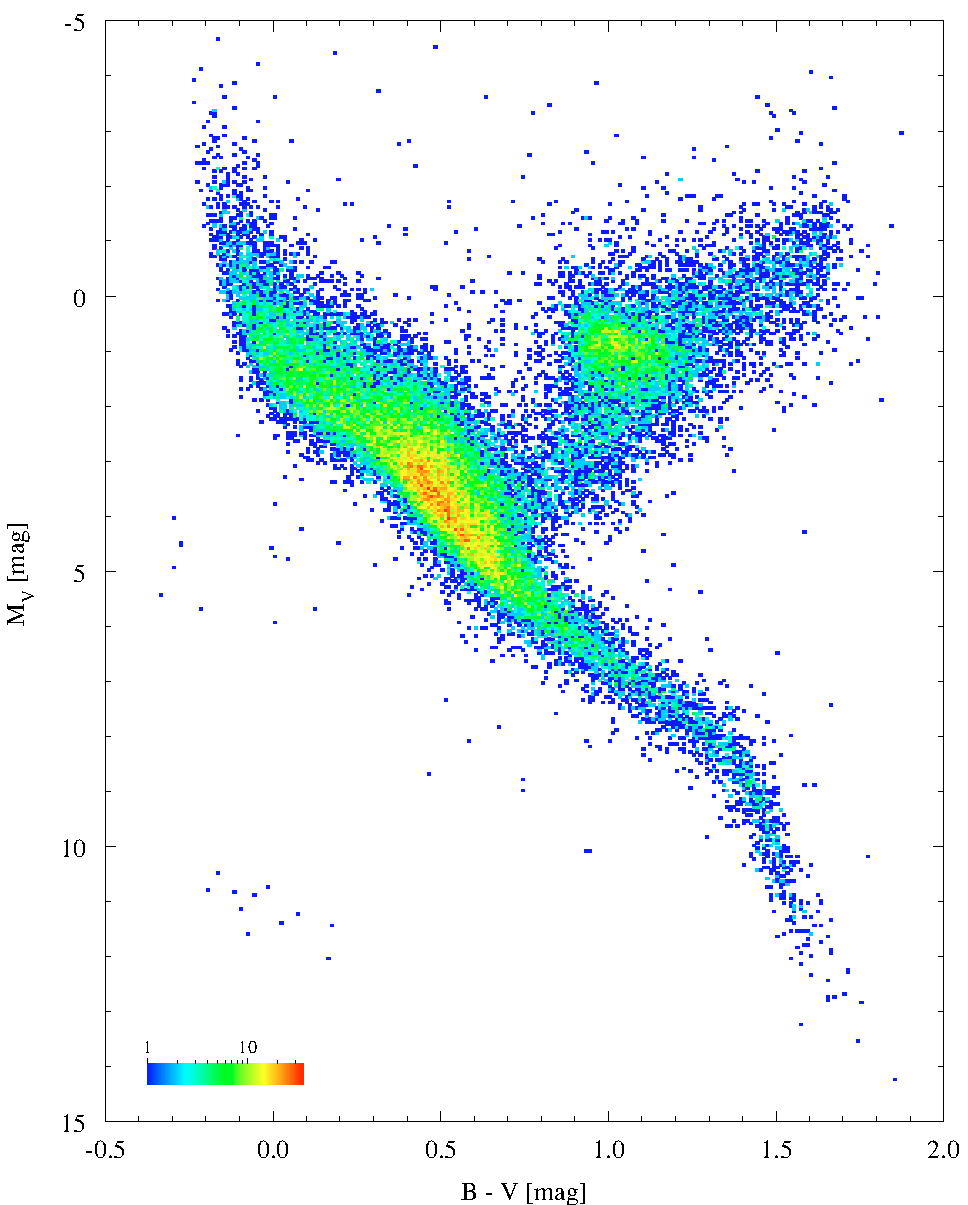
\includegraphics[width=0.75\linewidth]{figures/hr-hip.pdf}
    \caption{Hertzprung-Russel diagram for \(41{,}704\) stars from the Hipparcos Catalogue \citep{Perryman1997}. Colours indicate number of stars in a cell of 0.01 mag in (B-V) and 0.05 mag in V magnitude (\(M_V\)). The main sequence appears as the continuous region extending from the top-left corner of the figure, to the bottom-right corner. The blob above the main sequence, in the top-right region, corresponds to stars in a giant state that have moved out of the main sequence.}
    \label{fig:hr}
\end{figure}

These stars are stable and in a state of \emph{hydrostatic equilibrium}, where gravitational and pressure forces exactly balance each other. The equation of hydrostatic equilibrium is simply the conservation of momentum with zero velocity, \(\fvec{u} = 0\),
\begin{equation}
    \nablavec P = - \rho \nablavec \phi \punct{,}
\end{equation}

which in spherical symmetry can be written as
\begin{equation}
    \frac{\upd P}{\upd r} = - \rho \frac{Gm}{r^2} \punct{,}
\end{equation}

where \(r\) is the distance from the centre of the star and \(m = m(r)\) is the enclosed mass. Together with a description of the composition and nuclear processes taking place in the stellar interior, this gives the complete structure of a star on the main sequence, and is an essential result of the theory of stellar structure.

\subsection{Late stages} \label{sec:star_late}

Every star on the main sequence is supported against gravity by the fusion of hydrogen taking place deep in their core. This process can last from a few million years, to several billion years depending on the mass of the star. The more massive a star is, the faster it will burn its hydrogen. For instance, a star like the Sun is expected to stay on the main sequence for about \(10\) billion years, whereas a star \(50\) times more massive would only last \(\sim3\) million years.

When the core begins to exhaust its available supply of hydrogen, nuclear processes start to slow down. The core thus loses pressure support and contracts under gravity. The star then moves away from the main sequence, and the outcome is once again highly dependent on the total mass of the star.

\subsubsection{Low-mass stars} \label{sec:star_late_lowmass}

Stars of less than about \(8\sunmass\) form a helium core that contracts slowly while the temperature rises in a shell around it. The fusion of hydrogen then moves to this outer shell, leading to an expansion of the star's envelope, but the core stays too cold for helium to burn and continues to collapse on itself. The expansion of the envelope transforms the star into a \emph{red giant}, which can be as large as \(10\text{-}100\sunrad\).

As the core contracts to higher densities, it becomes degenerate, preventing it from collapsing further. This is a consequence of Pauli's exclusion principle, a quantum mechanical effect that forbids fermionic particles, such as electrons, to occupy the same quantum state simultaneously. Because the density has become so high in the core, the electrons are forced to occupy states of higher energy, generating a large pressure. The electron degeneracy pressure can be obtained from the total energy of the free electrons treated as a Fermi gas in the non-relativistic limit (see \citealt{Longair2011} for a complete derivation), and is defined as
\begin{equation}
    P_e = \frac{h^2}{20 m_e} \left( \frac{9}{\pi^2} \rho_e^5 \right)^{1/3} \punct{,}
\end{equation}

where \(h\) is the Planck constant, \(m_e\) the electron mass and \(\rho_e\) the mass density of free electrons in the gas. Electron degeneracy pressure is however independent of the temperature, and stars of \(1\text{-}2\sunmass\) can still reach a temperature high enough for helium burning to take place in the degenerate core with effectively no increase in pressure, while the energy released by the onset of helium fusion further increases the temperature. The consequence is a runaway reaction that fuses most of the helium into carbon over a very short period of time. The large amount of energy released by this reaction can be detected observationally as a \emph{helium flash}.

Stars of higher mass can trigger helium burning before the core reaches degeneracy, therefore producing no helium flash. However, the final outcome stays mostly similar: the contractions of the core will cause the star to \emph{gently} eject its outer layers into a planetary nebula, until only the degenerate core remains. This stellar remnant, known as a \emph{white dwarf}, has a mass of \(0.5\text{-}1.3\sunmass\) and a size comparable to that of the Earth, with a radius of \(\sim6{,}000\units{km}\). It produces no more fusion, and cools down over time.

\subsubsection{Massive stars} \label{sec:star_late_massive}

We henceforth refer to \emph{massive stars} as stars with masses above \(8\text{-}10\sunmass\). These stars burn hydrogen much faster, and the resulting, significantly more massive, helium core collapses much more rapidly than for their lower-mass counterparts. As the pressure and temperature rise quickly, the core reaches helium burning temperatures long before becoming degenerate. This fusion of helium into carbon continues to power the star's core while hydrogen burning moves to a shell around the core that is still hydrogen-rich. Helium depletes much faster than hydrogen, causing the core to collapse once again, until crossing the threshold for carbon and oxygen burning to take place, pushing helium and hydrogen burning further out into the shell. The core undergoes successive phases of fuel exhaustion, during which it further contracts, leading to the burning of heavier and heavier elements while the lighter elements are still burned in a shell structure. This process culminates with the fusion of silicon into iron-group elements, primarily iron and nickel. Since the fusion of these elements is endothermic, the iron produced from the silicon-burning shell does not burn, but rather accretes in an inert core, which quickly becomes degenerate. The final structure of the star is schematised in \Cref{fig:shell_burning}.

Observationally, the star has evolved into either a \emph{red supergiant} or \emph{blue supergiant}. The large amount of energy released by shell burning has caused the outer layers to expand to \(100\text{-}1{,}000\sunrad\), which in turn cools the gas in the envelope. If the star has kept most of its hydrogen envelope, this leads to relatively cold surface temperatures of \(3{,}000\text{-}5{,}000\units{K}\), therefore showing as a red supergiant. However, the envelope becomes more loosely bound to the star, and can easily be ejected by mass-loss processes or gravitational interaction with a binary companion. If the envelope gets ejected, the star evolves into a slightly less large blue supergiant, with surface temperature of \(10{,}000\text{-}50{,}000\units{K}\).

At the final stage of this evolution, the star has completely exhausted its fusion possibilities, and will accumulate iron in its core until it exceeds the Chandrasekhar mass, the limit that can be supported by degenerate electrons. At this point, the iron core typically has a diameter of \(\sim3{,}000\units{km}\) and an average density of \(\sim10^9\units{g/cm^3}\). Nothing can further prevent the core from collapsing, leading to the formation of a neutron star that can either evolve into a black hole if there is enough accretion, in which the entire star eventually falls, or result in a supernova explosion. This is further discussed in \Cref{sec:ccsne}.

\begin{figure}[ht!]
    \centering
    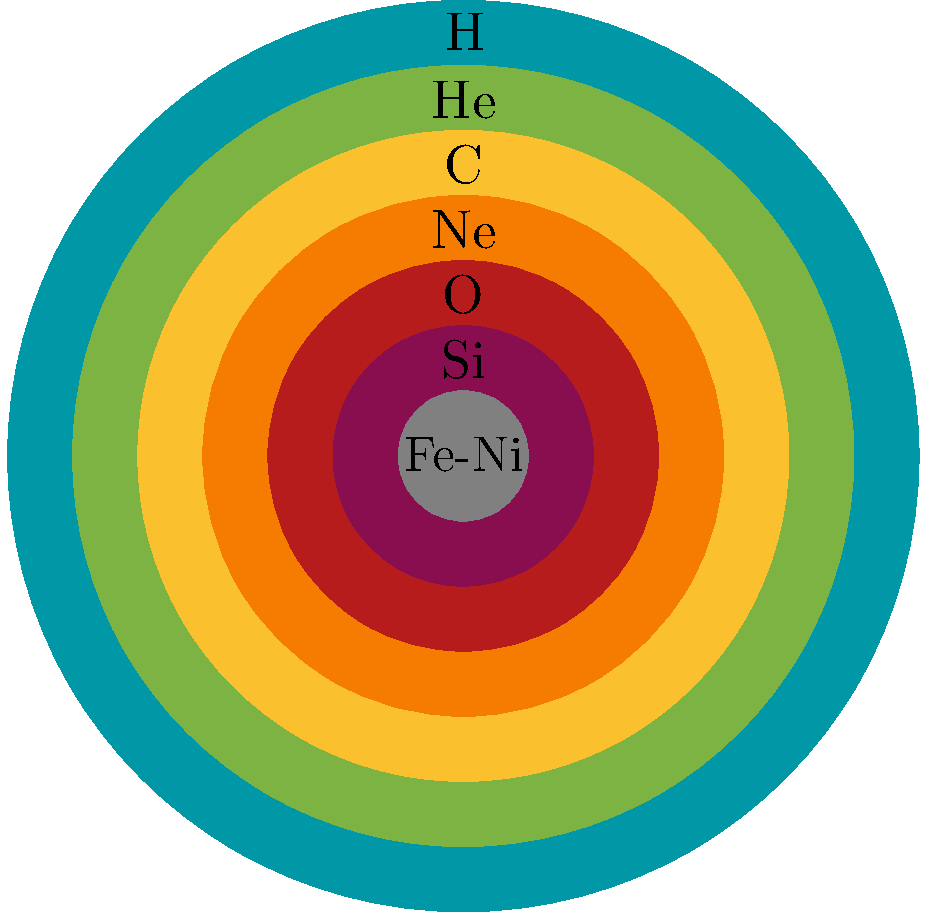
\includegraphics[width=0.5\linewidth]{figures/shell.pdf}
    \caption{Schematic representation of the shell structure of a massive star before the onset of core-collapse. Iron-group elements have accumulated in an inert core at the centre of the star, while lighter elements continue to burn in the outer layers.}
    \label{fig:shell_burning}
\end{figure}

\section{Supernovae} \label{sec:sne}

As we have seen, the late stages of a star's life cycle highly depend on its mass, with the more massive stars exploding as supernovae. We refer to the original object as the \emph{progenitor}. It is the star at the end stage of stellar evolution that leads to the supernova explosion. It can be a single star, or the result of the interaction of multiple stellar bodies. Different progenitors can give rise to very different observable results. In this section, we further define what supernovae are, and discuss both the observational and theoretical properties that characterise them.

\subsection{Observational properties} \label{sec:sne_obs}

Supernovae are transient events, meaning that they can be observed on a human timescale, and can last from a few weeks to several months or even years. They are amongst the most energetic events in the Universe, and can be as bright as an entire galaxy, from millions to billions of times the luminosity of the Sun. Observations of Galactic supernovae, i.e. exploding in our own Milky Way, were already reported by early astronomers of the 11th century and were visible in plain day \citep{Hamacher2014}. This includes, for example, SN 1006 in the Lupus constellation, and SN 1054 whose remnant can still be observed in the Taurus constellation, only \(2\units{kpc}\) away from the Earth, as the well known Crab nebula. The last recorded Galactic supernova was Kepler's supernova in 1604, that exploded about \(6\units{kpc}\) from the Earth, and could be observed with the naked eye. Other unobserved Galactic supernovae were discovered from their remnants, such as Cassiopeia A, estimated to have occurred around 1660-1680 CE \citep{Fesen2006}, \(\sim3.4\units{kpc}\) away from Earth.

It is currently estimated that on average \(\sim1\text{-}3\) supernovae take place per century in a single galaxy \citep{Rozwadowska2021}, therefore the chances of capturing a Galactic supernova are understandably low. Nonetheless, observations of extragalactic events have continuously improved, and automated surveys such as the Zwicky Transient Facility (ZTF) now detect hundreds to thousands of supernovae every year \citep{Fremling2020}.

Supernovae are historically classified according to their observational properties, such as light curves and absorption lines appearing in their spectra. A first classification of supernovae was proposed by \cite{Minkowski1941}, designating supernovae showing hydrogen lines in their spectra as Type II, and those lacking hydrogen lines as Type I. It was then realised that the latter category showed inconsistencies when looking at helium and silicon lines. This category was therefore divided into Type Ia, bearing silicon lines, and Type Ib and Ic, without silicon lines. Type Ib then further shows the presence of helium lines whereas Type Ic does not. \Cref{fig:sn_curves} shows example spectra corresponding to these different classifications. Type II was also further extended into, notably but not exclusively, Type II-P and Type II-L depending on properties of the light curve. After reaching a peak in luminosity, Type II-P supernovae experience a period of nearly constant brightness, a plateau, that can last for about 100 days. On the contrary, Type II-L supernovae show a continuous, almost linear decline of their brightness over time. See \cite{Cappellaro2001} for a more detailed discussion on the supernova classification scheme.

\begin{figure}[ht!]
    \centering
    %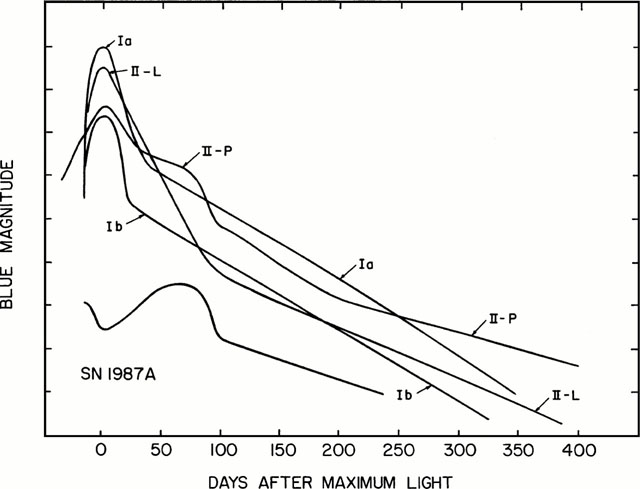
\includegraphics[width=0.75\textwidth]{figures/sn_curves1.jpg}
    %\caption{Typical light curves for different types of supernovae, along with the light curve of SN 1987A. Figure taken from \cite{Filippenko1997}.}
    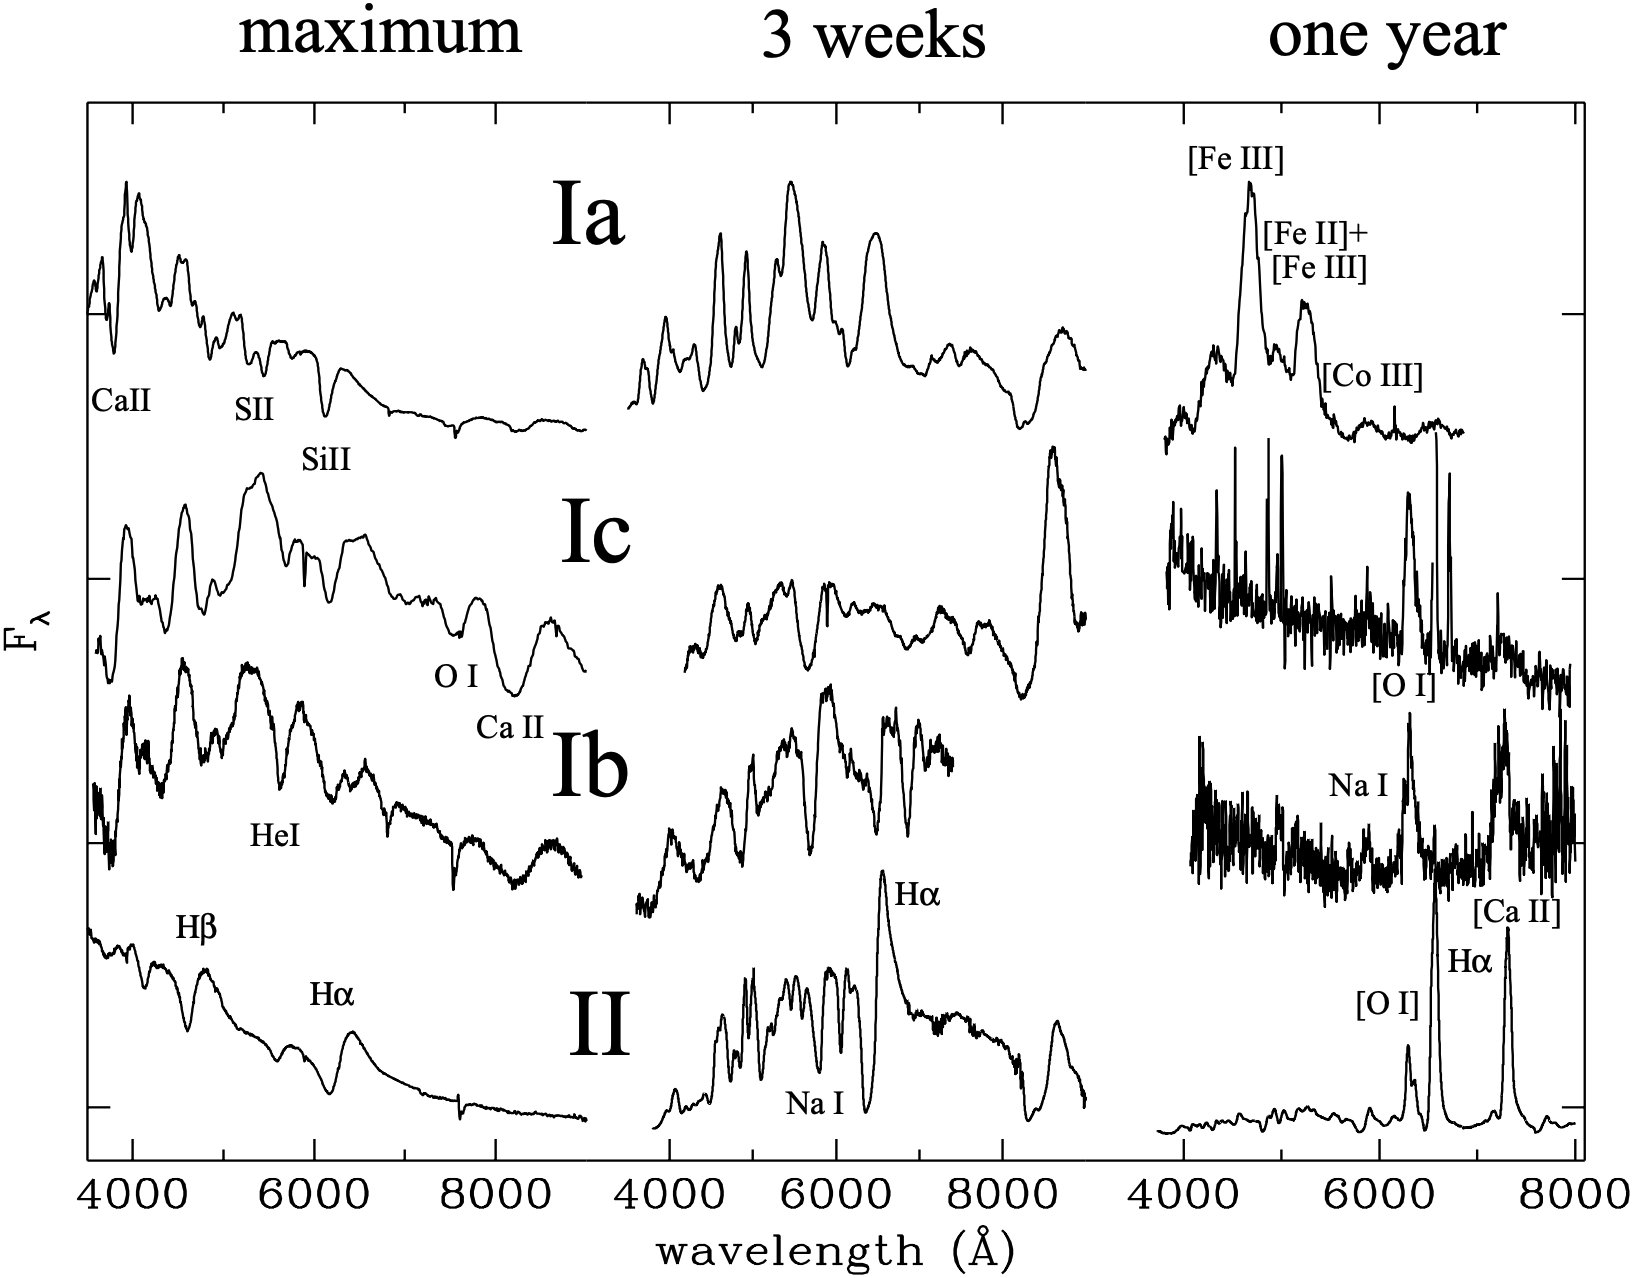
\includegraphics[width=0.75\textwidth]{figures/sn_curves.png}
    \caption{Representative spectra for Type Ia, Ib, Ic and II supernovae, at peak luminosity (left), 3 weeks after (middle) and 10 months after (right). Figure taken from \cite{Turatto2003}.}
    %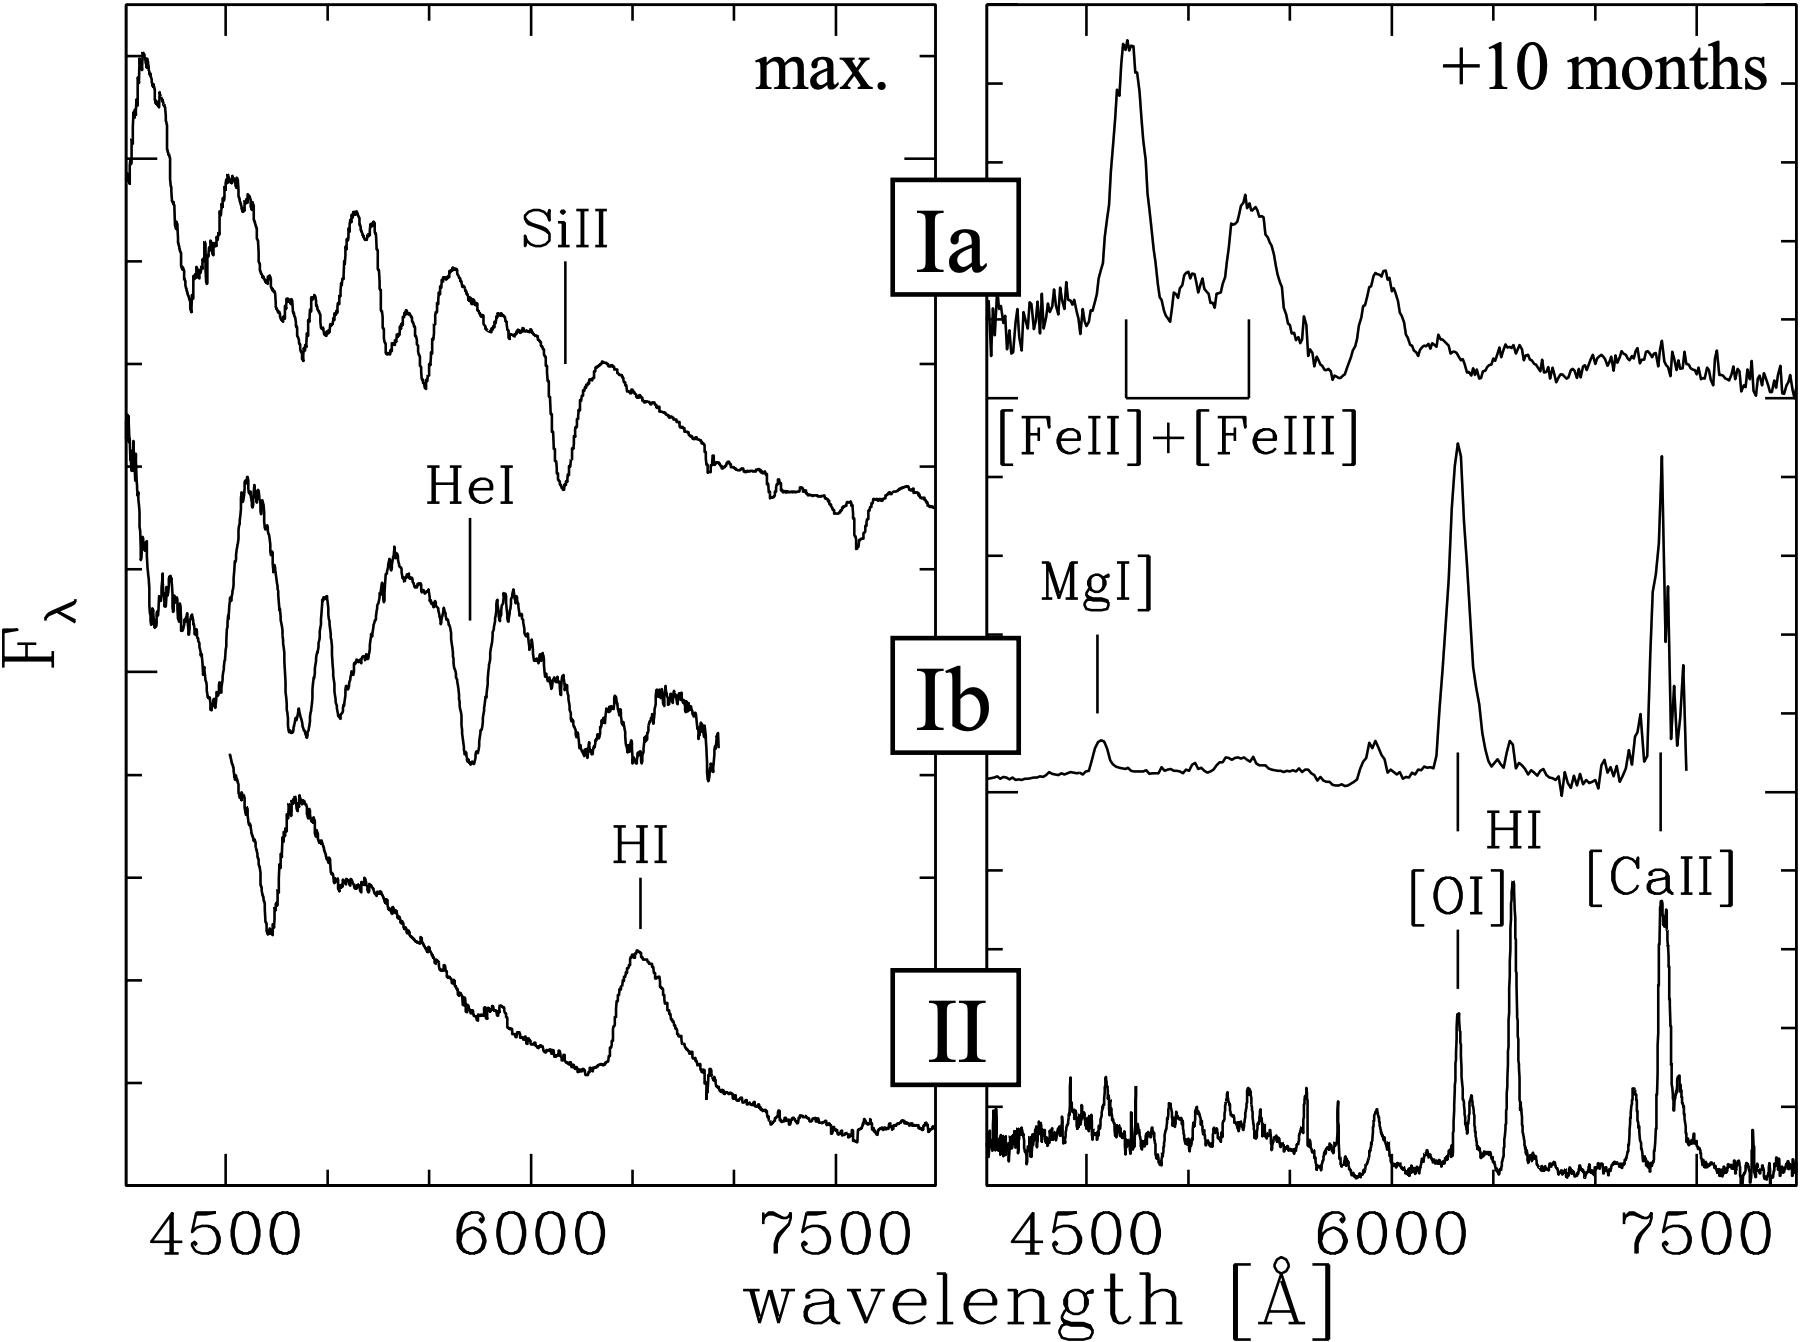
\includegraphics[width=0.75\textwidth]{figures/sn_curves2.png}
    %\caption{Representative spectra for Type Ia, Ib and II supernovae, at peak luminosity (left panel) and at 10 months after (right panel). Figure taken from \cite{Cappellaro2001}.}
    \label{fig:sn_curves}
\end{figure}

\subsection{Explosion mechanism} \label{sec:sne_exp}

From a theoretical point of view, we adopt another approach at classifying supernovae based on the explosion mechanism. The observational classification of supernovae is easily subject to factors such as stellar winds, interactions with the circumstellar medium or evolution in multiple systems, explaining the large amount of subcategories due to altered observable properties. Conversely, a classification based on the explosion mechanism leads to mainly two, well defined, categories: \emph{thermonuclear} and \emph{core-collapse supernovae}. We should note however that the term \emph{core collapse} usually refers more specifically to \emph{iron-core collapse}, and that we focus on this particular type in this thesis. However, a category of \emph{oxygen-core-collapse supernovae}, known as \emph{Electron-Capture Supernovae} (ECSNe), exists and is briefly discussed as well in this section.

\subsubsection{Thermonuclear} \label{sec:sne_exp_ia}

We have discussed electron degeneracy pressure and noted that it is temperature independent. A degenerate star, such as a white dwarf, that were to exceed the Chandrasekhar limit of about \(1.44\sunmass\) would lose pressure support from degenerate electrons and collapse. The collapse would lead to an increase in temperature that would not be balanced by an increase in pressure, thereby reigniting the star. The nuclear reaction rates would then enter a feedback loop and accelerate exponentially, ultimately disrupting the entire star.

White dwarfs composed of carbon and oxygen, the remnants of low-mass stars, are believed to be the progenitors of Type Ia supernovae, and explode due to the ignition of carbon \citep{Mazzali2007}. It is thought however that the star can ignite before the Chandrasekhar limit is attained, and therefore never actually collapses. Type Ia supernovae are the most commonly detected supernovae, partly due to their very high brightness that allows them to be detected from much farther away. Although it is not clear what causes a white dwarf to accumulate excessive mass, and there is no consensus on the matter, it is usually thought to be the result of accretion from a companion star, typically a red giant or supergiant with a loosely bound envelope, or the coalescence of two white dwarfs.
%\haakon{they can just never agree on which one it is}
These progenitors have the particularity of not leaving any remnant, as the entire star is destroyed.

Another type of thermonuclear supernova is the Pair-Instability Supernova (PISN). Very massive stars (\(\gtrsim 140\sunmass\)) have interiors significantly supported against gravity by photon pressure. Due to the very high temperatures, these photons are mostly in the form of gamma rays, which have the property of interacting with each other to form an electron--positron pair. If the temperature and gamma ray density become high enough, the increasing production of electron--positron pairs will cause a loss of support from radiation pressure and render the star unstable to collapse. This further increases the temperature and accelerates the production of gamma rays, until the ignition of oxygen in a runaway process results in the disruption of the entire star in an extremely energetic supernova, leaving no remnant (see section VII in \citealt{Woosley2002} for a detailed description).

The explosion mechanism of PISNe is perhaps the most well understood theoretical model of supernovae. Paradoxically, no PISN has ever been observed despite being predicted to be \(\sim100\) times brighter than Type Ia supernovae. However, theoretical models of nucleosynthetic yields from PISNe have allowed to confirm their existence from the observation of very metal-poor stars in the Milky Way halo, that would have formed from the ejecta of a PISN in the early Universe \citep{Xing2023}. Some PISN candidates have been reported (\citealt{Schulze2024, GalYam2009} for example) but have never been unambiguously classified as such.
%\haakon{I think come candidates exists, but I am not sure. Maybe one of the observers know, could be cool to throw in a reference to a candidate. The PPI supernovae are also interesting for black hole masses.}

\subsubsection{Core collapse} \label{sec:ccsne}

In \Cref{sec:star_late_massive}, we have discussed the mechanisms that lead to the formation of an inert iron core in massive stars. The degenerate core eventually collapses into a neutron star, an extremely compact object of only \(\sim30\units{km}\) in diameter and with a density comparable to several times that of atomic nuclei of about \(10^{14}\units{g/cm^3}\).

The contraction of the iron core results in two important processes, both of which accelerates the collapse. The first is the increasing rate of photodisintegration of iron-group elements. The high temperature breaks the atomic nuclei into free nucleons and alpha particles, which consumes a large amount of thermal energy, therefore decreasing the pressure. The second is a consequence of the rise in density, that accelerates the rate at which free electrons are captured by protons and nuclei, following the reactions
\begin{gather}
    e^{-} + p \rightarrow n + \nu_e \punct{,} \label{eq:nu_e} \\
    e^{-} + (\mathcal{A}, \mathcal{Z}) \rightarrow (\mathcal{A}, \mathcal{Z} - 1) + \nu_e \punct{,} \label{eq:anu_e}
\end{gather}

where \(p\), \(e^{-}\), \((\mathcal{A}, \mathcal{Z})\) and \(\nu_e\) represents a proton, an electron, a nucleus of atomic mass \(\mathcal{A}\) and atomic number \(\mathcal{Z}\), and an electron neutrino, respectively. The pressure support from degenerate electrons is progressively lost as the core becomes more neutron-rich. The neutrinos produced from the above reactions carry energy away and \emph{deleptonise} the core, effectively reducing the Chandrasekhar mass.

% At higher temperature/density, a population of positrons lead to
%   n + e^{+} \rightarrow p + \bar{\nu_e}
% Also pair processes
%   e^{+} + e^{-} \rightarrow \nu_e + \bar{\nu_e}
% and much more (Urca processes when NS cools)

% There's so much to say omg

When the core reaches nuclear densities, due to the repulsive forces between nucleons, the equation of state of matter stiffens, producing a pressure strong enough to abruptly halt the collapse. However, the high inertia of the collapsing core has caused it to contract beyond the equilibrium point and, as a result, the pressure rapidly pushes the core outwards to restore balance with gravity. The inner region of the iron core then collides with the infalling material from the outer shell, resulting in the formation of a shock wave. This moment is referred to as the \emph{core bounce}.

The shock wave propagates outwards through the supersonically infalling shells of material above. The ram pressure on the shock front and the disintegration of the heavy nuclei into free nucleons causes the shock to quickly lose a significant amount of energy. After only \(\sim100\units{ms}\), the shock begins to stall at about \(100\units{km}\) above the proto-neutron star (PNS).

In order for the shock to be revived and the star to explode in a supernova, additional energy must be deposited in the shock front. We remember that the gravitational potential energy can be expressed as
\begin{equation}
    \mathcal{W} \sim \frac{GM^2}{R} \punct{.}
\end{equation}

Calculating this quantity for a PNS (\(M \sim 1.5\sunmass\) and \(R \sim 30\units{km}\)), we see that the collapse of the iron core releases \(\Delta \mathcal{W} \sim 10^{53}\units{erg}\). This energy is initially transformed into thermal energy resulting in the formation of a hot PNS with initial temperature of a few \(10^{11}\units{K}\). Under such conditions of temperature and density, neutrinos dominate the cooling inside the PNS, until most of the binding energy is converted to neutrinos. Neutrinos are weakly interacting particles, and baryonic matter is mostly transparent to them. However, the density in the PNS is high enough to trap the neutrinos, and it takes time, of the order of seconds, for the neutrinos to diffuse out of the PNS. Once the neutrinos escape the neutrinosphere, the high densities at the shock front then allows a portion of the neutrinos to interact, injecting \(\sim1\%\) of the total neutrino energy released, or about \(10^{51}\units{erg}\), directly behind the shock, in a region called the \emph{gain region}. Although only a small amount of neutrinos interact, this is enough to revive the shock, which will continue to propagate through the envelope and explode the star. This mechanism was proposed by \cite{ColgateWhite1966} and later revisited by \cite{Wilson1985}, now known as the \emph{delayed neutrino-driven explosion mechanism} \citep{Bethe1985}. The shock reaches the surface of the star on a timescale of several hours to a few days, and the photons that were trapped behind escape, becoming visible as either a Type Ib/c or Type II supernova.

It is worth noting that, if neutrinos are assumed to be the driving mechanism behind shock revival, this is largely aided by turbulence and instabilities, such as convection, arising in the gain region due to the neutrino heating \citep{Burrows1995}. For this reason, one-dimensional simulations of CCSNe, that fail to account for these multidimensional effects, do not result in successful explosions for most progenitors, except for some of the lowest mass ones \citep{Kitaura2006}. The determination of the exact processes involved and the consequences of these instabilities is still an active area of research.

\subsubsection{Electron capture} \label{sec:ecsne}

In the mass range of \(8\text{-}10\sunmass\) that separates low-mass stars, that turn into white dwarfs, and massive stars, that collapse into neutron stars and black holes, there exist a transitional category of supernovae known as electron-capture supernovae. \cite{Miyaji1980} initially proposed that stars in this mass range could reach temperatures high enough to initiate carbon burning in their core, but not enough to fuse heavier elements, leading to the formation of a degenerate core composed of oxygen, neon and magnesium (ONeMg core). The collapse of the ONeMg core would then be triggered after reaching densities high enough that electron capture processes on neon and magnesium nuclei become significant. In much the same way that was discussed in the previous section on core collapse, electron capture emits neutrinos, deleptonising the core and reducing its effective Chandrasekhar mass, until the collapse of the core into a neutron star becomes inevitable. Observational evidence of ECSNe was found only recently, and it was suggested that the Crab nebula was most likely due to an ECSN \citep{Hiramatsu2021}.

\section{Simulations} \label{sec:sims}

The inherent inability of conventional telescopes to observe the processes taking place deep in the core of dying stars, and the impossibility to reproduce such extreme conditions of density and temperature in laboratories makes the study of supernova explosions a mostly theoretical field.  By developing theoretical and numerical models of supernovae, it becomes possible to guide observations for clues of certain processes, which in turn provides constraints on the otherwise large theoretical parameter space. As an example, we have mentioned the neutrino-driven explosion mechanism for CCSNe proposed by \cite{ColgateWhite1966} that was later supported by the direct detection of neutrinos from the SN 1987A event that occurred in the Large Magellanic Cloud \citep{Hirata1987, Bionta1987, Burrows1987}. In the same way, numerical models of nucleosynthetic yields from PISNe progenitors have been found to match the abundance patterns of very metal-poor stars in the Galactic halo \citep{Xing2023}.

Researchers have been developing numerical models and performing simulations of CCSNe since the late 1960s. The exponential increase in the available computational power has allowed the inclusion of more and more detailed physics over time, starting from simple, one-dimensional, hydrodynamical models powered by pistons, to multidimensional and multiphysics simulations (see \citealt{Janka2012, Mezzacappa2020, Boccioli2024} for detailed reviews and references). However, the complexity of such simulations present a number of challenges and can lead to extreme computational costs, therefore, approximations must be made. For example, a full Boltzmann transport of neutrinos is prohibitively expensive in most situations, and a majority of state-of-the-art simulation codes rather implement approximations based on, for example, moment schemes, leakage or Monte Carlo algorithms (see \citealt{Foucart2023,Mezzacappa2020_Review} for a detailed description of these algorithms). In a similar way, it was shown that a Newtonian approximation of gravity was not acceptable to simulate the central engine of CCSNe \citep{Muller2012,OConnor2018a}, but approximate general relativistic solutions can be used in order to avoid a complete general relativistic treatment. However, the impact of different assumptions and algorithms on the accuracy of the resulting simulations must be carefully tested and analysed, and informed choices on the parameter space to explore must be made.

The description of supernovae involves physics from many different fields, such as magneto-hydrodynamics (MHD), neutrino interactions and nuclear physics, most of which are active areas of research, each carrying a wide range of uncertainties. As a result, self-consistent simulations of CCSNe are hard to achieve, and results from various groups, using different codes, most often do not agree with each other. Furthermore, the computational cost heavily limits the timescales that can be simulated. Most simulations only focus on the first few hundred milliseconds to seconds after core bounce. Long-term simulations, that can evolve from minutes to hours after bounce and reach shock breakout, are very rare, but are nonetheless essential to link simulations to observations. Moreover, such simulations are of particular interest for studying explosive nucleosynthesis and the final composition of the supernova ejecta. This research is crucial to better understand subjects such as galactic chemical evolution and the origin of heavy elements beyond the iron peak, particularly \emph{r}-process elements (see \citealt{Arcones2023} for a review). 
In this work, we have explored the achievability of long-term simulations of CCSNe at a reasonable computational cost based on the formation of a neutrino-driven wind around the PNS in the first seconds after bounce. We do so by excising the central region of the star, where the PNS is located, and replacing it with an inner boundary condition that mimics this neutrino wind. This method is presented in \Cref{chap:methods}.

\section{Neutrino-driven winds} \label{sec:ndw}

At the moment of collapse, the gravitational binding energy released by the formation of the PNS is transformed into thermal energy. The high temperatures inside the PNS trigger nuclear processes that convert most of this energy into neutrinos. However, these neutrinos are originally trapped inside the PNS due to the high densities, and slowly diffuse through the inner core before escaping the neutrinosphere, carrying away energy and cooling the neutron star. The neutrinosphere is the region outside the PNS that presents steep gradients in density and temperature, and where the mean free path of the neutrinos become comparable to the size of the PNS. A fraction of the escaping neutrinos interact with matter in this region, following the inverse reactions of \Cref{eq:nu_e,eq:anu_e}, depositing energy that blows off matter from the surface of the neutron star. If no matter is being accreted on the PNS, this outflow can become supersonic and form a \emph{neutrino-driven wind}. This neutrino-driven wind is usually characterised by a relatively smooth, quasi-spherically symmetric profile, forming \(\sim1\units{s}\) after bounce. At this point, the shock has been successfully launched and has propagated to sufficiently large radii (\(\sim10{,}000\units{km}\)) that it has little to no effects on the conditions in the region of interest. The PNS, however, continues to cool on the Kelvin-Helmholtz timescale for a few tens of seconds after the explosion. During this period, the neutrino luminosities and the properties of the neutron star (mass, radius and temperature) change very slowly. This description was supported by simulations by \cite{Janka1995}, and allows us to express the hydrodynamics of the outflow using a quasi-steady state approximation, so that mass, momentum and energy conservation can be written in spherical symmetry as
\begin{gather}
    \dot{M} = 4 \pi r^2 \rho u \punct{,} \\
    u \frac{\upd u}{\upd r} = - \frac{1}{\rho} \frac{\upd P}{\upd r} - \frac{GM}{r^2} \punct{,} \\
    \dot{q} = u \left( \frac{\upd \mathcal{E}}{\upd r} - \frac{P}{\rho^2} \frac{\upd \rho}{\upd r} \right) \punct{,}
\end{gather}

where \(\rho\), \(P\), \(u\) and \(\mathcal{E}\) denote the density, pressure, flow velocity and specific internal energy, respectively, and \(M\) is the mass of the neutron star, \(\dot{M}\) is a constant mass outflow rate, and \(\dot{q}\) is the specific heating rate due to neutrino interactions. Note however that the pressure and specific internal energy accounts for non-relativistic nucleons as well as relativistic particles (electrons and positrons) and photon radiation. This description of the neutrino-driven outflow from the hot neutron star was first brought forth by \cite{Duncan1986}.

In reality, the conditions in the wind may be more complex, and influenced by late accretion on the PNS, rotation, or continued convection in the gain region. It is however a convenient approximation to explore the impact of the neutrino wind on the nucleosynthesis and dynamics of the inner-most ejecta of the supernova, near the PNS. In particular, the implications of the neutrino-driven wind as a potential site of production of heavy elements by rapid neutron capture, known as \emph{r}-process, have been under investigation since the early 1990s. Under the steady state assumption, \cite{Qian1996} identified the key parameters characterising the neutrino wind that describe the nucleosynthesis in the ejecta: the mass loss rate, the entropy per baryon, the expansion timescale and the electron fraction. The latter parameter, the electron fraction, is defined as
\begin{equation}
    Y_e = \sum_i \left( \frac{Z_i}{A_i} \right) X_i \punct{,}
\end{equation}

where \(Z_i\), \(A_i\) and \(X_i\) are the atomic charge, mass number and mass fraction of species \(i\), respectively. It is used to define whether the ejecta is neutron-rich (\(Y_e < 0.5\)) or proton-rich (\(Y_e > 0.5\)), and is importantly influenced by neutrinos, where the competing interactions of electron neutrino and antineutrino capture usually renders the wind more proton-rich in the context of neutrino-driven supernovae. As a consequence, a strong \emph{r}-process in the neutrino wind does not seem possible in neutrino-driven supernovae. However, a weak \emph{r}-process is possible and can contribute to the formation of the lighter heavy elements, from strontium to silver \citep{Arcones2014}. In the case of more proton-rich conditions, another process known as the \(\nu p\)-process can take place \citep{Frohlich2006,Nevins2024}. Furthermore, exotic supernovae such as magneto-rotational supernovae and collapsars, are thought to be potential sites of strong \emph{r}-process. Although the subjects of nucleosynthesis and explosive burning in CCSNe are not further developed for the purpose of this thesis, they are nonetheless essential aspects of this field, and we refer the interested reader to \cite{Arcones2013, Boccioli2024} for reviews.


\mainchapter{Methods}{0.55}{After some tedious algebra, that is left as an exercise to the reader\ldots}{E. Landi Degl’Innocenti,\\\textit{Polarization in Spectral Lines}} \label{chap:methods}

%----------------------------------------%
% Methods
%----------------------------------------%

We have performed long-term simulations of CCSNe in one and two dimensions, from \(\sim1\units{s}\) after bounce until shock breakout from the stellar surface, several tens of hours afterwards. To do so at a reasonable computational cost, we have implemented an inner boundary condition designed to mimic the neutrino-driven wind forming around the PNS. This chapter presents the progenitors and the tools used for the simulations as well as the details of the methods employed.

\section{Numerical setup} \label{sec:setup}

In this thesis, we used two progenitors to perform 1D and 2D simulations. The 1D simulations utilised a zero-metallicity, \(M_\mathrm{ZAMS} = 9.6\sunmass\) progenitor star from A. Heger (private communication), and the 2D simulations utilised a solar-metallicity, \(M_\mathrm{ZAMS} = 12\sunmass\) progenitor from \cite{Woosley2007} (thenceforth referred to as the z9.6 and s12 progenitors, respectively). Note that we refer to the Zero-Age Main-Sequence (ZAMS) mass, which corresponds to the mass of the star at its entry on the main sequence. The final mass of the star at moment of collapse is determined by processes such as stellar winds, that have caused it to lose mass during the course of its life, and depends on the stellar evolution models used to produce the progenitor.

The simulations are carried out in two phases. A first simulation is ran from moment of collapse until \(\sim1\text{-}2\units{s}\) after core bounce, and a second, long-term simulation continues until shock breakout from the stellar surface using the inner boundary conditions described in \Cref{sec:bdry_condition} along with simpler physics. 

\subsection{FLASH}

All the simulations presented in this thesis are carried out utilising a modified version of the \flash\ framework (version 4) \citep{Fryxell2000, Dubey2009}. The \flash\ code is a modular, multiphysics, Newtonian hydrodynamics code. It can simulate using spherical coordinates in one dimension, assuming spherical symmetry, with cylindrical coordinates in two dimensions, assuming axisymmetry, and with Cartesian coordinates in three dimensions, assuming no symmetry. \flash\ uses a uniform grid with Adaptive Mesh Refinement (AMR). AMR is a numerical technique used to refine the grid locally in order to obtain a higher resolution where needed, whilst saving computational time in places where a lower resolution is sufficient. Refinement and derefinement is determined by a user-defined error criterion, and the time step is set by the Courant–Friedrichs–Lewy (CFL) condition. In \flash, this condition is written as follows
\begin{equation}
    C = (c_s \pm u) \frac{\Delta t}{\Delta x} \punct{,}
\end{equation}

where \(c_s\) and \(u\) are the local sound speed and flow velocity, \(\Delta t\) is the local time step and \(\Delta x\) is the cell size. The value of the CFL condition \(C\) being known from the configuration of the simulation, \flash\ can solve for the time step using the largest value of \(c_s \pm u\). In \flash, the domain is subdivided in regions called \emph{blocks} that can achieve different levels of refinement. Each additional level of refinement cuts the size of a block in half in each direction, and the block at the highest refinement level is divided in 16 grid cells in every direction. Additionally, \flash\ restricts the jump in refinement from one block to an adjacent one to no more than one level. An example block structure is pictured in \Cref{fig:flash_blocks}.

\begin{figure}[ht!]
    \centering
    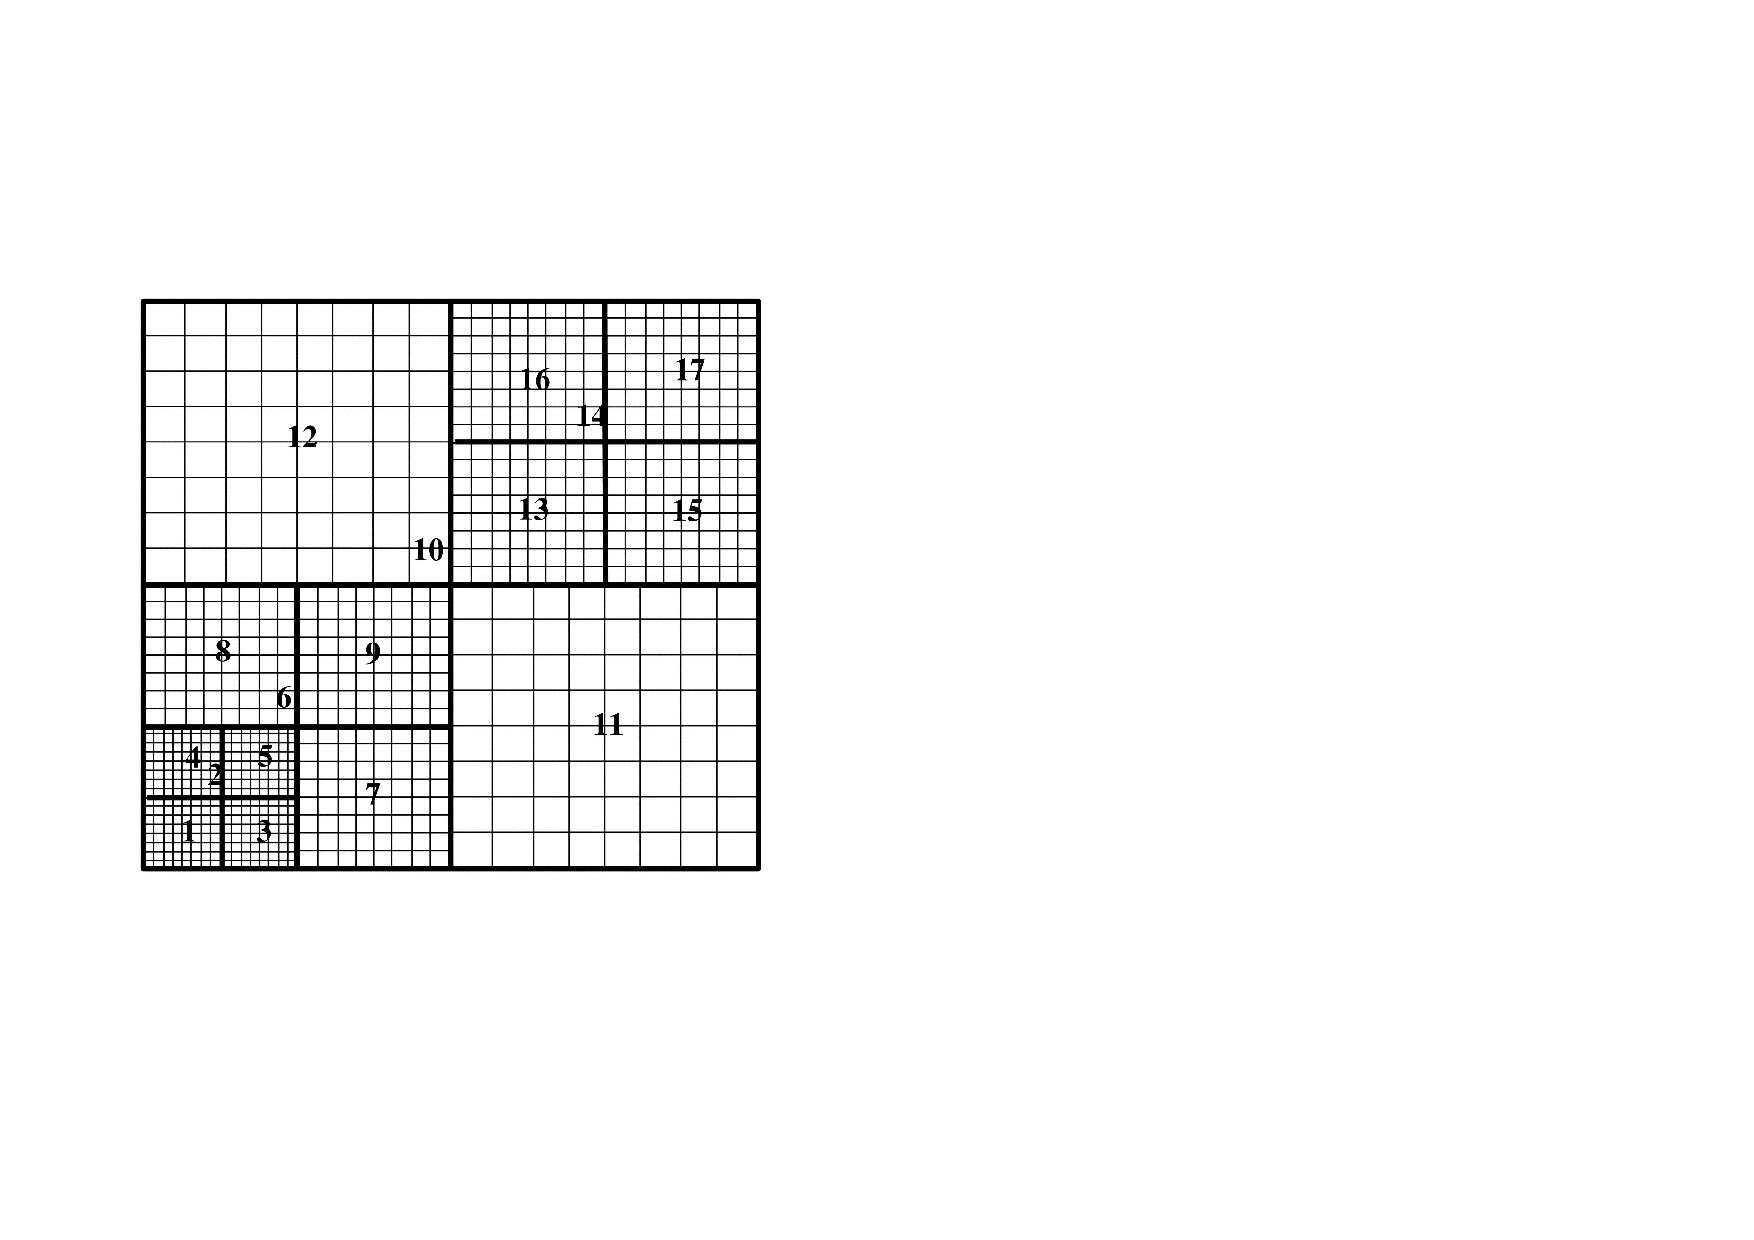
\includegraphics[width=0.55\linewidth]{figures/flash_blocks.pdf}
    \caption{An example set of blocks in \flash. In this example, an interior grid structure of 8x8 cells is also shown, but we use 16x16 for our simulations. The numbers near the centre of the blocks show where the blocks are located in the list of blocks, not shown here. Figure taken from \cite{Fryxell2000}.}
    \label{fig:flash_blocks}
\end{figure}

We use a version of \flash\ specifically adapted for core collapse simulations \citep{Couch2013, Couch2014, OConnor2018a, OConnor2018b}. The code uses a modified general relativistic effective potential to solve gravity (Case A in \citealt{Marek2006}), and evolves three neutrino species using an energy-dependent two-moment neutrino transport scheme with an analytical closure (M1) \citep{OConnor2018a}. This includes electron neutrinos and antineutrinos, as well as a third species collecting all the heavy-lepton neutrinos. Neutrino opacities are generated with the neutrino opacity library NuLib \citep{OConnor2015, Sullivan2016}.

\subsection{Collapse and post-bounce setup} \label{sec:cc_setup}

The z9.6 progenitor is simulated from collapse until \(2.23\units{s}\) after collapse in spherical symmetry (1D) on a domain extending to a radius of \(10^{11}\units{cm}\). Using 16 levels of adaptive mesh refinement, we achieve a finest grid spacing of \(\sim238\units{m}\), with the largest cells being \(\sim7{,}800\units{km}\) across. The energy-dependent neutrino transport is carried out using 12 energy groups. The simulation uses a hybrid EoS, made from a combination of two equations of state. At nuclear densities, such as in the PNS, the SFHo equation of state is used \citep{Steiner2013}, then at lower densities, outside of the PNS, the so-called \emph{Helmholtz EoS} is used instead \citep{Timmes1999}. The latter EoS gives the pressure from the contribution of different species,
\begin{equation}
    P = P_\mathrm{rad} + P_\mathrm{ion} + P_\mathrm{ele} + P_\mathrm{pos}
\end{equation}

where \(P_\mathrm{rad}\), \(P_\mathrm{ion}\),  \(P_\mathrm{ele}\) and  \(P_\mathrm{pos}\) is the radiation pressure, the pressure from the nuclei, and the electron and positron pressures respectively. The different contributions can be computed analytically from the temperature \(T\), the density \(\rho\), the mean number of nucleons per isotope \(\bar{\mathcal{A}}\) and the mean charge per isotope \(\bar{\mathcal{Z}}\), following \cite{Timmes1999}.

The s12 progenitor is simulated from collapse until \(\sim1.2\units{s}\) after collapse in cylindrical coordinates using axisymmetry on the polar axis (2D). The domain extends to a radius of \(6.4 \cdot 10^9\units{cm}\) and covers \(\pm 6.4 \cdot 10^9\units{cm}\) along the polar axis. The simulation uses 11 levels of refinement to obtain a minimum grid spacing of \(\sim488 \units{m}\) in the PNS and maintains an angular resolution of \(0.6\degree\). The simulation uses the same parametrisation for the neutrino transport as for the z9.6 as well as the same EoS. This progenitor has been simulated three times with different heating factors \(f_\mathrm{heat}\) of \(1.0\), \(1.5\) and \(2.0\), i.e a heating factor of \(2.0\) will result in twice as much energy deposited by neutrinos in the gain layer as it should normally do. 
This was done in order to obtain different explosion energies and observe the impact on the explosion mechanism and the evolution of the shock wave.
For simplicity, we henceforth refer to this set of simulations, before time of mapping, as the \emph{initial simulations}.

\subsection{Long-term setup} \label{sec:lt_setup}

To save computational time, the initial simulations are performed only on the most central part of the progenitors for a sufficiently short duration that the shock wave stays far from the boundaries of the domain and that the outer envelope can be assumed to be in equilibrium. Thus, in order to continue the simulation until shock breakout, we must first map the final state of the first simulation, at time of mapping \(t_\mathrm{map}\), to a larger domain that contains the entire star. Because the progenitor models are given in the form of 1D profiles, extending the domain for the 1D simulation is straightforward. The mapping procedure is a little more complex in 2D, but is in essence very similar: we map the result of the initial simulation at time of mapping onto the original progenitor model in order to include the outer parts of the progenitor to the computational domain. More details on the mapping procedure are given in \Cref{sec:mapping}

The long-term simulations are carried out in two steps. First using the outflow boundary condition, described in \Cref{sec:bdry_out}, until the diagnostic explosion energy saturates, which corresponds to approximately the Kelvin-Helmholtz cooling timescale of \(\sim 10\units{s}\). Afterwards, we use the inflow boundary condition, described in \Cref{sec:bdry_in}, for the rest of the simulation until shock breakout. Consequently, the neutrino transport is turned off for these simulations, and the need for a high-density equation of state is eliminated, as the PNS is cut from the domain and replaced by the inner boundary condition. Therefore, only the Helmholtz EoS is used, and a lower resolution of the computational grid is sufficient.  To prevent ambiguities, it should be noted that it is common to refer to the terms \emph{inflow} and \emph{outflow} in the sense of matter flowing in or out of the domain. In this thesis, however, we will refer to \emph{inflow} and \emph{outflow} in the opposite way, as matter flowing towards or away from the PNS.

The long-term simulation of the z9.6 progenitor is ran from \(t_\mathrm{map} = 1.6\units{s}\) after collapse until shock breakout. The new domain extends to \(1.49 \cdot 10^{13}\units{cm}\) and uses 18 levels of refinement, giving a minimum grid spacing of \(\sim8.9\units{km}\).

The long-term 2D simulations of the s12 progenitor are ran from \(t_\mathrm{map} = 1.15\units{s}\) after collapse until shock breakout, the new domain extending to a radius of \(5.24 \cdot 10^{13}\units{cm}\) and covering \(\pm 5.24 \cdot 10^{13}\units{cm}\) along the polar axis. It uses 20 levels of refinement and maintains an angular resolution of \(0.6\degree\), giving a minimum grid spacing of \(\sim7.8\units{km}\).

For all the simulations, the outflow boundary condition is fixed at a radius of \(500\units{km}\). The conditions at the inner boundary are taken from the initial simulations at time of mapping. For the 1D simulation, this is simply the values of the density, internal energy and velocity at \(500\units{km}\). The conditions for the 2D simulations are obtained by spherically averaging the relevant quantities. Unfortunately, for most of the simulations, this gives rather unrealistic values of the velocity, either very low, extremely high, or negative. Thus, most of the 2D simulations were ran with different wind velocities, and the influence of this choice is explored in \Cref{chap:results}. An overview of the long-term simulations and their parametrisation is shown in \Cref{tab:sim_params}, where the different simulations have been labelled based on a combination of the progenitor name, and optionally the heating factor and neutrino wind velocity, in this order.

\begin{table}[ht!]
\begin{threeparttable}[t]
    \caption{Overview of the long-term simulations.}
    \label{tab:sim_params}
    \centering
    \setstretch{1.2}
    \begin{tabular*}{\columnwidth}{@{\extracolsep{\stretch{1}}}*{8}{c}@{}}
    \hline
    \hline
    Name            & Progenitor & \(f_\mathrm{heat}\) & \(t_\mathrm{map}\)\tnote{a} & \(t_\mathrm{hole}\)\tnote{b} & \(v_\mathrm{wind}\) & \(\gamma_{\rho}\) & \(\gamma_{e}\) \\ 
                    &            &                     & [s]                         & [s]                          & [km/s]              &                   &                \\ \hline
    z96             & z9.6       & 1.0                 & 1.6                         & 30.0                         & \(11{,}357\)          & 1.8               & 0.06           \\
    s12hf1p0\_w10e8 & s12        & 1.0                 & 1.15                        & 8.0                          & \(10{,}000\)          & 1.8               & 0.6            \\
    s12hf1p0\_w28e8 & s12        & 1.0                 & 1.15                        & 8.0                          & \(28{,}000\)          & 1.8               & 0.6            \\
    s12hf1p5\_w13e8 & s12        & 1.5                 & 1.15                        & 10.0                         & \(13{,}000\)          & 1.8               & 0.6            \\
    s12hf1p5\_w15e8 & s12        & 1.5                 & 1.15                        & 10.0                         & \(15{,}000\)          & 1.8               & 0.6            \\
    s12hf2p0        & s12        & 2.0                 & 1.15                        & 10.0                         & \(15{,}600\)          & 1.8               & 0.6            \\
    \hline
    \end{tabular*}
    \setstretch{1.0}
    \begin{tablenotes}
        \item[a] Time of mapping from collapse.
        \item[b] Time of change to inflow boundary condition from collapse.
    \end{tablenotes}
\end{threeparttable}
\end{table}

\section{Inner boundary conditions} \label{sec:bdry_condition}

Performing long-term simulations of CCSNe from first principles, including an accurate neutrino transport scheme, a nuclear EoS, and doing so on a domain containing the entire star whilst keeping the necessary resolution inside the PNS, would be too computationally expensive, especially in multiple dimensions. However, we see that these limitations are primarily associated with the PNS and its surroundings. The neutrinos are emitted from the PNS, and their interactions mostly affect the high-density regions in its vicinity, the rest of the star being transparent to them; the nuclear EoS is only needed to describe matter inside the PNS, and the high resolution requirement is due to the relativistic speed of sound in this central part. As was discussed in \Cref{sec:ndw}, about \(1\units{s}\) after collapse, the shock has been revived and has propagated to radii of a few thousand kilometres, while the PNS cools on the Kelvin-Helmholtz timescale. If we wish to look at the long-term evolution of the shock and of the star, we can approximate this cooling phase by a semi-analytical neutrino-driven wind solution around the PNS, thus removing the central part from the simulation and replacing it with an inner boundary condition mimicking this effect. Additionally, we place a point mass at the coordinate origin to account for the monopole contribution to gravity from the PNS and all the material excised from the domain within the inner boundary. This method drastically relaxes the time step constraints imposed by the CFL condition at the centre of the domain. The effect of neutrinos is modelled by the ejecta produced by the neutrino wind, and the need for a nuclear EoS is eliminated.

Following this idea, the long-term simulations are executed in two steps. First, after mapping the final state of the initial simulation onto a larger computational grid, we restart the simulation with an outflow boundary condition at a fixed radius emulating the neutrino wind, similar to that used by \cite{Wongwathanarat2015} and \cite{Stockinger2020}, and do so for approximately the Kelvin-Helmholtz timescale of \(\sim10\units{s}\), until the diagnostic explosion energy saturates. After that, we assume that the neutrino wind has little impact on the rest of the evolution, and replace it with an inflow boundary condition that we let expand for the rest of the simulation, further relaxing the CFL condition.

\subsection{Outflow condition: neutrino wind} \label{sec:bdry_out}

The outflow boundary condition, producing the neutrino wind, is modelled following \cite{Wongwathanarat2015}. The boundary condition is set at a fixed radius, where we impose a constant wind velocity \(v_\mathrm{wind}\), leading to a power-law wind, where two time-dependent quantities, namely the density and internal energy, are evolved as follows:
\begin{gather}
    \rho_\mathrm{wind} = \rho_\mathrm{map} \left( \frac{t}{t_\mathrm{map}} \right)^{-\gamma_\rho} \label{eq:rho_wind} \punct{,} \\
    e_\mathrm{int,wind} = e_\mathrm{int,map} \left( \frac{t}{t_\mathrm{map}} \right)^{-\gamma_e} \label{eq:eint_wind} \punct{.}
\end{gather}

The quantities \(\rho_\mathrm{map}\) and \(e_\mathrm{int,map}\) are the values of the density and internal energy at the inner boundary at time of mapping \(t_\mathrm{map}\), obtained from the profile of the initial simulation. The power-law indices \(\gamma_\rho\) and \(\gamma_e\) are obtained by fitting the time evolution of the density and internal energy at the inner boundary from the initial simulation. The fitting is done using a non-linear least-square approach, where the chi-square statistic is defined as
\begin{equation}
    \chi^2 = \int_{t_\mathrm{map}}^{t_\mathrm{end}} \left[ Q_\mathrm{data}(t) - Q_\mathrm{model}(t, \gamma) \right]^2 \upd[t] \punct{,} \label{eq:chi_square}
\end{equation}

where \(Q_\mathrm{data}(t)\) and \(Q_\mathrm{model}(t, \gamma)\) are the quantities we are fitting (here, either the density or the internal energy) at time \(t\) obtained from the simulation and from the model, respectively. The upper bound of this integral, \(t_\mathrm{end}\), corresponds to the end time of the initial simulation, that was run for a few more \(10\text{-}100\units{ms}\) after time of mapping, depending on the simulation. The best fit corresponds to the fit that minimises the value of \(\chi^2\) for a given model variable \(\gamma\), which here corresponds to our power-law index. The integral in \Cref{eq:chi_square} is admittedly discretised, as the simulation only saves the data at discrete time steps. \Cref{fig:fit_1d} shows the result of the fitting for the 1D simulation. For the 2D simulations, we cannot choose an arbitrary one-dimensional profile from the domain, and a profile obtained from spherically averaging the domain gives very noisy results. Consequently, we have decided to pick the power-law index for the density evolution, \(\gamma_\rho\), from the result of the fitting from the 1D simulation. As for the power-law index for the time evolution of the internal energy, \(\gamma_e\), it is set to \(\gamma_\rho / 3\), following \cite{Wongwathanarat2015}.

\begin{figure}[ht!]
    \centering
    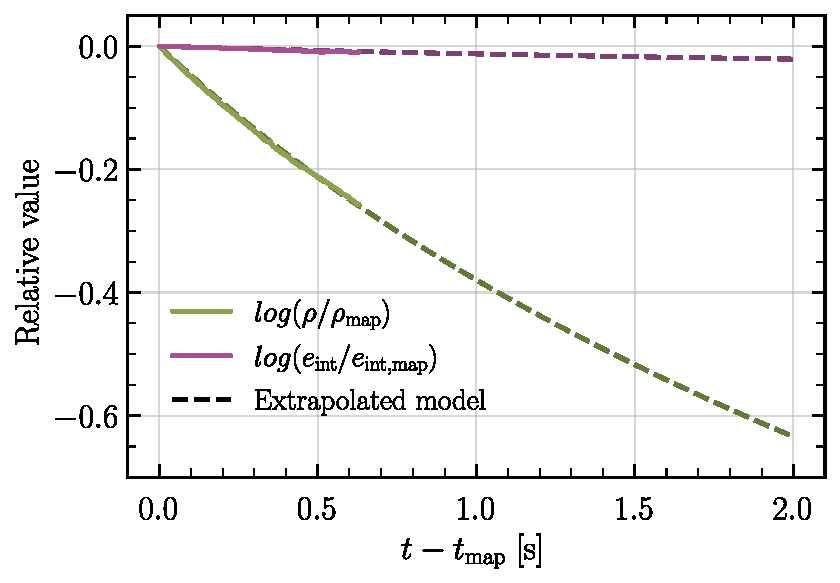
\includegraphics[width=0.75\linewidth]{figures/fit.pdf}
    \caption{Time-dependent behaviour of the neutrino-driven wind density \(\rho\), and internal energy \(e_\mathrm{int}\), from time of mapping \(t_\mathrm{map}\) at \(500\units{km}\), normalised to their mapping values, obtained from the initial 1D simulation of the z9.6 progenitor (solid lines) and extrapolated to later times using the best-fit power-law indices (dashed lines).}
    \label{fig:fit_1d}
\end{figure}

The composition of the ejecta is described by the two quantities \(\bar{\mathcal{A}}\) and \(\bar{\mathcal{Z}} = \bar{\mathcal{A}}Y_e\), and is fixed to represent a composition equivalent to that of alpha particles, therefore \(\bar{\mathcal{A}} = 4\) and \(\bar{\mathcal{Z}} = 2\). This is a somewhat average value, and does not impact considerably our simulations. However, if we were interested in the nucleosynthesis and the actual composition of the neutrino-heated ejecta, we would do so using a nuclear network, and would need to use appropriate values of \(\bar{\mathcal{A}}\), \(\bar{\mathcal{Z}}\) and \(Y_e\).

\subsection{Inflow condition: black hole} \label{sec:bdry_in}

What is referred to as the \emph{diagnostic explosion energy} is defined as the integral of the total energy density (i.e. kinetic, internal and gravitational) in the post-shock region, over volume elements where this quantity is positive. In other words, it is the energy contained in all the material that is unbound from the star. If the neutrino wind is strong enough, we expect an injection of energy to the explosion, as material is accelerated outwards by the wind and escapes the gravitational pull of the neutron star. After a few tens of seconds, once the wind has weakened, due to the drop in density and internal energy, the explosion energy saturates. At this point, we assume the neutrino wind to have little impact on the overall evolution of the explosion. Therefore, the outflow boundary condition is replaced with an inflow boundary condition. This new boundary condition effectively acts like a black hole, although it does not physically correspond to one, in which material falls but is not ejected. This condition is initially set at time \(t_\mathrm{hole}\), and at the same radius as the outflow condition, but expands at a velocity of \(100\units{km/s}\), further relaxing the time step as the boundary goes to larger and larger radii. The shock wave has already evolved very far from the core, and the ejected material has been accelerated to much higher velocities, so that the expansion of the boundary in no way affects the explosion energy.

\section{Implementation details}

To conclude this chapter, we give in this section some additional details on the usage of the \flash\ code, the implementation and internal behaviour of the inner boundary conditions, as well as some other considerations that we must have in order to run the simulations.

\subsection{Mapping procedure} \label{sec:mapping}

The progenitor models are provided in the form of 1D profiles, extending from the centre of the star to its surface, and give values of essential quantities (density, temperature, pressure, velocity, electron fraction, etc.) at different radii. When initialising a simulation, \flash\ reads the content of this model, creates a grid covering all radii, and fills each cells with values interpolated from the 1D profile. It is then possible to initialise a simulation on a reduced domain, only containing the central part of the star, by excluding the outer part of the progenitor's profile, as is done in the case of the initial simulations. When we wish to reintroduce the outer region to perform long-term simulations, we do so in 1D by simply appending this region of the progenitor's profile to the evolved profile of the simulation, and restarting \flash\ using the resulting, extended profile. \flash\ is then capable of determining the values of \(\rho_\mathrm{map}\), \(e_\mathrm{int,map}\) and \(v_\mathrm{wind}\) by evaluating the profile at the inner boundary, i.e \(500\units{km}\). In 2D, this procedure is more complex. We start by creating a 1D profile from a spherical average of the evolved, initial simulation to which we append the outer region of the progenitor's profile, such as in the 1D case. We then let \flash\ initialise a new 2D grid for the long-term simulation using the resulting profile, but without evolving it. It normally extracts values for the density, internal energy, and velocity for the neutrino wind from this spherically averaged profile, and initialises the inner boundary condition on the new 2D grid. This new grid now contains the outer region of the progenitor with the initialised inner boundary corresponding to the neutrino wind, but a spherical average of the initial simulation in the middle region. Using an external tool pipeline, we then remap the evolved 2D grid of the reduced domain from the initial simulation onto the new 2D grid, excluding the inner region that now contains the neutrino wind. The result is a 2D grid of the complete domain, containing the neutrino wind at its centre, the evolved region from the initial simulation at \(t_\mathrm{map}\), and the outer part of the progenitor, that can now be evolved to late times using \flash.

\subsection{Inner boundary structure} \label{sec:bdry_structure}

In principle, we want our boundary condition to be modelled as the surface of a region excised from the simulation, on which we prescribe values for the density, internal energy and velocity, constraining the hydrodynamical evolution of the adjacent cells. However, our version of \flash\ does not model our inner boundary condition in this way. Because \flash\ uses a Cartesian grid in 2D and 3D, our spherical inner boundary is not a smooth surface, but rather resembles a \emph{voxelised} structure made of square cells, not very suitable for such a description of a boundary condition. But more importantly, this would violate conservation, as mass and energy would be created and injected in the simulation from this surface. Consequently, the cells within the region inside the inner boundary, that we commonly refer to as \emph{the hole}, are still evolved normally, but \flash\ calls a routine after each time step that lets us adjust the conditions within these cells to match the desired state of our inner boundary. As a remark, the conditions inside the hole are still much more gentle than in the PNS, and this is sufficient to drastically reduce the resolution required in this region, so that the cost of evolving these inner cells is almost negligible. Any deviation from the expected mass in the cells within the inner region is then corrected using the mass contained in the point mass, and therefore preserves conservation in the system. Moreover, this means that mass can still accrete onto the boundary. The accreted mass would then be added to the point mass, and it becomes possible to follow the evolution of accretion on the central region at late times.

We note however that, because the cells in the inner region are still evolved, for the inner boundary condition to have the expected influence on the outside region, we must ensure that pressure support is kept inside the boundary. We do this by prescribing a power-law radial profile to the density and internal energy in order to have approximate hydrostatic equilibrium inside the hole. This is further discussed in \Cref{chap:results}.

\subsection{Point mass correction} \label{sec:pm_correction}

The \flash\ code is a Newtonian hydrodynamics code, which implies that the baryonic mass in the system is conserved during the simulation, but the neutrinos take out a non-negligible fraction of the total energy of the PNS, reducing the gravitational mass. This is taken in account in the code during the calculation of the effective gravitational potential mentioned earlier (Case A of \citealt{Marek2006}). However, this is not possible after mapping as we have placed all the mass, including the PNS, within the inner boundary inside a point mass. Thus, we must add a correction to the point mass at time of mapping to account for the loss of gravitational mass from the neutrino emission. This correction is calculated using the following expression:
\begin{equation}
    \Delta M = \frac{1}{c^2} \int_0^{t_\mathrm{map}} \left( L_{\nu_e} + L_{\bar{\nu_e}} + 4 L_{x} \right) \upd[t] \punct{,}
\end{equation}

where \(c\) is the speed of light, \(L_{\nu_e}\) and \(L_{\bar{\nu_e}}\) are the electron neutrino and antineutrino luminosities, and \(L_{x}\) is the heavy-lepton neutrino luminosity, which is multiplied by four, for each flavour of heavy-lepton neutrino (i.e. \(\mu\) and \(\tau\) neutrinos and antineutrinos). The value of this correction is given in \Cref{tab:pm_correction} for each simulation, and subtracted from the point mass at time of mapping.

\begin{table}[ht!]
\begin{threeparttable}
    \caption{Point-mass corrections for each simulation.}
    \label{tab:pm_correction}
    \centering
    \setstretch{1.2}
    \begin{tabular*}{\columnwidth}{c|@{\extracolsep{\stretch{1}}}*{4}{c}@{}}
         \hline
         \hline
         Simulation & z96 & s12hf1p0 & s12hf1p5 & s12hf2p0 \\
         Point mass correction [g] & \(1.032 \cdot 10^{32}\) & \(1.363 \cdot 10^{32}\) & \(1.226 \cdot 10^{32}\) & \(1.169 \cdot 10^{32}\) \\ \hline
    \end{tabular*}
\end{threeparttable}
\end{table}


\mainchapter{Results}{0.6}{But I am not so bold as to think that things cannot take place differently from the way I have specified.}{Anonymous} \label{chap:results}

%----------------------------------------%
% Results
%----------------------------------------%

This thesis revolves around the implementation of a new inner boundary condition into the \flash\ code. Accordingly, much of the work involved an iterative process of trials and errors, where the implementation was tested with various parametrisations, and the results were carefully analysed in order to improve or correct the code. Beginning with the 1D simulations of the z9.6 progenitor, we present the quantities we analysed, what was expected from the outcome of the simulations, and the solutions we have developed to improve the results. We then present the 2D simulations of the s12 progenitor, where we address the impact of different wind velocities on the evolution.

\section{1D simulations \& testing} \label{sec:results_1d}

The simplest way to begin is with a one-dimensional simulation. It is easy to learn and understand the essential features of CCSNe simulations from the profiles of a 1D simulation. In addition, it is relatively cheap to perform, and the implementation can more easily be tested. However, the neutrino-driven mechanism generally fails to produce explosions in spherical symmetry because it cannot capture the effects of non-spherically symmetric phenomena, such as turbulence and instabilities, that would otherwise help shock revival. The z9.6 progenitor is one of the few low-mass progenitors known to successfully explode in 1D.

\clearpage

\subsection{Composition \& features} \label{sec:results_features}

To familiarise ourselves with the structure and features of the simulation, we begin by looking at profiles of the progenitor star at moment of collapse. \Cref{fig:z96_composition} shows the shell structure at the centre of the star, where we can clearly identify the iron core, extending to \(1.1 \cdot 10^8\units{cm}\), as well as the composition interfaces between the silicon and carbon+oxygen layers (Si/C+O) at \(1.45 \cdot 10^8\units{cm}\), and between the carbon+oxygen and the helium layers (C+O/He) at \(6.7 \cdot 10^8\units{cm}\). The He/H composition interface, located at a radius of \(1.4 \cdot 10^{12}\units{cm}\), does not appear on \Cref{fig:z96_composition}.

\begin{figure}[ht!]
    \centering
    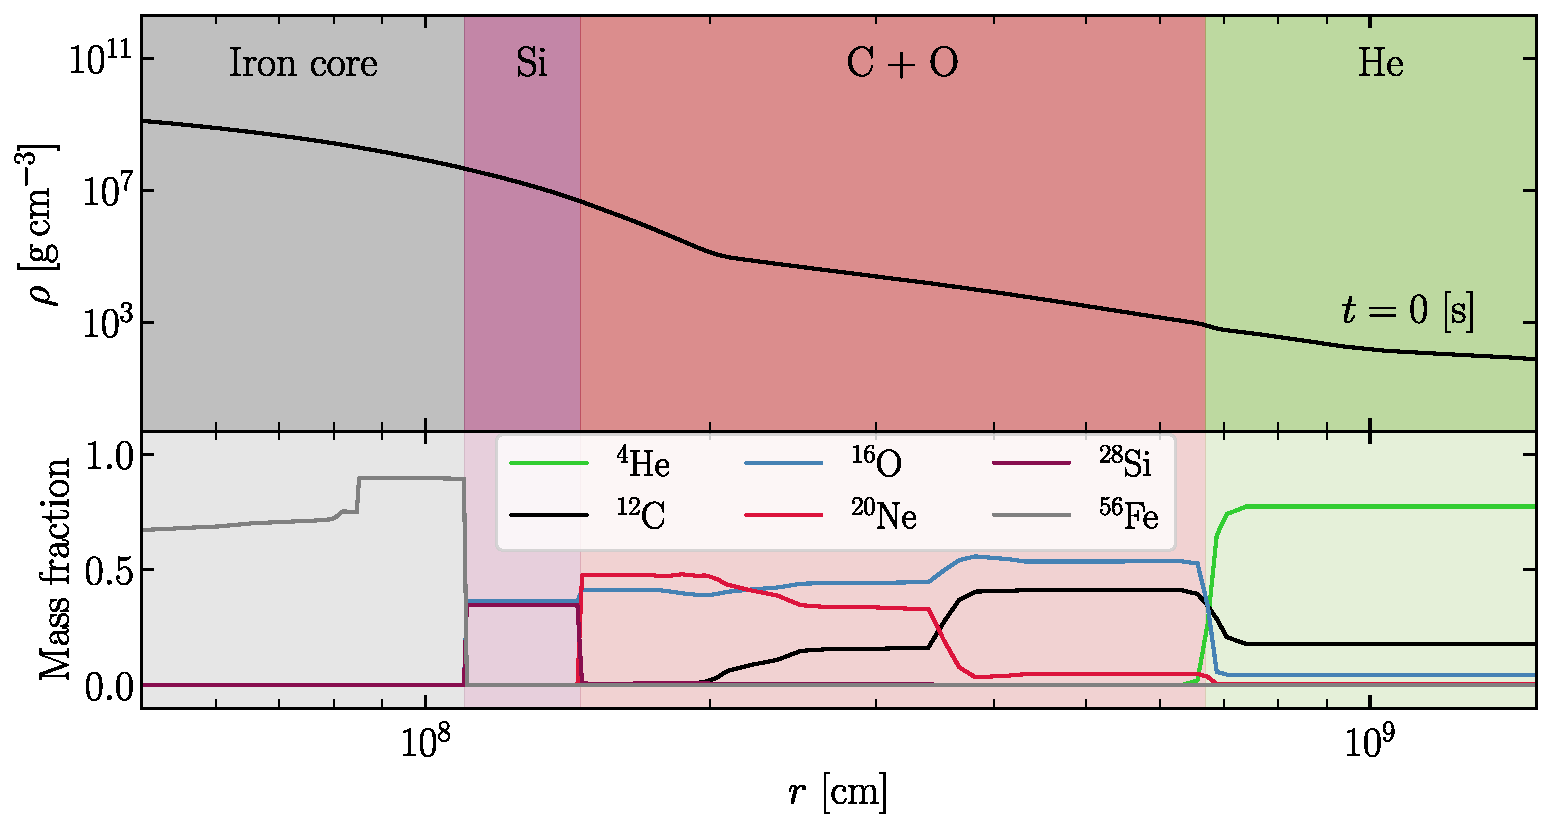
\includegraphics[width=1.0\linewidth]{figures/composition_1d.pdf}
    \caption{1D profile of the density \(\rho\) and the mass fractions of the main elements present in the depicted region, showing the core structure of the z9.6 progenitor at moment of collapse.}
    \label{fig:z96_composition}
\end{figure}

We then look at an evolved state of the simulation, at time of mapping \(t_\mathrm{map} = 1.6\units{s}\). At this point, the core has collapsed into a PNS, and the shock has propagated to a few thousand kilometres. \Cref{fig:z96_features} highlights the region of nuclear density corresponding to the location of the PNS, as well the \emph{forward shock} and the \emph{reverse shock}. The forward shock is the initial shock launched at time of bounce, which has been revived by neutrino heating and sweeps up the material in the outer layers of the star. The reverse shock propagates inward into the inner ejecta. As shown in \Cref{fig:z96_features}, the reverse shock is formed due to the ejecta being accelerated by the neutrino wind to supersonic speeds, and entering in contact with the shocked material behind the forward shock, causing a sharp drop in velocity and heating the material.

\begin{figure}[ht!]
    \centering
    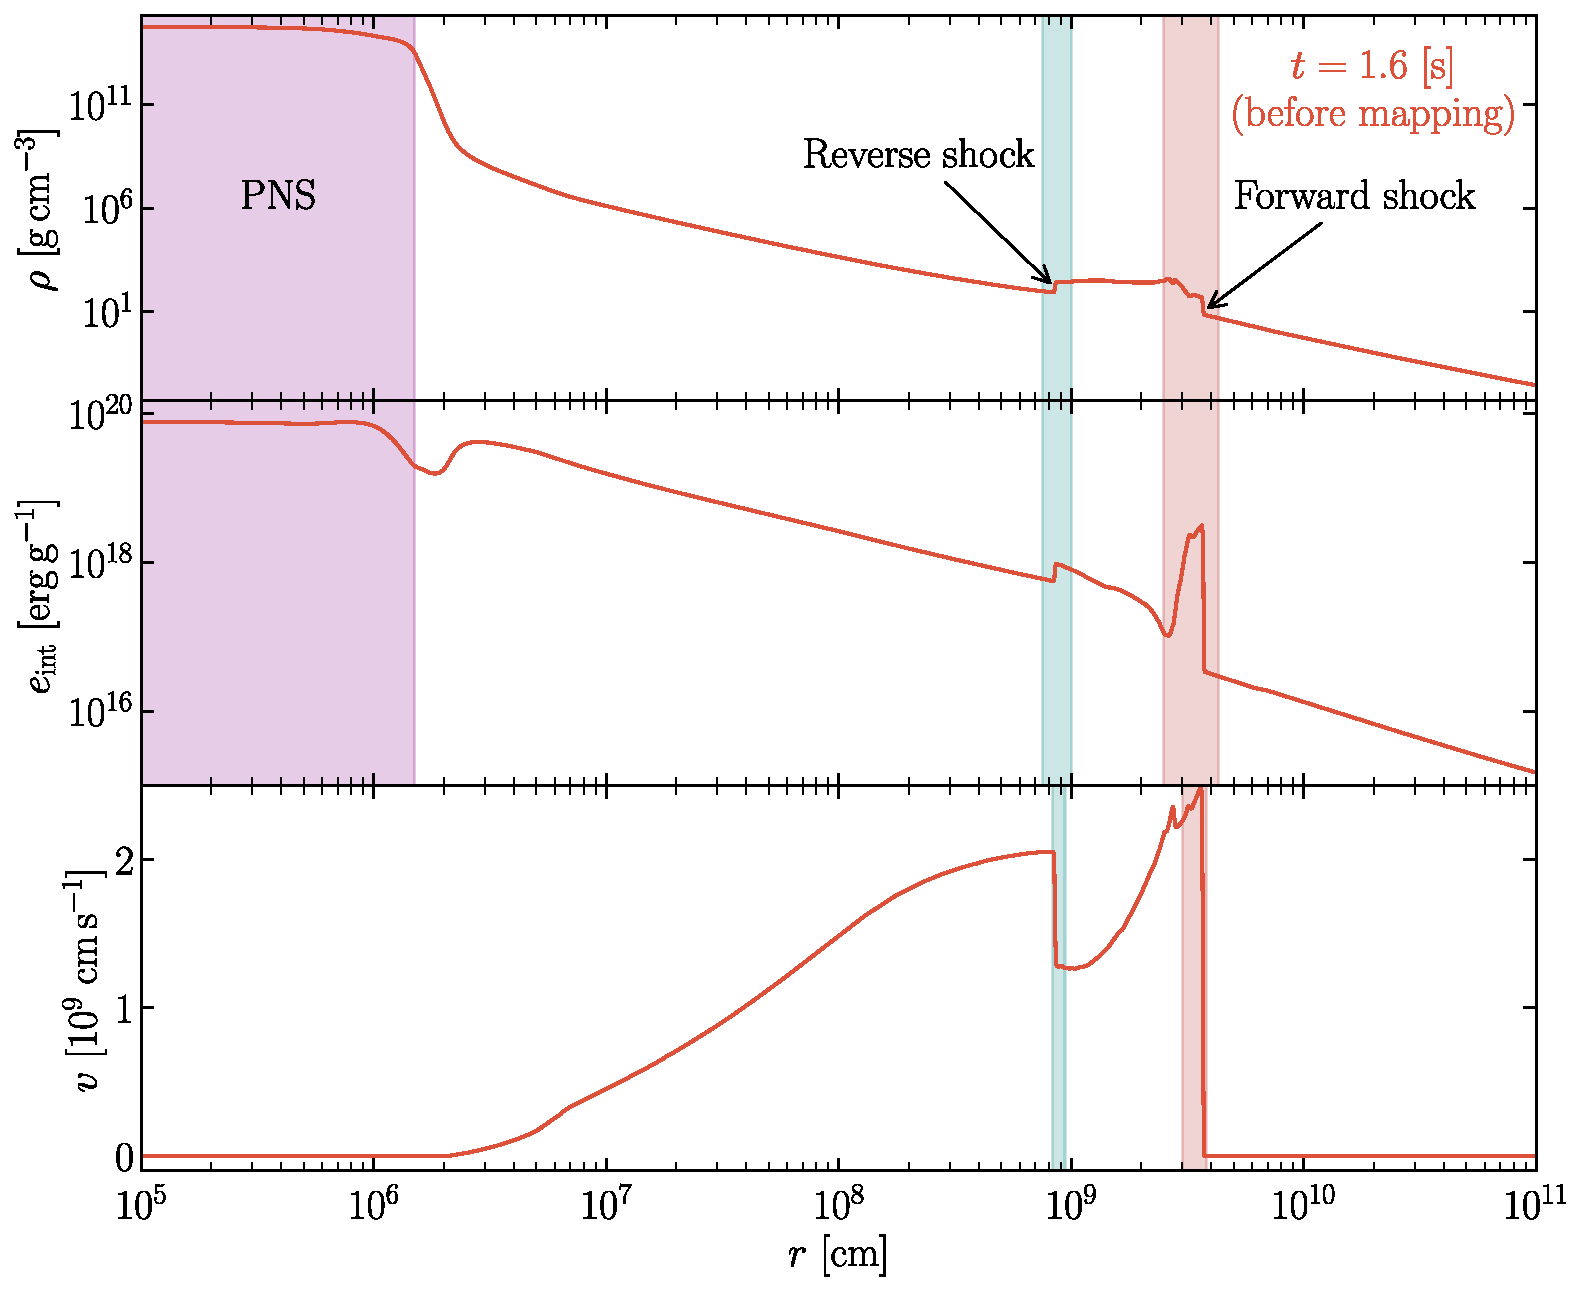
\includegraphics[width=1.0\linewidth]{figures/features_1d.pdf}
    \caption{1D profiles of the density \(\rho\), internal energy \(e_\mathrm{int}\), and velocity \(v\) for the initial simulation at time of mapping \(t_\mathrm{map} = 1.6\units{s}\) of the z9.6 progenitor. The region of nuclear density corresponding to the PNS is shown (purple region), as well as the discontinuities in thermodynamical state associated with the forward and reverse shocks (red and blue regions).}
    \label{fig:z96_features}
\end{figure}

\clearpage

\subsection{Spatial gradient} \label{sec:results_gradient}

The first implementation of the neutrino wind boundary condition prescribed constant values of density and internal energy inside the hole, following the model presented in \Cref{sec:bdry_out}. The velocity is kept constant at the inner boundary, but declines as \(\sqrt{r}\) inside the hole. This is done to prevent instabilities near \(r=0\), as the cells are still evolved in this region. Conveniently, this approximately matches the shape of the velocity profile from the initial 1D simulation near the inner boundary. The left panel of \Cref{fig:compare_grad} shows the result of a simulation ran until \(12\units{s}\) post-collapse with this first implementation. We see that the density profile outside the boundary matches the evolution of the initial simulation at \(1.6\units{s}\) and \(2.2\units{s}\). However, we note a rapid loss of velocity at the inner boundary that propagates to the reverse shock. This is not a desirable behaviour and could have a significant influence on the long-term evolution of the reverse shock. To attenuate this effect, we instead prescribe a spatial gradient profile to the density and internal energy inside the hole, that we express as power-laws in the same way as we did the time evolution presented in \Cref{sec:bdry_out}, but replacing the time variables with the radius. To find an adequate power-law index, we fit the density and internal energy profiles of the initial simulation in the same way as we fit the power-law index for the time evolution, again replacing the time variable with the radius. This would result in infinitely large density and internal energy near \(r=0\), defeating the purpose of the boundary condition. However, since we put the mass within the hole in a point mass, \flash\ does not compute the gravitational potential beyond a certain radius inside the hole, as this would result in a gravitational singularity at \(r=0\). This softening radius, \(r_\mathrm{soft}\), is set at \(250\units{km}\). To achieve approximate hydrostatic equilibrium, we only need to prescribe our spatial gradient between this radius and the inner boundary. The right panel of \Cref{fig:compare_grad} shows the results of this new implementation. We still note a discontinuity in the velocity profile at the inner boundary due to numerical issues, however, we see that the material at the reverse shock is still correctly accelerated and that the profile matches better with the initial simulation at \(2.2\units{s}\).

\begin{figure}[ht!]
    \centering
    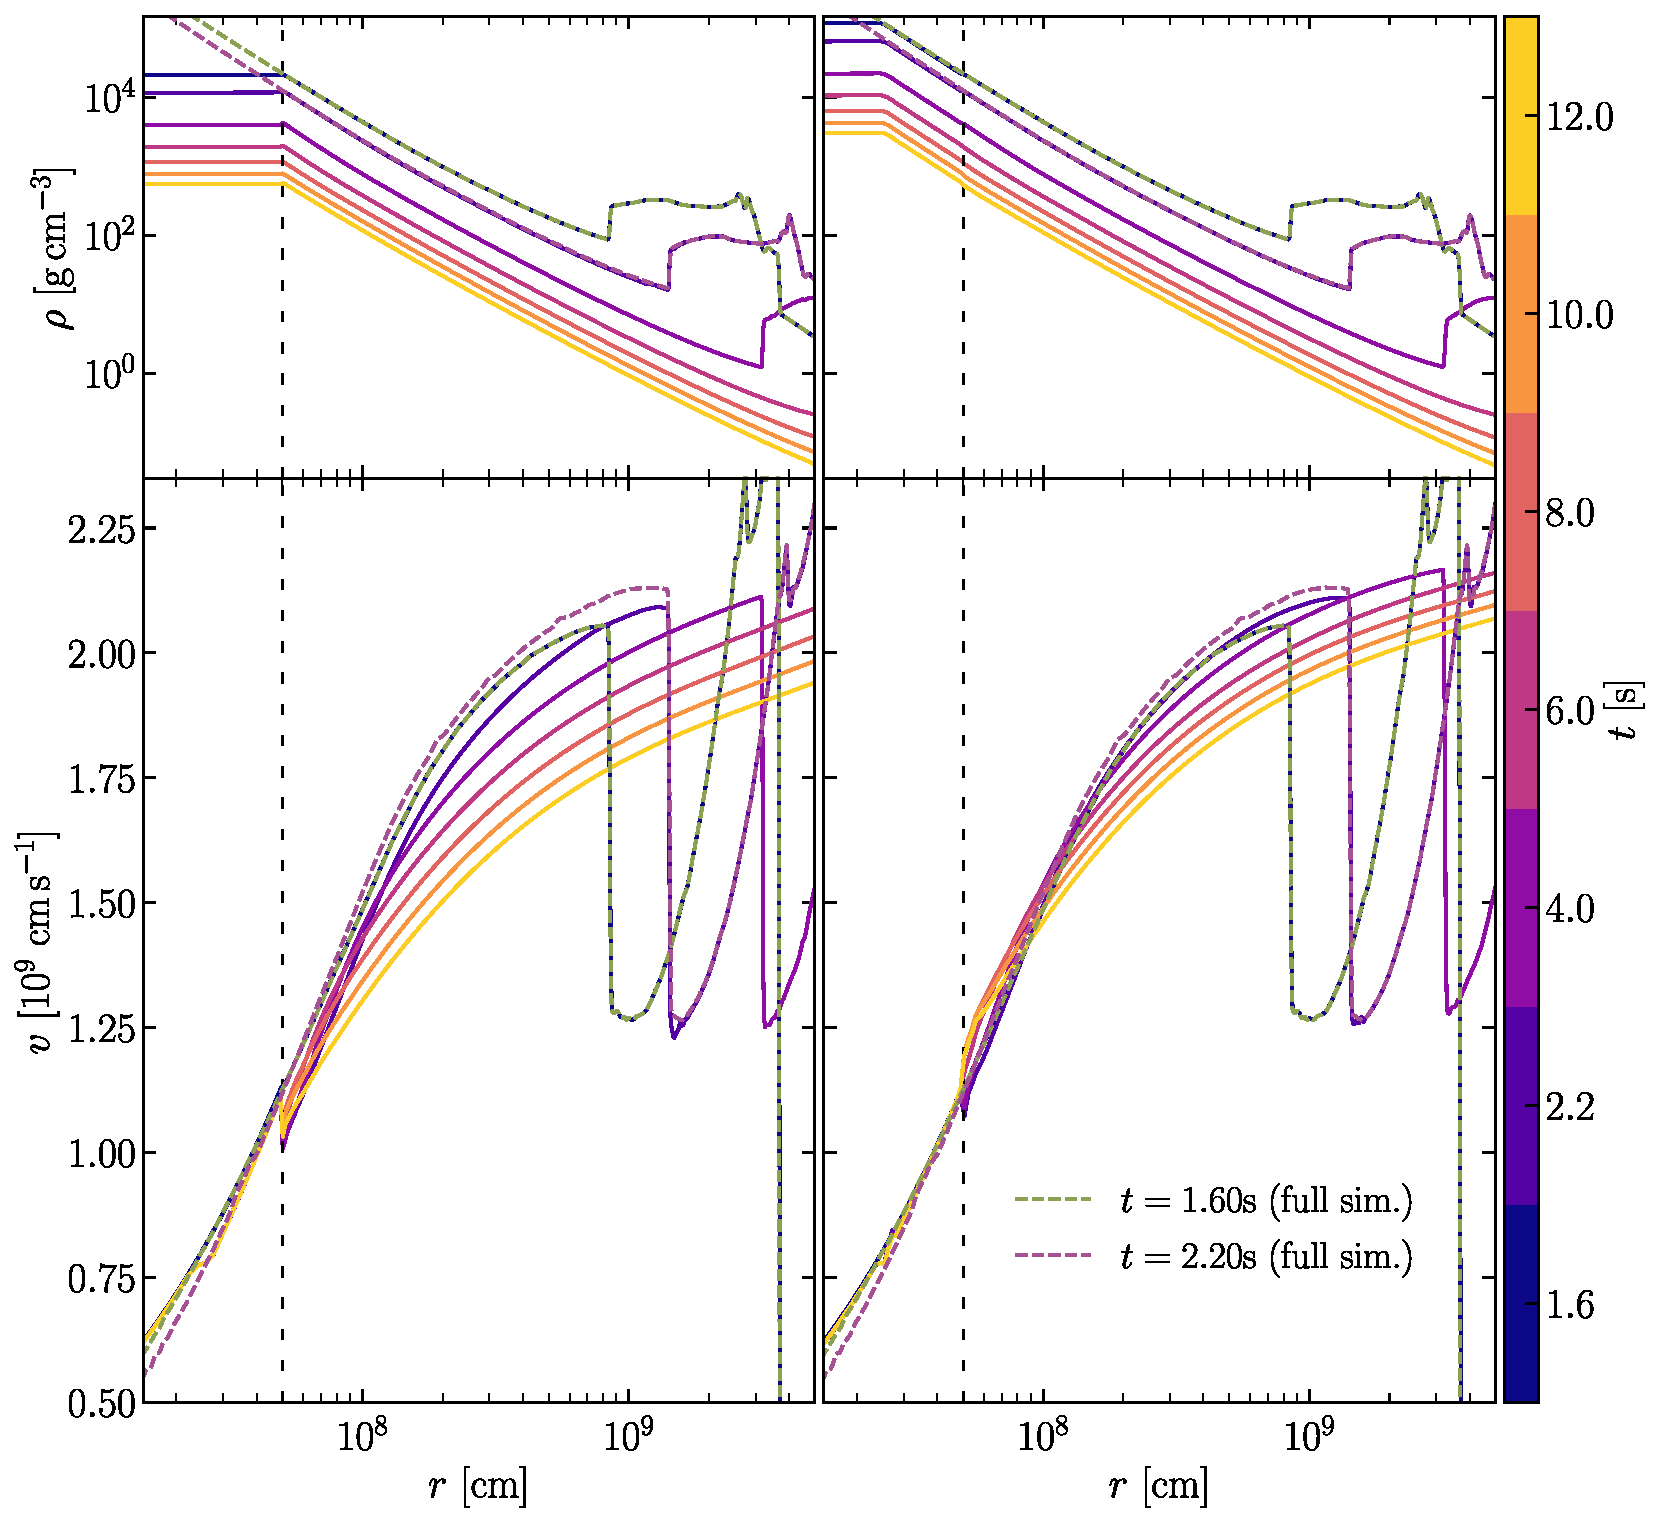
\includegraphics[width=1.0\linewidth]{figures/compare_grad.pdf}
    \caption{Comparison of the time evolution of the density and velocity near the inner boundary between a simulation without (left panel) and with approximate hydrostatic equilibrium inside the hole (right panel). The time evolution of the long term simulation (solid lines) is shown from time of mapping \(t_\mathrm{map} = 1.6\units{s}\) to \(12\units{s}\), and compared with profiles from the initial simulation (dashed lines) at \(1.6\units{s}\) and \(2.2\units{s}\).}
    \label{fig:compare_grad}
\end{figure}

\clearpage

\subsection{Long-term profiles}

We now look at the final results of the long-term simulation for the z9.6 progenitor. \Cref{fig:short_1d} shows a series of profiles of the density, internal energy and velocity from time of mapping to \(10\units{s}\) after collapse, on which we see the expansion of the forward shock, as well as the slower expansion of the reverse shock.

\begin{figure}[ht!]
    \centering
    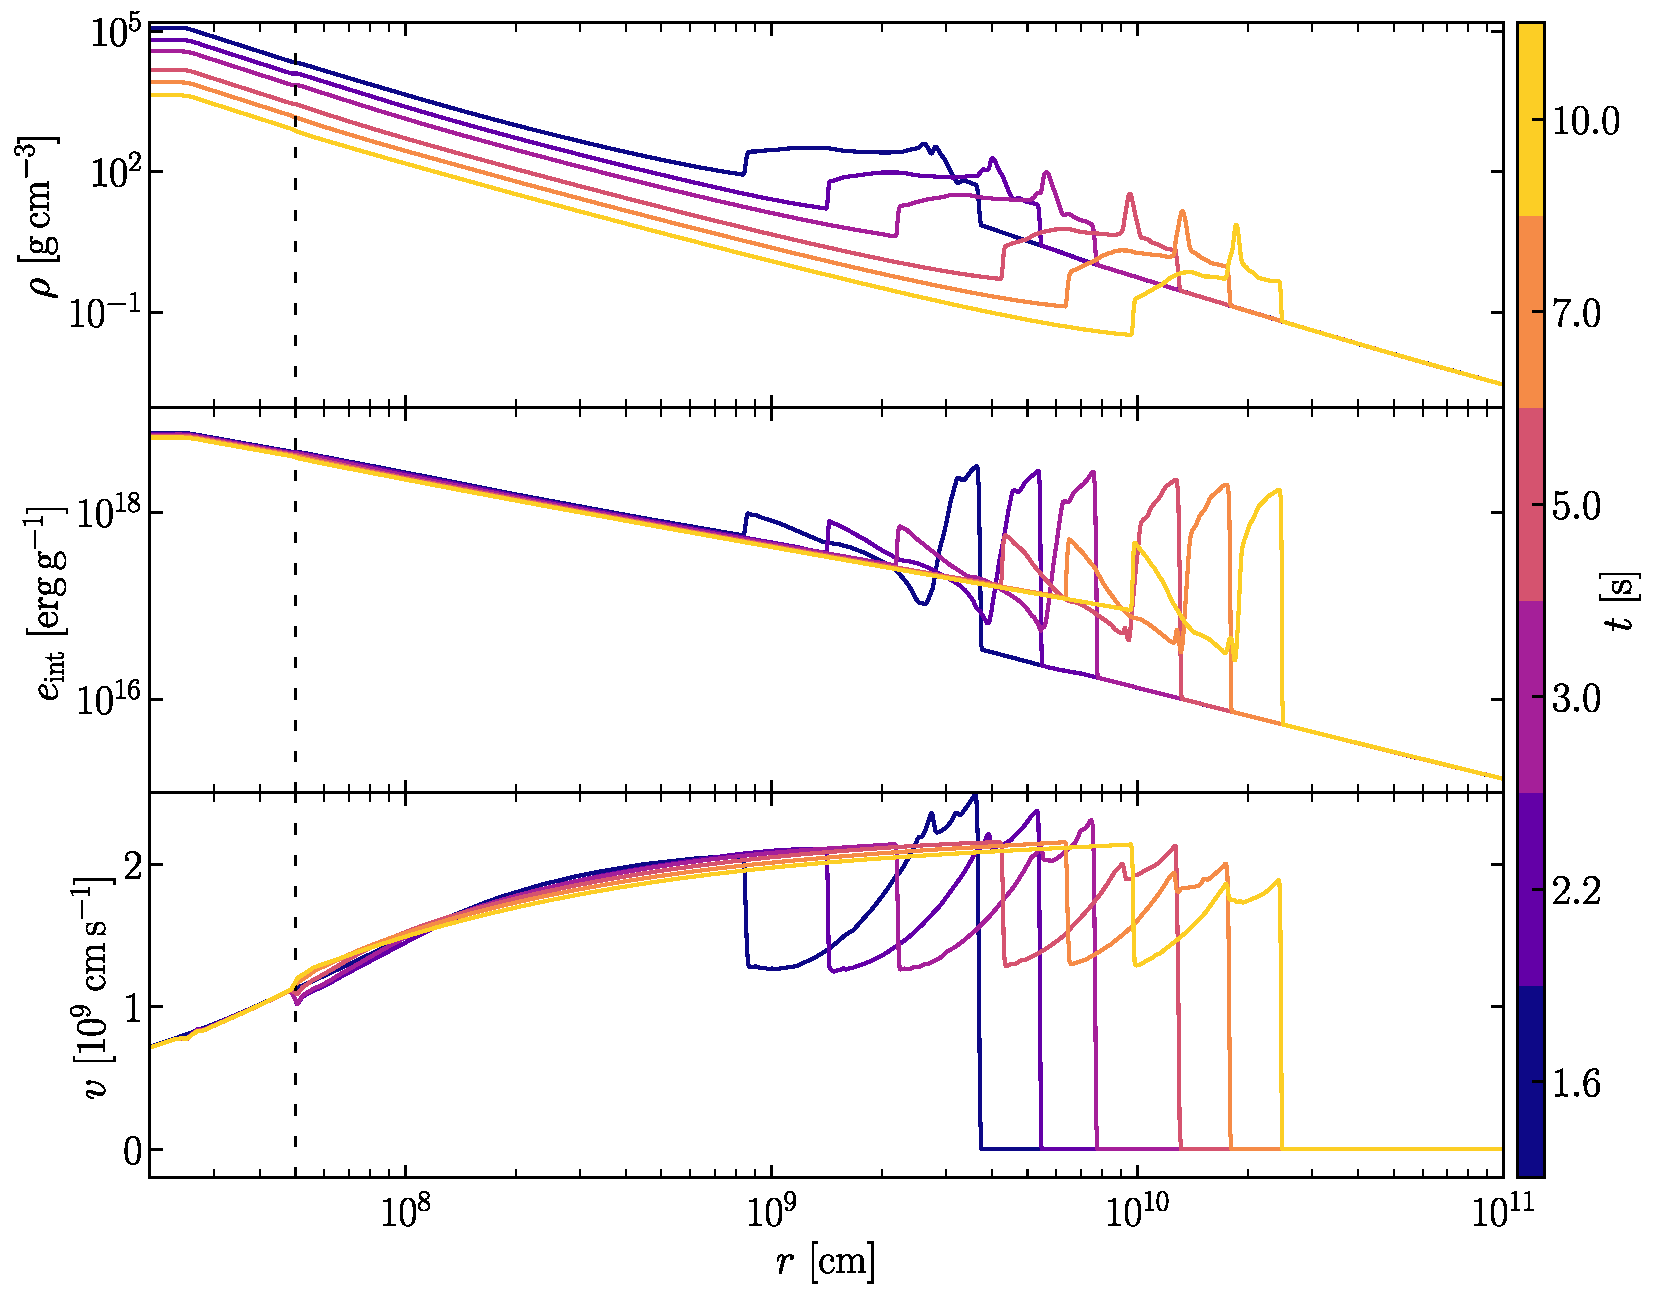
\includegraphics[width=1.0\linewidth]{figures/short_1d.pdf}
    \caption{1D profiles of the density \(\rho\), internal energy \(e_\mathrm{int}\) and velocity \(v\) from time of mapping \(t_\mathrm{map}\) to \(10\units{s}\) post-collapse. The neutrino wind boundary condition is used during this time, with the inner boundary located at \(r=500\units{km}\) (vertical black dashed line).}
    \label{fig:short_1d}
\end{figure}

\Cref{fig:long_1d} shows profiles of the evolution until shock breakout. At \(20\units{s}\), the density of the wind has already dropped to \(\sim10^2\units{g/cm^3}\). At \(30\units{s}\), the neutrino wind is replaced with the inflow boundary condition described in \Cref{sec:bdry_in}, in which the density and internal energy at the boundary are set to a fraction (1\%) of their values directly outside the boundary, producing a discontinuity at the boundary and a flat profile inside the hole. The velocity is also set to zero. At \(\sim100\units{s}\), the boundary has expanded to a radius of \(\sim8\cdot10^8\units{cm}\), and the reverse shock, at \(\sim8\cdot10^{10}\units{cm}\), begins to recede. We note that the behaviour of the reverse shock is influenced by the introduction of the inflow boundary condition, which shuts off the ejecta and causes a loss of pressure support in the centre, and may cause it to recede earlier than it otherwise would have. Much later, at \(\sim20{,}000\units{s}\), the boundary has expanded to its maximum radius of \(2\cdot10^{11}\units{cm}\), and after \(\sim100{,}000\units{s}\), the forward shock has reached the outer boundary of the domain, indicating shock breakout.

\begin{figure}[ht!]
    \centering
    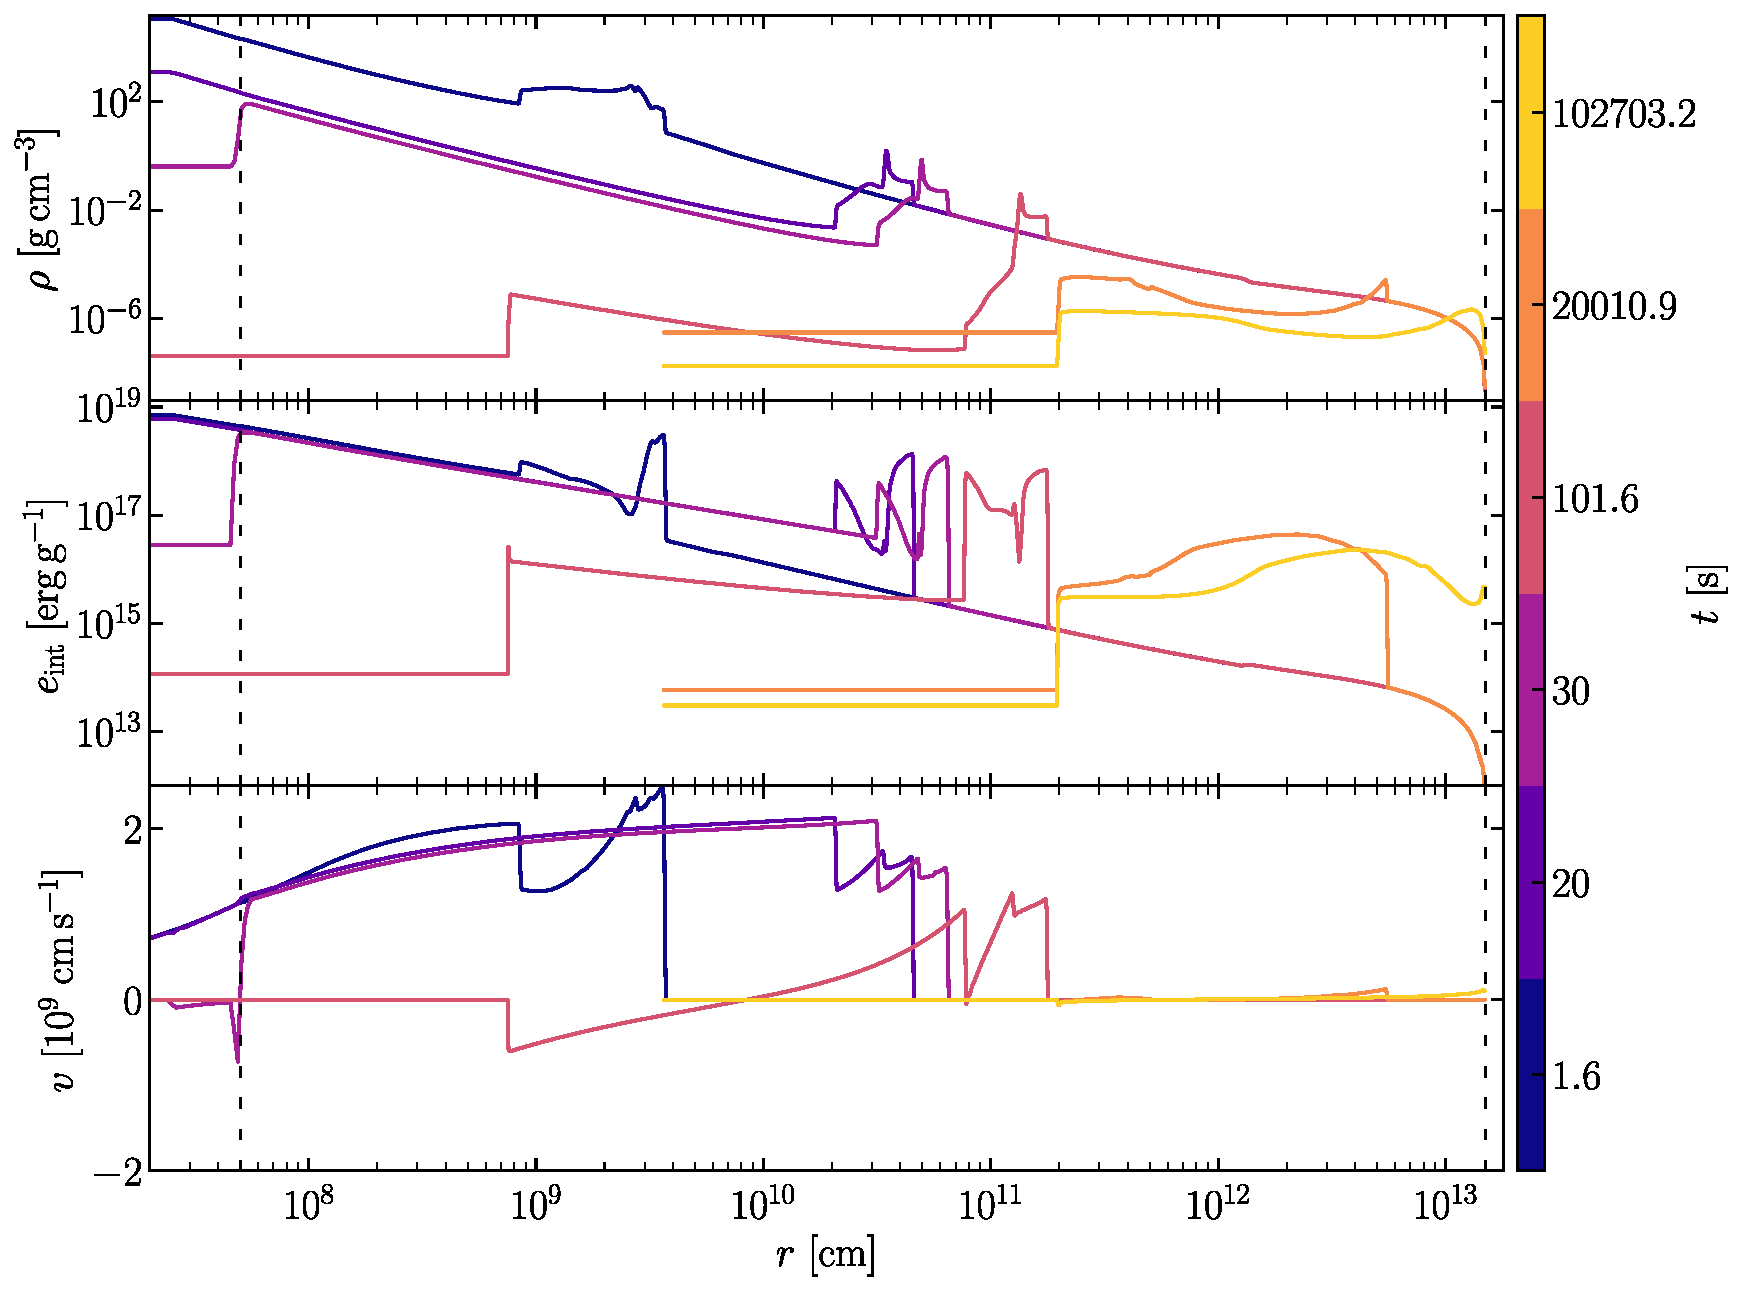
\includegraphics[width=1.0\linewidth]{figures/long_1d.pdf}
    \caption{1D profiles of the density \(\rho\), internal energy \(e_\mathrm{int}\) and velocity \(v\) from time of mapping \(t_\mathrm{map}\) to shock breakout from the stellar surface. The inner boundary for the neutrino wind is located at \(r=500\units{km}\). At \(t = 30\units{s}\), a sharp drop in density and internal energy at the inner boundary indicates the transition to the inflow boundary condition. The boundary of the inflow condition expands at \(100\units{km/s}\) until reaching a maximum radius of \(2 \cdot 10^{11}\units{cm}\) at about \(t=20{,}000\units{s}\). The shock reaches the surface of the star, at \(r=1.5 \cdot 10^{13}\units{cm}\), at a time of about \(100{,}000\units{s}\) post-collapse.}
    \label{fig:long_1d}
\end{figure}

\clearpage

\subsection{Shock propagation \& explosion energy}

In \Cref{fig:long_1d} we can see the velocity of the forward shock drop to very low values as it reaches the stellar surface. This is caused by density gradients in the stellar envelope. According to \cite{Sedov1959}, positive gradients of the \(\rho r^3\) profile will cause a deceleration of the shock wave, whereas negative gradients will accelerate it. This can be seen in \Cref{fig:shock_vel}, where we have plotted the \(\rho r^3\) profile and shock velocity against radius. The shock is originally rapidly accelerated to very high velocities, about \(35{,}000\units{km/s}\), as it escapes the iron core due to the steep, negative density gradient in the Si layer. It is then gradually decelerated after crossing the C+O/He interface to just a few \(100\units{km/s}\) as it reaches the stellar surface. We note that the shock velocity we have obtained is consistent with the 3D simulations of the z9.6 progenitor of \cite{Stockinger2020} as well as the multidimensional simulations of the same progenitor by \cite{Sandoval2021}.

\begin{figure}[ht!]
    \centering
    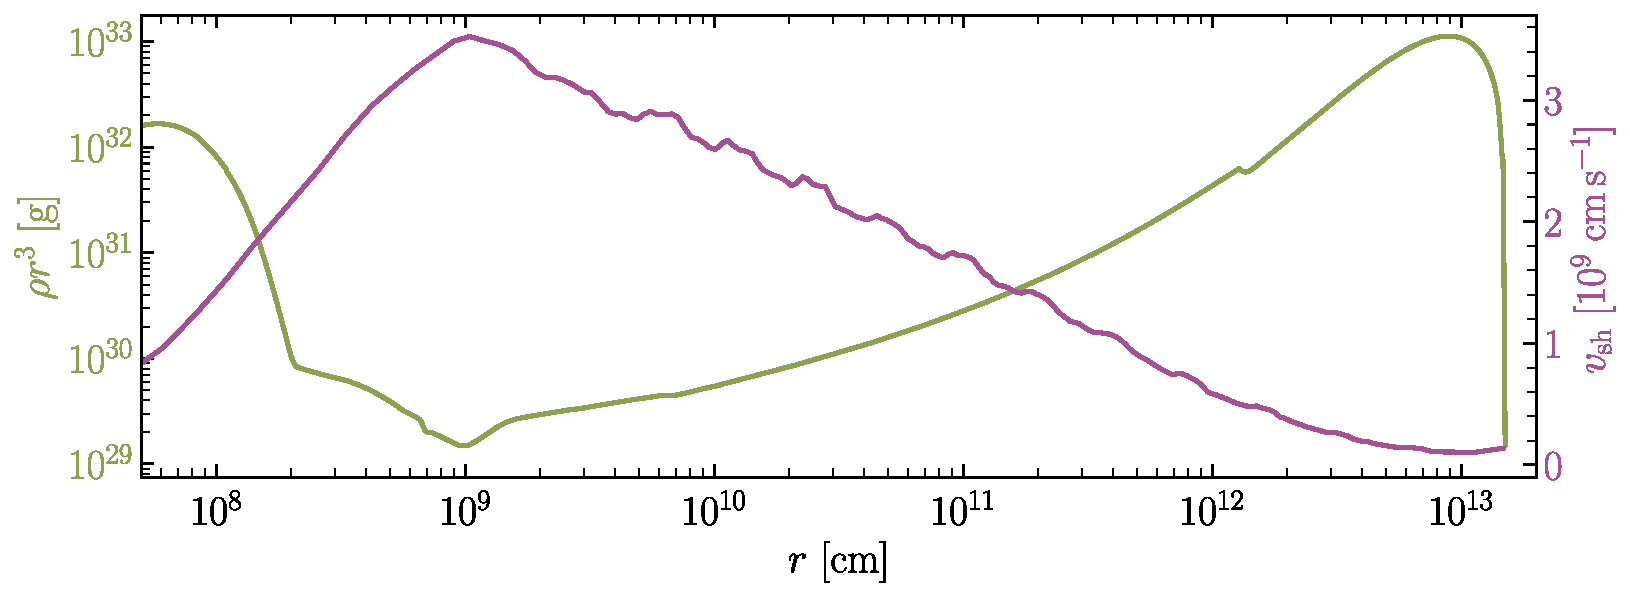
\includegraphics[width=1.0\linewidth]{figures/shock_vel.pdf}
    \caption{Shock velocity (right axis) and \(\rho r^3\) (left axis) radial profiles of z9.6 progenitor.}
    \label{fig:shock_vel}
\end{figure}

Lastly, \Cref{fig:quantities_1d} shows the shock radius, shock velocity and diagnostic explosion energy from \(0.4\units{s}\) to \(30\units{s}\) after collapse. This corresponds to a time slightly after shock revival, until the moment the neutrino wind is shut down and replaced with the inflow boundary condition. We note a smooth continuation of the shock radius and velocity between the data from the initial simulation, in green, and the long term simulation in purple, although the shock velocity is a little noisy. The diagnostic explosion energy shows a slight offset of \(\sim2\%\). This gap is due to different definitions of the diagnostic explosion energy and the need to account for the nuclear EoS before mapping, which is absent after mapping. We can however see an injection of energy of about \(3\%\) from the neutrino wind, resulting in an explosion of \(\sim0.1\units{B}\), where the \emph{Bethe} is defined as \(1\units{B} = 10^{51}\units{erg}\) \citep{Weinberg2006}.

\begin{figure}[ht!]
    \centering
    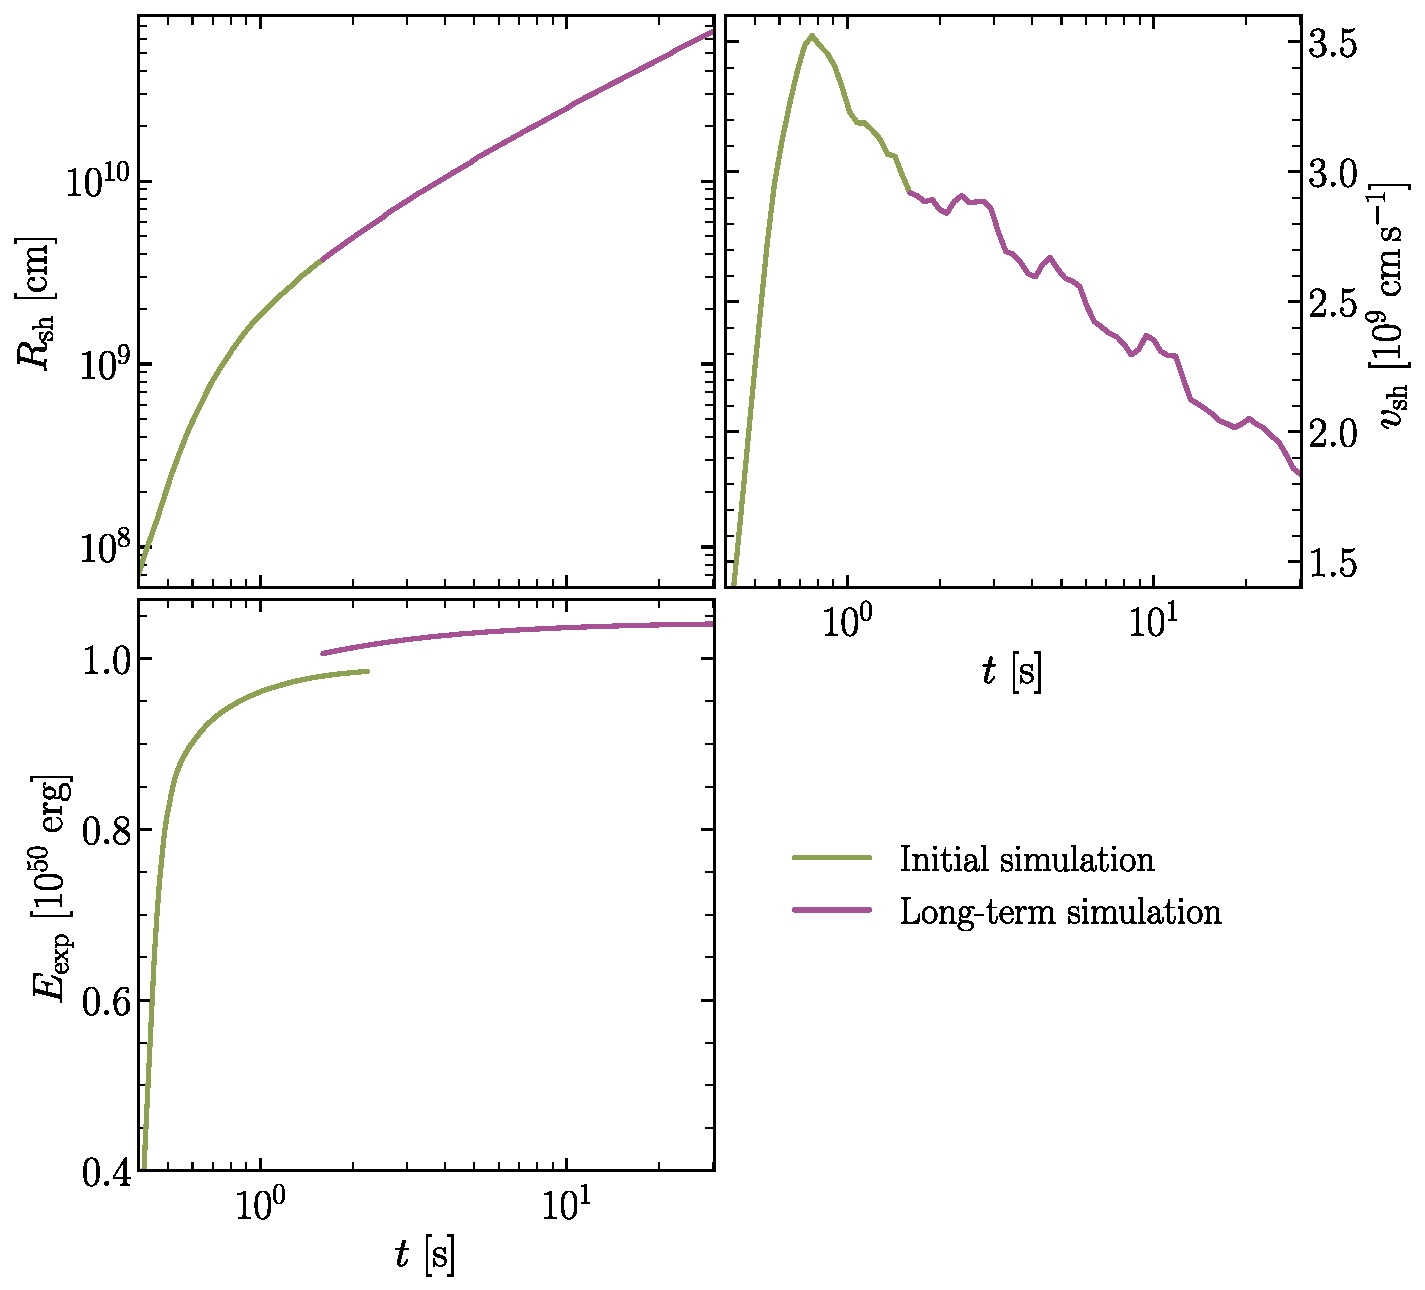
\includegraphics[width=0.9\linewidth]{figures/quantities_1d.pdf}
    \caption{Shock radius (top left), shock velocity (top right), and diagnostic explosion energy (bottom left) from \(0.4\units{s}\) to \(30\units{s}\) after collapse for the z9.6 progenitor. Before mapping, the results are taken from the initial simulation (green line), with a slight overlap with the long-term simulation (purple line) for the diagnostic explosion energy, as data from the initial simulation were available until \(2.2\units{s}\) after collapse.}
    \label{fig:quantities_1d}
\end{figure}

\clearpage

\section{2D simulations} \label{sec:results_2d}

We now look at the 2D simulations of the s12 progenitor. These simulations were run with different neutrino heating factors and wind velocities, as summarised in \Cref{tab:sim_params}.
%In addition, for each of the initial three simulations, with different heating factors, we have run another set of simulations using only the inflow boundary condition instead of the neutrino wind.

\subsection{Wind velocity}

For the 1D simulations, the condition of spherical symmetry forces the formation of a neutrino-driven wind after shock revival, and it is easy to map our neutrino wind condition using the value of the velocity from the profile of the initial simulation. In 2D however, asymmetrical phenomena such as convection and turbulence complicate this picture and can result in regions of accretion and ejection of material around the PNS, which does not map well with our spherically symmetric wind. For this reason, and as was discussed in \Cref{sec:lt_setup}, it was not possible to obtain a realistic wind velocity from the spherically averaged profile of the initial simulation. Consequently, we have decided to run simulations using different wind velocities to explore the impact of this parameter on the long-term evolution of the simulation.

The first two simulations involved the s12 progenitor with a heating factor \(f_\mathrm{heat} = 1.0\). One simulation was ran with a weak wind of \(10{,}000\units{km/s}\), and the other with a strong wind of \(28{,}000\units{km/s}\).

\Cref{fig:s12hf1p0_og} shows slices of the initial s12hf1p0 simulation, showing that at time of mapping \(t_\mathrm{map} = 1.0\units{s}\) the PNS was accreting matter from the north pole and equator, while driving a strong wind at the south pole, with velocities exceeding \(30{,}000\units{km/s}\). As a result, \Cref{fig:s12hf1p0_strong_slice} shows that, after mapping the inner boundary condition, the strong neutrino wind crashes against the still accreting material, launching a shock, as can be seen on the left panel. This shock does not completely extend to the south pole, where the wind was already strong in the initial simulation. The right panel of \Cref{fig:s12hf1p0_strong_slice} shows the continuing accretion of matter on the north pole, while the wind extends at the bottom to a radius of about \(1.2\cdot10^8\units{cm}\), where a termination shock forms around the central region.

\begin{figure}
    \centering
    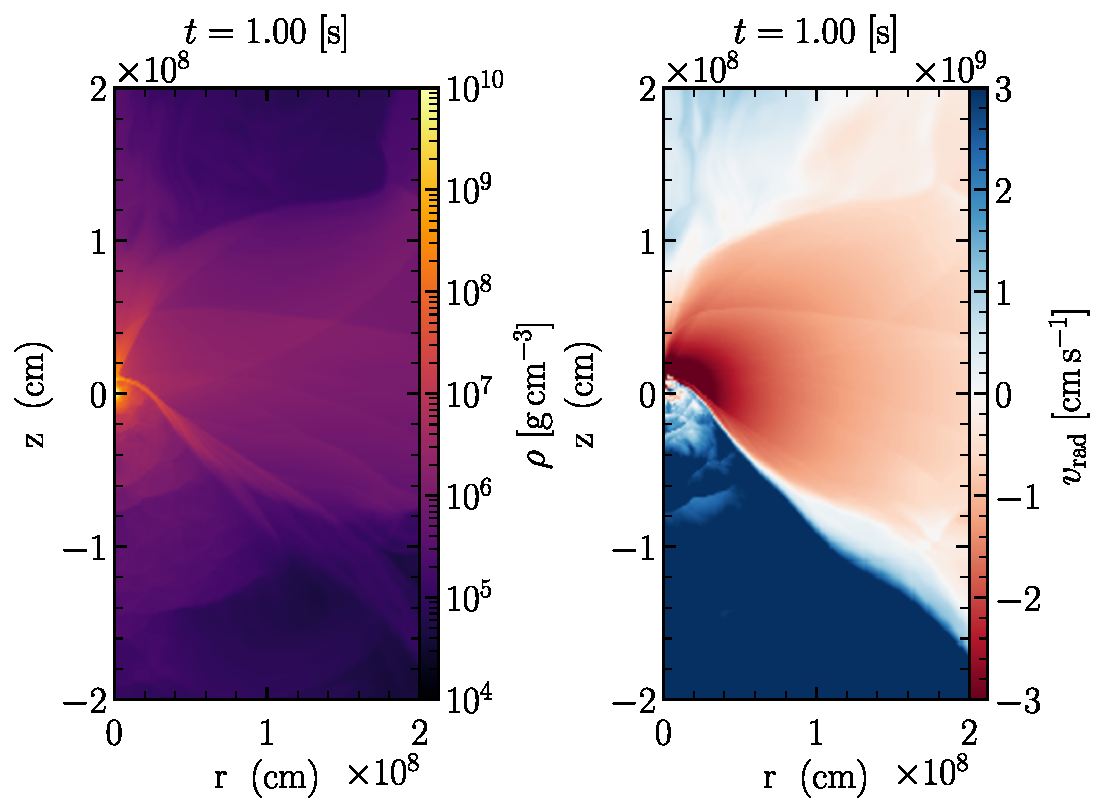
\includegraphics[width=1.0\linewidth]{figures/s12hf1p0_og.pdf}
    \caption{Slices of the initial s12hf1p0 simulation, showing density (left) and radial velocity (right) near the PNS at time of mapping.}
    \label{fig:s12hf1p0_og}
\end{figure}

\begin{figure}[ht!]
    \centering
    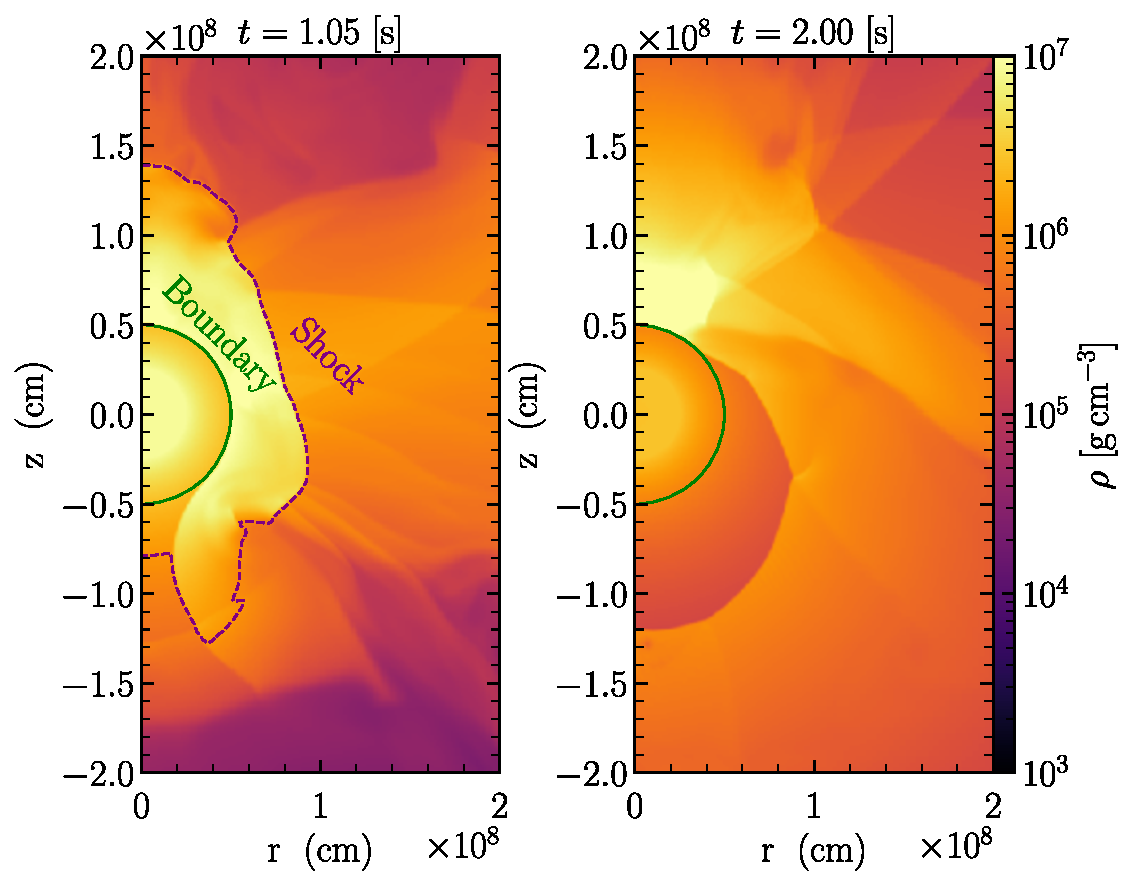
\includegraphics[width=1.0\linewidth]{figures/s12hf1p0_strong_slice_annot.pdf}
    \caption{Slices of the s12hf1p0\_w28e8 simulation, with a strong wind, at \(t=1.05\units{s}\) post-bounce (left) and \(t=2.0\units{s}\) post-bounce (right). A shock is formed (purple contour) by the introduction of the neutrino wind at the inner boundary (green contour).}
    \label{fig:s12hf1p0_strong_slice}
\end{figure}

\clearpage

In addition to the diagnostic explosion energy, it becomes interesting to look at the time evolution of the point mass in the 2D case. Whereas this quantity stayed mostly constant for the 1D simulation, that had no difficulties pushing material out, \Cref{fig:s12hf1p0_strong_quantities} shows a positive gradient of this quantity for the s12hf1p0\_w28e8 simulation, that accretes \(\sim0.1\sunmass\) over the first \(10\units{s}\) of evolution.

\begin{figure}[ht!]
    \centering
    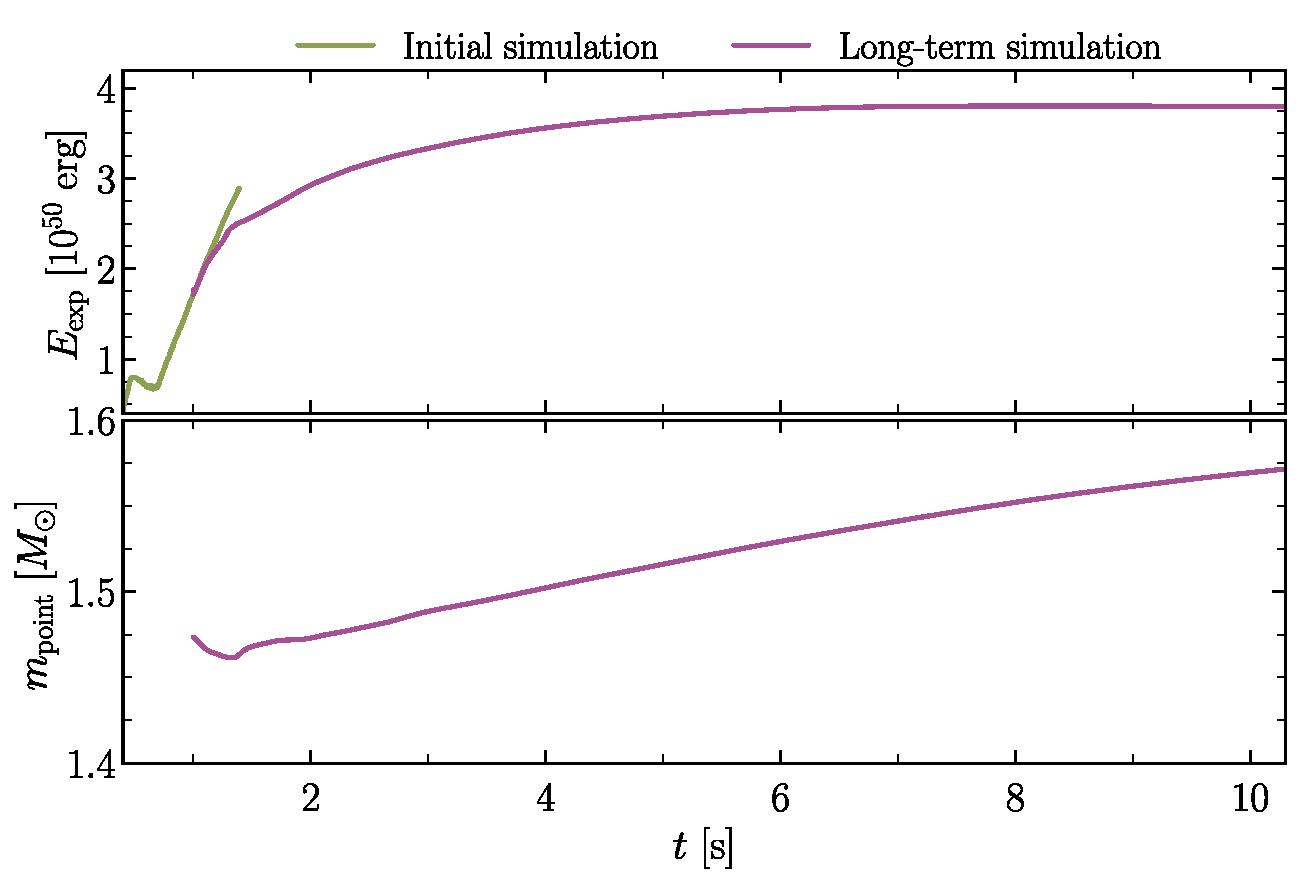
\includegraphics[width=0.9\linewidth]{figures/s12hf1p0_strong_quantities.pdf}
    \caption{Diagnostic explosion energy (top) and point mass (bottom) evolution from time of mapping at \(t_\mathrm{map} = 1.0 \units{s}\) to \(10\units{s}\) post-bounce for the s12hf1p0\_w28e8 simulation.}
    \label{fig:s12hf1p0_strong_quantities}
\end{figure}

We can compare these results with the weak-wind counterpart of this simulation, the s12hf1p0\_w10e8. This simulation uses a wind velocity similar to that of the 1D simulation of the z9.6 progenitor, but is too weak to drive any ejecta in the 2D simulation of the s12 progenitor. \Cref{fig:s12hf1p0_weak_slice} shows a similar view as \Cref{fig:s12hf1p0_strong_slice} for the s12hf1p0\_w10e8 simulation. We see that material keeps accreting on the inner boundary, but the wind is too weak to launch a shock such as for the s12hf1p0\_w28e8 simulation. In the same way, the wind fails to extend to larger radii and material falls back onto the inner region.

\begin{figure}[ht!]
    \centering
    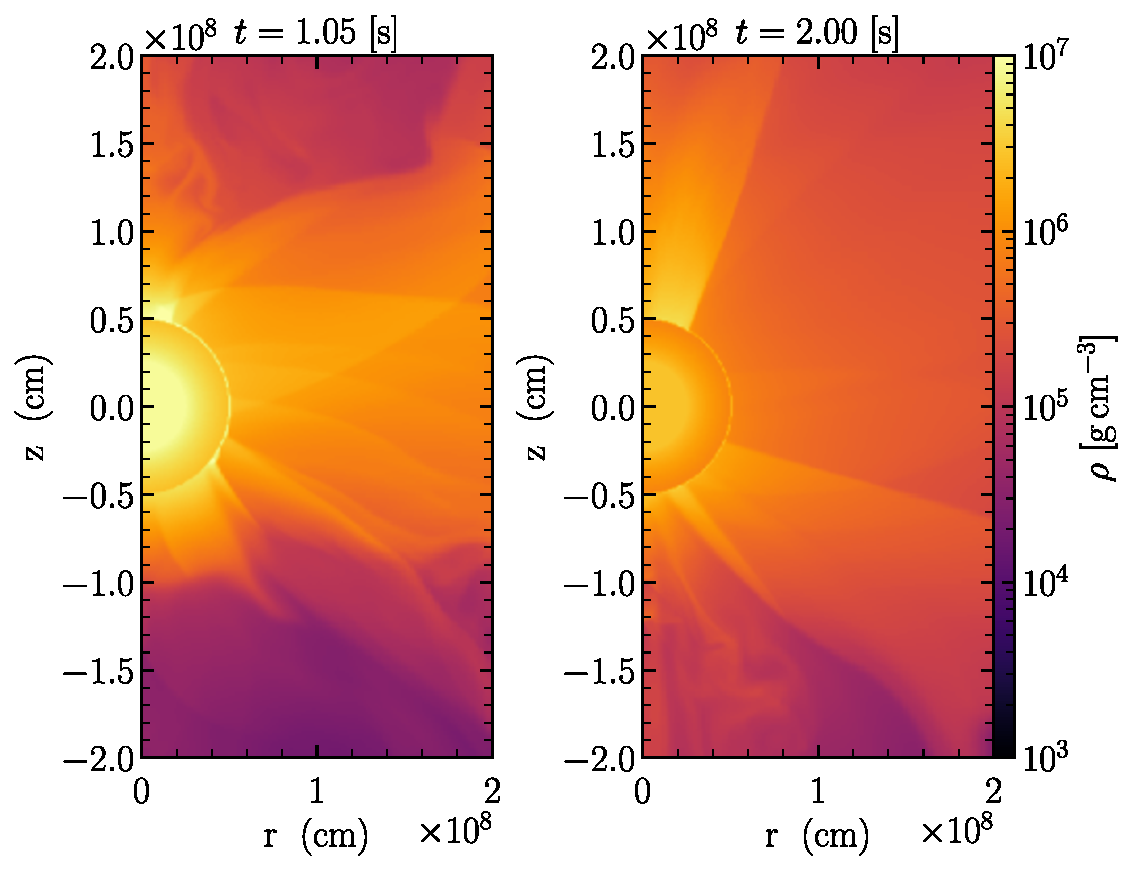
\includegraphics[width=1.0\linewidth]{figures/s12hf1p0_weak_slice.pdf}
    \caption{Slices of the s12hf1p0\_w10e8 simulation, with a weak wind, at \(t=1.05\units{s}\) post-bounce (left) and \(t=2.0\units{s}\) post-bounce (right).}
    \label{fig:s12hf1p0_weak_slice}
\end{figure}

\clearpage

\Cref{fig:s12hf1p0_weak_quantities} shows that the explosion loses \(\sim20\%\) of its energy, whereas \Cref{fig:s12hf1p0_strong_quantities} showed that the strong wind had more than doubled this quantity. On the other hand, the weak wind has accreted twice as much material as the strong wind did, as shown by the evolution of the point mass.

\begin{figure}[ht!]
    \centering
    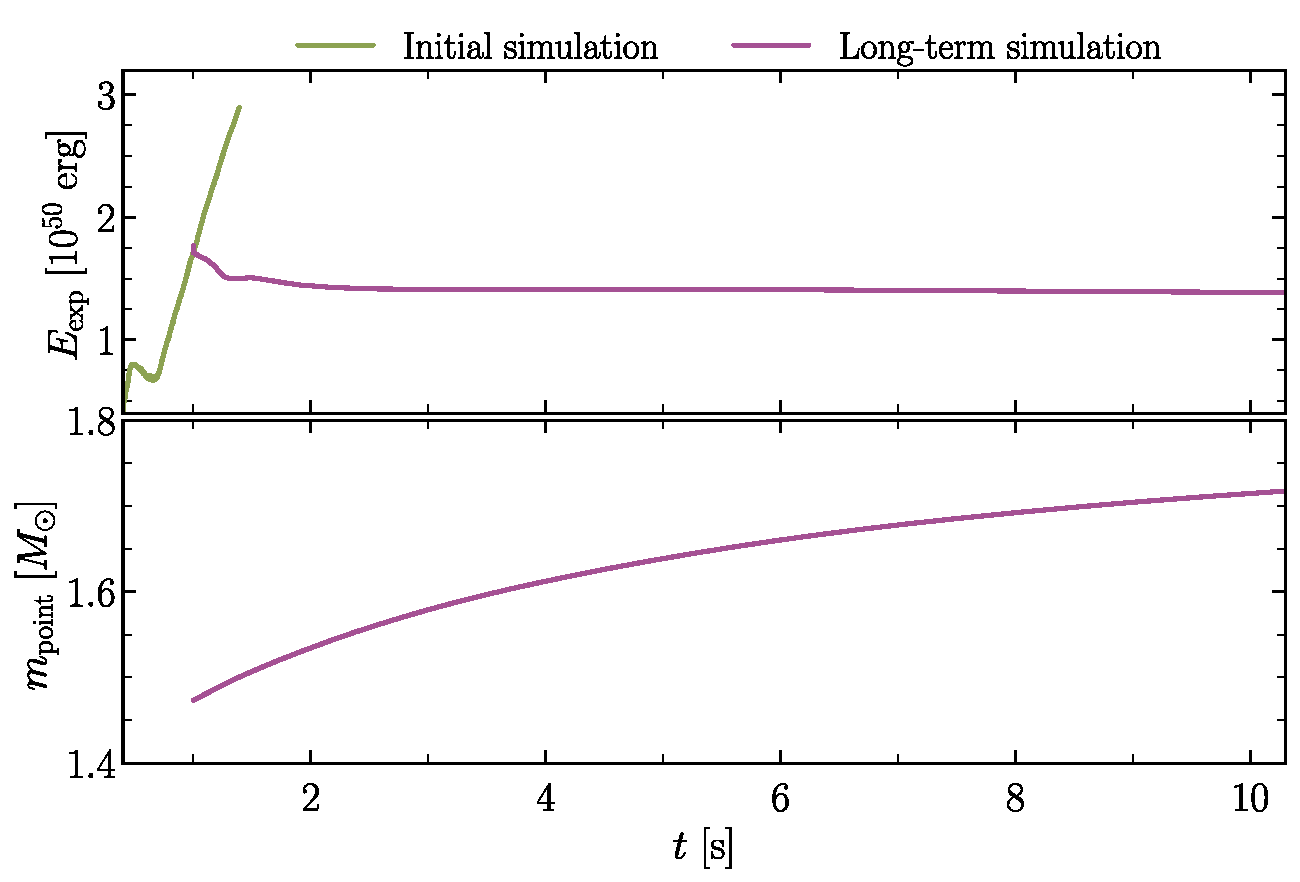
\includegraphics[width=0.9\linewidth]{figures/s12hf1p0_weak_quantities.pdf}
    \caption{Diagnostic explosion energy (top) and point mass (bottom) evolution from time of mapping at \(t_\mathrm{map} = 1.0 \units{s}\) to \(10\units{s}\) post-bounce for the s12hf1p0\_w10e8 simulation.}
    \label{fig:s12hf1p0_weak_quantities}
\end{figure}

We see that the spherical symmetry of our neutrino-driven wind clashes with the asymmetries of the initial simulation, and that if the strong wind better matches the apparent evolution of the explosion energy of the initial simulation, it results in undesirable consequences on the hydrodynamics. However, a higher heating factor can help the formation of a more spherically symmetric ejecta, rendering our neutrino wind possibly more accurate. \Cref{fig:s12hf1p5_og}, showing slices of the initial s12hf1p5 simulation at time of mapping, demonstrate this effect, as the material is more easily driven outward with very few accretion channels onto the PNS due to the slightly larger heating factor.

\begin{figure}
    \centering
    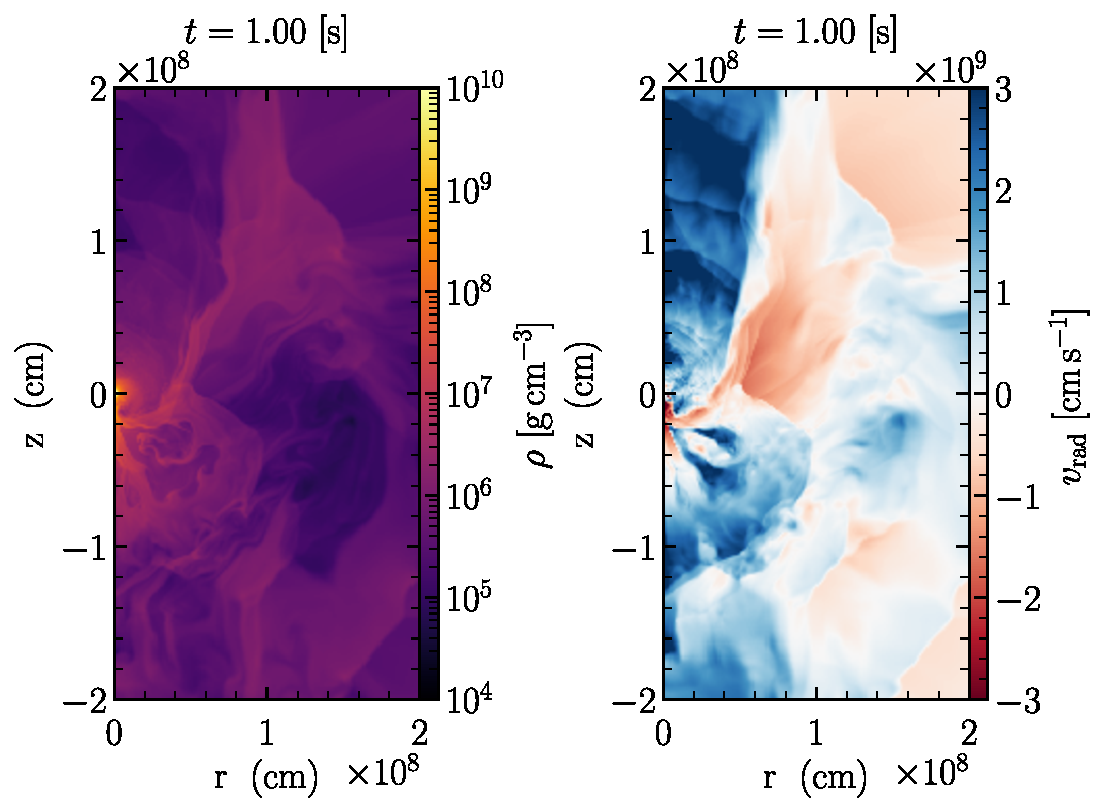
\includegraphics[width=1.0\linewidth]{figures/s12hf1p5_og.pdf}
    \caption{Slices of the initial s12hf1p5 simulation, showing density (left) and radial velocity (right) near the PNS at time of mapping.}
    \label{fig:s12hf1p5_og}
\end{figure}

The wind velocities we used for the two simulations we ran on this progenitor only differ slightly, with the weaker wind being set to \(13{,}000\units{km/s}\) and the stronger wind to \(15{,}000\units{km/s}\). However, as shown in \Cref{fig:s12hf1p5_weak_quantities,fig:s12hf1p5_strong_quantities}, this is enough for the weaker wind to keep the explosion energy mostly constant, whereas the stronger wind succeeds in injecting energy that matches with the initial simulation, without strong hydrodynamical consequences, while almost completely shutting down accretion. We also note that this progenitor initially results in a stronger explosion at moment of mapping compared with the s12hf1p0 simulations.

\begin{figure}
    \centering
    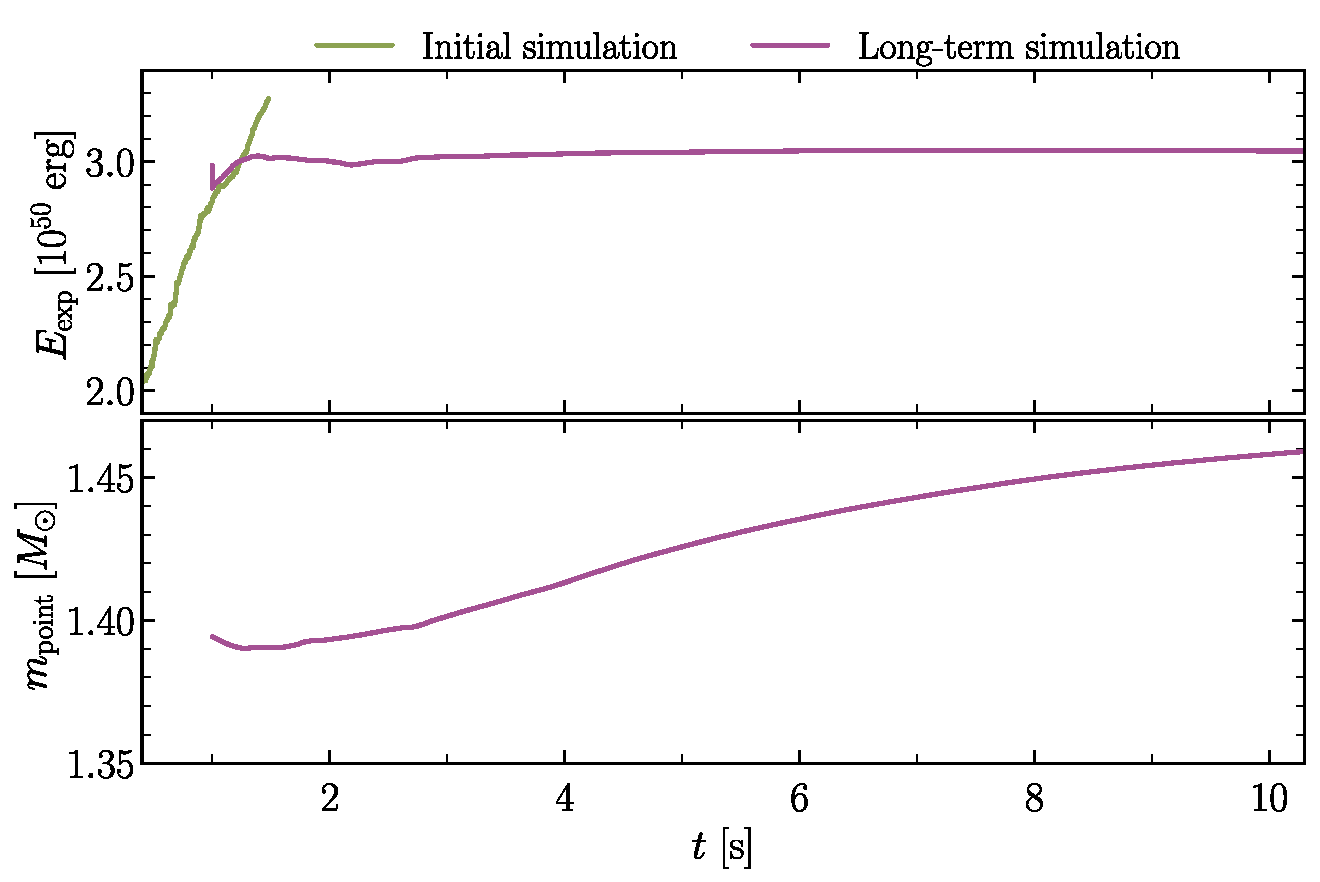
\includegraphics[width=0.9\linewidth]{figures/s12hf1p5_weak_quantities.pdf}
    \caption{Diagnostic explosion energy (top) and point mass (bottom) evolution from time of mapping at \(t_\mathrm{map} = 1.0 \units{s}\) to \(10\units{s}\) post-bounce for the s12hf1p5\_w13e8 simulation.}
    \label{fig:s12hf1p5_weak_quantities}
\end{figure}

\begin{figure}
    \centering
    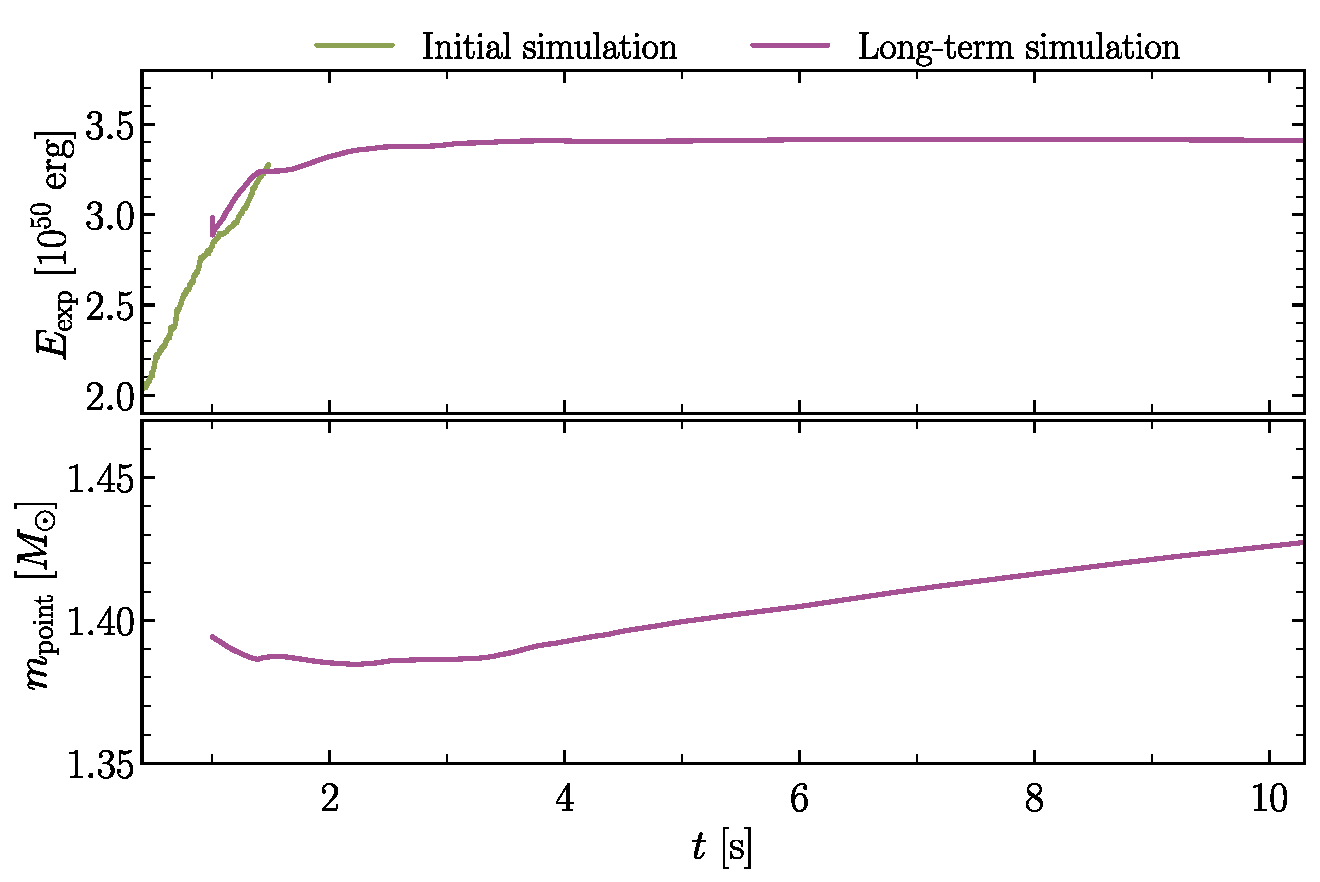
\includegraphics[width=0.9\linewidth]{figures/s12hf1p5_strong_quantities.pdf}
    \caption{Diagnostic explosion energy (top) and point mass (bottom) evolution from time of mapping at \(t_\mathrm{map} = 1.0 \units{s}\) to \(10\units{s}\) post-bounce for the s12hf1p5\_w15e8 simulation.}
    \label{fig:s12hf1p5_strong_quantities}
\end{figure}

\clearpage

We now take a look at the final simulation, that was run with a heating factor \(f_\mathrm{heat} = 2.0\), but only one wind velocity, obtained from the spherically averaged profile of the initial simulation, of \(15{,}600\units{km/s}\). Again, \Cref{fig:s12hf2p0_og} shows the state of the initial simulation at time of mapping, where almost no matter is being accreted, and we can even identify a termination shock at the south hemisphere of the simulation, about \(1.5 \cdot 10^8\units{cm}\) away from the PNS, where a neutrino-driven wind seem to have naturally started to form. Consequently, \Cref{fig:s12hf2p0_slice} shows that there are no noticeable hydrodynamical effects on the simulation due to the mapping of the inner boundary. However, the wind is weaker than in the initial simulation, and the termination shock has fallen back onto the inner boundary at \(2.0\units{s}\) post-bounce, but was enough to keep most of the surrounding material unbound, with one visible accretion channel. This can be observed on \Cref{fig:s12hf2p0_quantities}, that shows that the wind has managed to keep the explosion energy mostly constant after mapping, with only very small accretion, as indicated by the growth of the point mass.

\begin{figure}
    \centering
    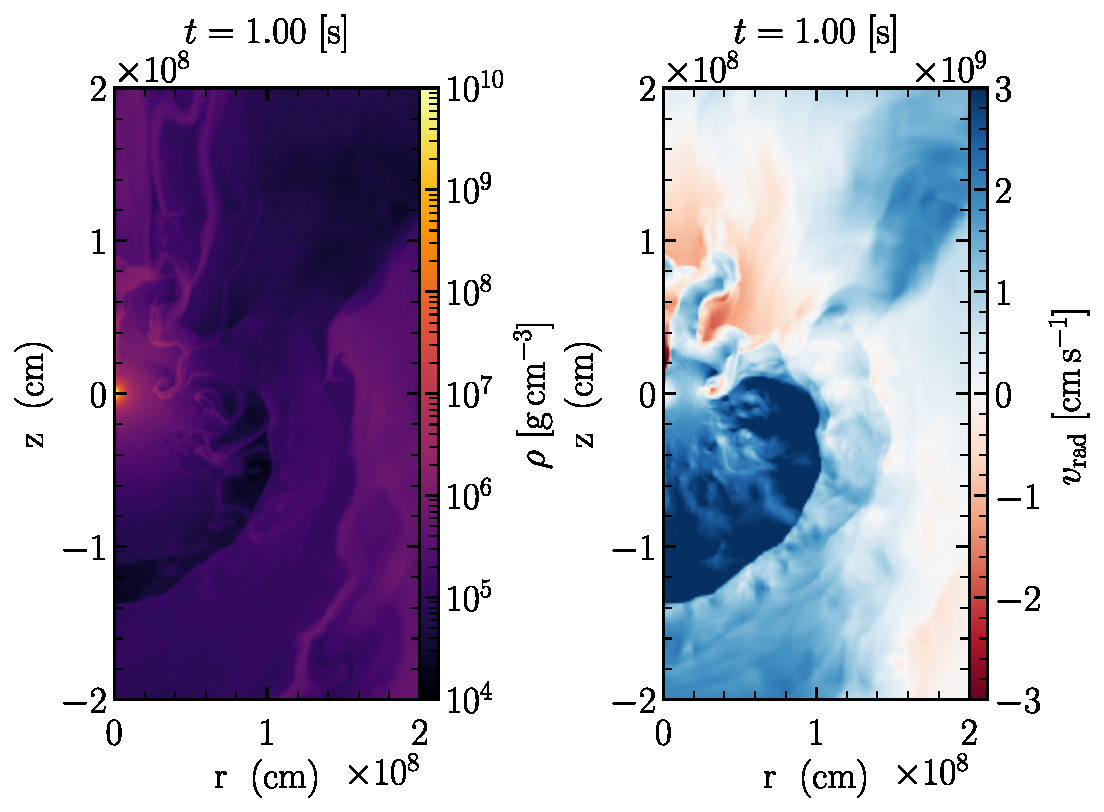
\includegraphics[width=1.0\linewidth]{figures/s12hf2p0_og.pdf}
    \caption{Slices of the initial s12hf2p0 simulation, showing density (left) and radial velocity (right) near the PNS at time of mapping.}
    \label{fig:s12hf2p0_og}
\end{figure}

\begin{figure}
    \centering
    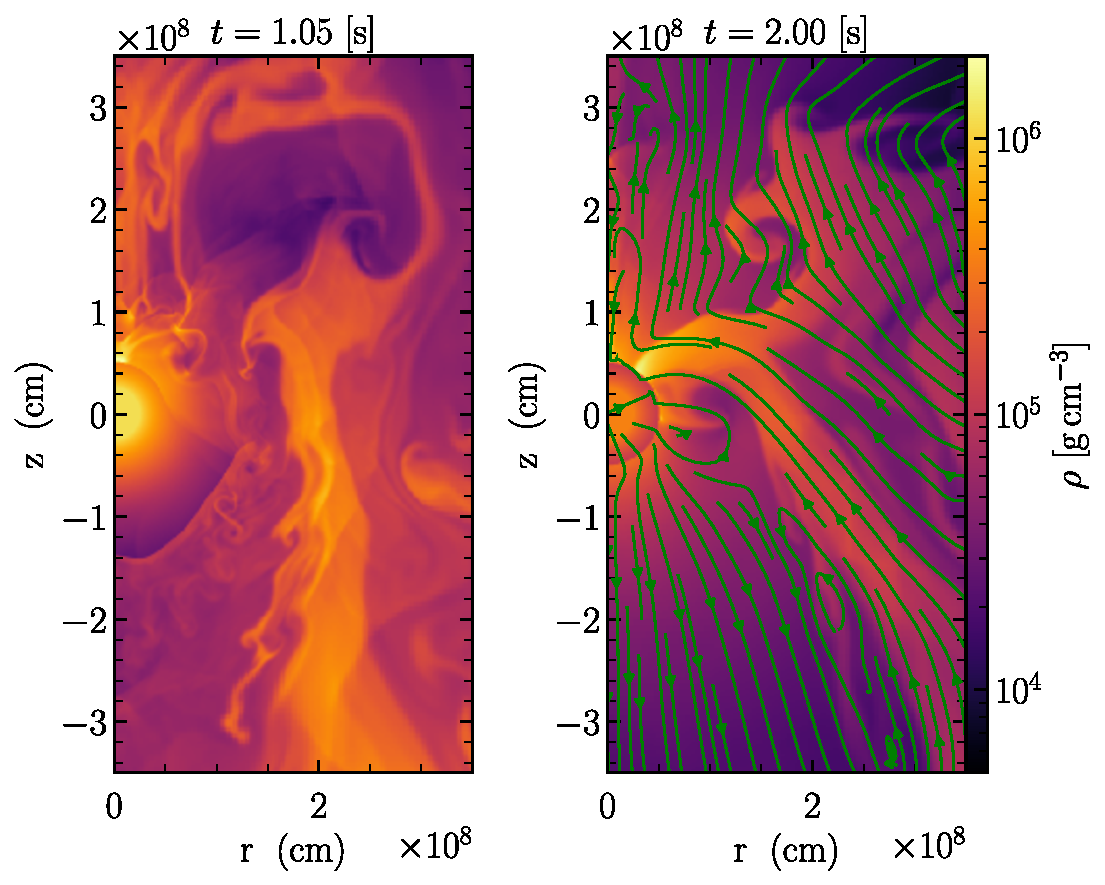
\includegraphics[width=1.0\linewidth]{figures/s12hf2p0_slice.pdf}
    \caption{Slices of the s12hf2p0 simulation at \(t=1.05\units{s}\) post-bounce (left) and \(t=2.0\units{s}\) post-bounce (right). Streamlines of the velocity field are shown in green at \(2.0\units{s}\).}
    \label{fig:s12hf2p0_slice}
\end{figure}

\begin{figure}
    \centering
    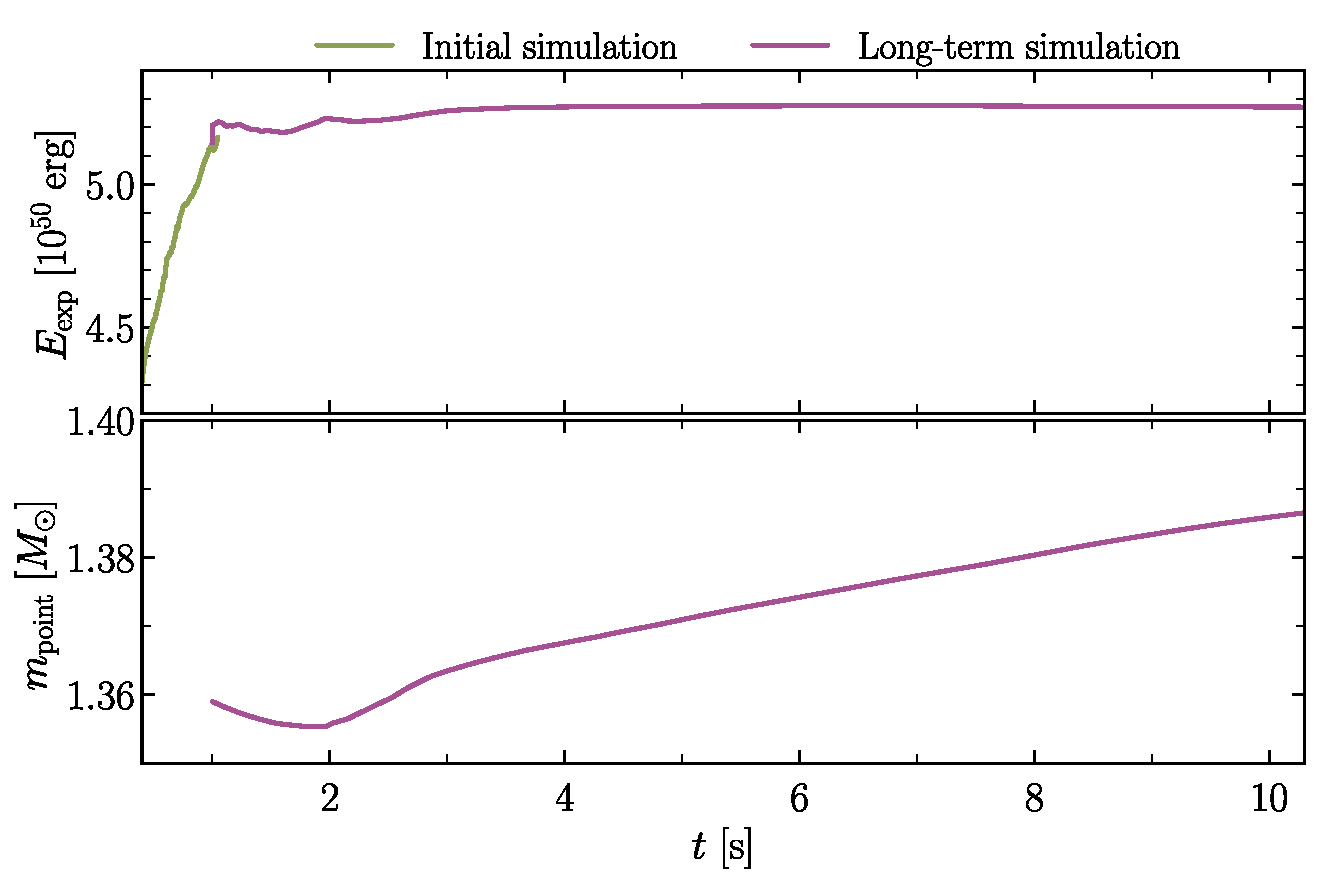
\includegraphics[width=0.9\linewidth]{figures/s12hf2p0_quantities.pdf}
    \caption{Diagnostic explosion energy (top) and point mass (bottom) evolution from time of mapping at \(t_\mathrm{map} = 1.0 \units{s}\) to \(10\units{s}\) post-bounce for the s12hf2p0 simulation.}
    \label{fig:s12hf2p0_quantities}
\end{figure}

\clearpage

\subsection{Shock breakout} \label{sec:breakout}

Finally, \Cref{fig:s12hf1p0_break} shows shock breakout from the stellar surface for the s12hf1p0\_w10e8 and s12hf1p0\_w28e8 simulations. We see that the strong wind has made the forward shock reach the surface at about \(120{,}000\units{s}\), much earlier than for the weak wind, which reaches the surface at around \(210{,}000\units{s}\).

We can in fact obtain an order-of-magnitude estimation of the time of shock breakout. Assuming that the total explosion energy is in the form of kinetic energy, we can express it as a function of the shock velocity \(v_\mathrm{sh}\) and ejecta mass \(M_\mathrm{ej}\):
\begin{equation}
    E_\mathrm{exp} = \frac{1}{2} M_\mathrm{ej} v_\mathrm{sh}^2 \punct{.}
\end{equation}

The ejecta mass being roughly equivalent to the mass of the star at moment of collapse minus the mass of the PNS, we have \(M_\mathrm{ej} \approx 9 \sunmass\) in the case of the s12hf1p0 simulation. Then, solving for the velocity, assuming it is constant, we can estimate the time required for the shock to traverse the entire star, of radius \(R\), corresponding to shock breakout:
\begin{equation}
    t_\mathrm{break} \sim \frac{R}{v_\mathrm{sh}} = \frac{R}{\sqrt{\frac{2 E_\mathrm{exp}}{M_\mathrm{ej}}}} \punct{.}
\end{equation}

Assuming the radius \(R \approx 4 \cdot 10^{13}\units{cm}\) and ejecta mass \(M_\mathrm{ej} \approx 9 \sunmass\) to be the same in both the s12hf1p0\_w10e8 and s12hf1p0\_w28e8 simulations, we can compare this quantity for the two simulations using the explosion energies shown in \Cref{fig:s12hf1p0_weak_quantities,fig:s12hf1p0_strong_quantities} to find
\begin{gather}
    t_\mathrm{break,weak} = \frac{R}{\sqrt{\frac{2E_\mathrm{exp,weak}}{M_\mathrm{ej}}}} \approx 320{,}000\units{s} \punct{,} \\
    t_\mathrm{break,strong} = \frac{R}{\sqrt{\frac{2E_\mathrm{exp,strong}}{M_\mathrm{ej}}}} \approx 196{,}000\units{s} \punct{,}
\end{gather}

where \(t_\mathrm{break,weak}\) and \(E_\mathrm{exp,weak} = 1.35 \cdot 10^{50}\units{erg}\) are the breakout time and explosion energy for the s12hf1p0\_w10e8 simulation, and \(t_\mathrm{break,strong}\) and \(E_\mathrm{exp,strong} = 3.75 \cdot 10^{50}\units{erg}\) are the breakout time and explosion energy for the s12hf1p0\_w28e8 simulation. This quantities compare with the results of the simulations, shown in \Cref{fig:s12hf1p0_break}, within a factor of 2. Furthermore, taking the ratio of these quantities gives
\begin{equation}
    \frac{t_\mathrm{break,weak}}{t_\mathrm{break,strong}} = \sqrt{\frac{E_\mathrm{exp,strong}}{E_\mathrm{exp,weak}}} \approx 1.66 \punct{.}
\end{equation}

This tells us that shock breakout must happen \(\sim1.66\) times faster with the strong wind than with the weak wind, which compares quite well with \Cref{fig:s12hf1p0_break}.

\begin{figure}[ht!]
    \centering
    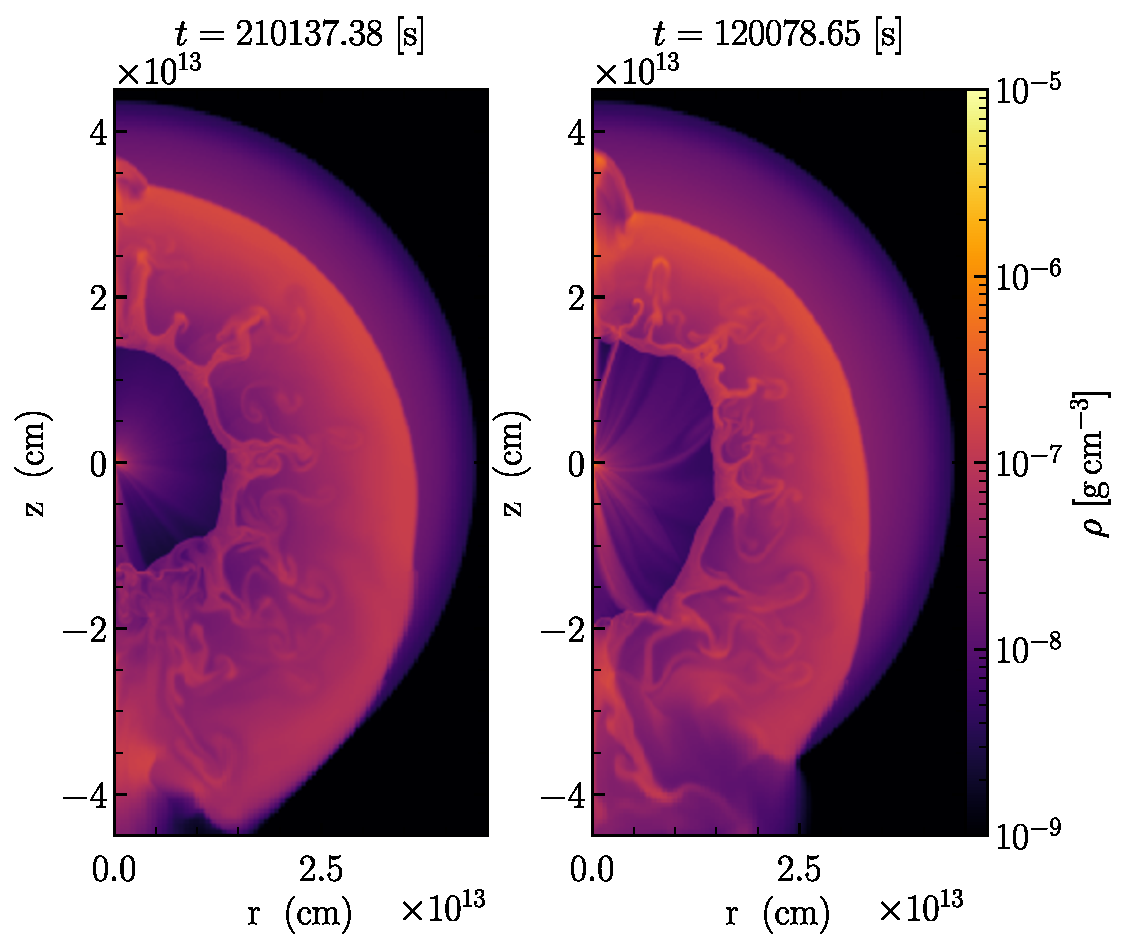
\includegraphics[width=1.0\linewidth]{figures/s12hf1p0_break.pdf}
    \caption{Density plots of the s12hf1p0\_w10e8 (left) and s12hf1p0\_w28e8 simulations (right), showing shock breakout from the stellar surface.}
    \label{fig:s12hf1p0_break}
\end{figure}


\mainchapter{Discussion}{0.6}{Your calculations are correct, but your physical insight is \flqq{} Tout à fait abominable \frqq{}.}{Albert Einstein to Georges Lemaître} \label{chap:discussion}

%----------------------------------------%
% Discussion
%----------------------------------------%

\section{Necessity of the boundary condition}

Current state-of-the-art simulation codes for CCSNe, such as \flash, are now capable of producing successful explosions with the neutrino-driven mechanism in multiple dimensions. This mechanism requires contributions from various areas of physics, including notably (magneto-)hydrodynamics, nuclear reactions, neutrino transport, general relativity, and a treatment of the equation of state of matter in both nuclear- and low-density regimes. As a result, such simulations come at a large computational cost which increases exponentially with the number of dimensions. For this reason, if 2D simulations using axisymmetry are now more common, full 3D simulations are still quite rare. Moreover, these simulations rarely extend beyond hundreds of milliseconds to a few seconds after bounce, and attention is usually given to the explosion mechanism. This computational limitation is mainly a consequence of the high resolution requirement in the central region containing the neutron star, that imposes heavy constraints on the time step required to evolve the simulation. Excising the central region from the domain is a simple yet effective solution to extend a simulation to late times at a reduced computational cost, and is the approach that we have adopted in this thesis. However, the question persists as to what should replace this region, in other words, what condition on the evolution should be put at the boundary. For example, \cite{Sandoval2021} performed simulations until late times using a diode boundary condition, similar to our description of the inflow boundary condition in \Cref{sec:bdry_in}, that exclusively allows matter to flow out of the domain. We note that in their paper, \cite{Sandoval2021} define \emph{inflow} and \emph{outflow} as matter flowing in or out of the domain, in opposition with the definition we use in this thesis, as mentioned in \Cref{sec:lt_setup}. They showed that this simple parametrisation can give valuable insights on the evolution of the initial ejecta, in particular the formation of metal-rich bullets from Rayleigh-Taylor instabilities at the shock front, and on the final morphology of the explosion. In contrast, \cite{Stockinger2020} and \cite{Wongwathanarat2015} have performed similar simulations using an outflow boundary condition mimicking the behaviour of a spherical neutrino-driven wind around the central engine, and is the description that we have based our inner boundary condition on, as described in \Cref{sec:bdry_out}. We have further explored the use of this boundary condition and analysed its effects on the simulation by modifying parameters such as the wind velocity. Also, our boundary condition exhibits an interesting property in that it evolves the cells within the inner region, thus allowing accretion onto the boundary.

\section{Validity \& Self-consistency}

Clearly, we cannot achieve self-consistency with an inner boundary condition, and the resulting simulation is bound to be an approximation. Parts of the explosion, such as the forward shock, are less affected by the introduction of an inner boundary condition, and can still provide relevant observable quantities on the late time evolution of the supernova. On the contrary, the impact on the more central regions, up to the reverse shock, and on the estimation of the nucleosynthetic yields from the inner ejecta can become non-negligible. In order to achieve long-term simulations that are as accurate as possible, a simple but realistic parametrisation of the inner boundary is required.

An inflow condition is perhaps the most simple parametrisation, but is not very suited unless the central engine is a black hole, as it causes most of the inner ejecta behind the reverse shock to fall back and accrete onto the central region. In the presence of a neutron star central engine, we require a more appropriate parametrisation capable of supporting this material from below, making a neutrino-driven wind a more reasonable choice. Furthermore, the neutrino-driven wind is expected to form due to the emission of neutrinos by the PNS, and this behaviour has been observed in several recent multidimensional simulations of CCSNe \citep{Witt2021,Navo2023,Wang2023}. \cite{Wang2023} show that the wind is a common feature of long-term CCSN simulation and demonstrate their existence. Moreover, they show that this wind can carry 10\%-20\% of the explosion energy.

\section{Main results \& limitations}

\subsection{Dimensionality}

The neutrino-driven wind is usually defined as an isotropic, spherically symmetric neutrino-heated outflow originating from the surface of the PNS. This is a standard feature of exploding 1D simulations, due to the inherent spherical symmetry of the problem, but is less well defined in multiple dimensions. As we have seen in \Cref{sec:results_2d}, our 2D simulations show very aspherical combinations of downflows and outflows in the central region surrounding the PNS before mapping. Channels of accretion can be beneficial as they boost the neutrino luminosities which, in turn, can power strong outflows in the directions that are not obstructed by infalling material. We have seen that this was particularly true in the case of our initial s12hf1p0 simulation, but that the s12hf1p5 and s12hf2p0 simulations more easily drive material out before mapping due to the higher neutrino heating efficiencies. In their paper, \cite{Wang2023} emphasise that the wind is not required to be spherical, but can have various morphologies shaped by the interaction with the surrounding material, from a concentrated, cone-like region to more spread-out channels of ejection. Our spherical neutrino wind approximation is therefore very limited and should be reconsidered in multiple dimensions to better fit the conditions from the initial simulation.

\subsection{Wind velocity}

We have found that the aspherical wind forming in the 2D simulations before mapping complicates the choice of wind velocity at the inner boundary. The simulations show that typical values of the wind velocity range from \(10{,}000\units{km/s}\) to \(40{,}000\units{km/s}\), thus we have run multiple simulations with velocities in this range. We have seen that this choice influences multiple aspects of the simulation.

\begin{description}
    \item[Diagnostic explosion energy] The wind velocity influences significantly the evolution of the diagnostic explosion energy during the first few seconds after mapping. A wind too weak, such as in our s12hf1p0\_w10e8 simulation, results in an immediate drop in explosion energy, analogous to that observed in the case where the PNS collapses and a black hole forms, whereas a much stronger wind, such as in the cases of the s12hf1p0\_w28e8 and s12hf1p5\_w15e8 simulations, better reproduces the continued rise in explosion energy, as observed in the initial simulation for a few \(100\units{ms}\) after mapping, and reaches an asymptotic value within \(\sim8\units{s}\) after bounce. However, we have seen that s12hf2p0 was able to keep a nearly constant explosion energy with a relatively weak wind. This is because the higher heating factor rendered the central region more prone to hosting our boundary condition at time of mapping, with already very little accretion and a neutrino wind forming in the south hemisphere as indicated by the presence of a termination shock.

    \item[Accretion] In the same way, and as can be expected, we have seen that stronger winds limit the amount of accretion onto the inner boundary. However, the wind weakens rapidly within the first \(\sim10\units{s}\) as the density prescribed at the inner boundary drops, becoming less capable of accelerating material outwards and counteracting accretion.

    \item[Hydrodynamics] Lastly, we have seen in the case of our s12hf1p0\_w28e8 simulation that the strong wind velocity and the very aspherical conditions at mapping cause a shock to be launched from the inner boundary, interfering with the hydrodynamical evolution of the simulation. This shock propagated at supersonic speed and reached the forward shock, perturbing the explosion. However, as we have shown in \Cref{sec:breakout}, the explosion energy can be linked to the shock breakout time, therefore the neutrino-driven wind inevitably leads to a change in the hydrodynamics as it injects more or less energy into the explosion, affecting the shock velocity. This is however not unwanted as the objective is to match as closely as possible the expected behaviour of the simulation if it was simulated self-consistently, without a boundary condition.
\end{description}

\section{Possible improvements}

Possibly the most important of these results is the impact on the hydrodynamics. This directly sets an upper limit on the wind velocity that we can prescribe if it causes the formation of a shock that interferes significantly with the shape of the forward shock. A prescription capable of preventing excess accretion while having little impact on the overall hydrodynamics and, consequently, the explosion energy, such as is the case in our s12hf2p0 simulation, is more desirable. In the case of s12hf2p0, however, most of the accretion was already shut off at moment of mapping due to the enhanced neutrino heating efficiency. A possible solution would therefore be to map at a later time of the simulation, such as \(2\text{-}3\units{s}\) after bounce, when accretion naturally slows down. However, this involves an additional, potentially non-negligible computational cost, which would be particularly limiting in the case of 3D simulations. There is no guarantee that the conditions at the inner boundary would become more favourable later. For example, \cite{Witt2021} show that most of their 2D simulations do not develop steady neutrino winds and that significant downflows can last for over \(3\units{s}\) after bounce. The simulations that do form a neutrino wind only do so after \(3\text{-}6\units{s}\) post-bounce.

We have also discussed that the neutrino wind can adopt various shapes in the case of multidimensional simulations. Our spherically symmetric neutrino wind is perhaps too simplistic, and a more complex, multidimensional boundary condition could be more appropriate. This multidimensional boundary condition could then integrate regions of accretion and ejection of material that would better match the conditions at time of mapping. The boundary could then, for example, smoothly shut off the accretion and restore its spherically symmetric character using a time dependent prescription on the velocity. Such a boundary condition needs to be carefully modelled, but has more potential at adapting to highly progenitor dependent conditions. It is not clear however what the dependence of the neutrino wind on the progenitor star is. \cite{Bollig2021} did not observe the development of a spherical neutrino wind in their 3D simulation of a \(19\sunmass\) progenitor even after \(7\units{s}\) post-bounce. They argue that an isotropic wind could principally be a feature of progenitors in the low-mass end of the CCSN range with low core compactness, as these progenitors only produce low-energy explosions of \(0.1\text{-}0.2\units{B}\). Conversely, long-lasting accretion channels powering neutrino-heated outflows are essential to producing powerful explosions in more massive stars. Furthermore, we have performed 1D and 2D simulations, but the 3D case must be considered as well. \cite{Muller2015} compared the dynamics of the material surrounding the PNS after shock revival in 2D and 3D. They showed that 2D simulations are more prone to forming laminar flows, where the interfaces between the accretion channels and the neutrino-heated material stays stable for a longer period of time, such as can be observed in \Cref{fig:s12hf1p0_og}. Conversely, 3D simulations of the same progenitor will be affected by the Kelvin-Helmholtz instability and rapidly disrupts these interfaces, leading to more turbulent behaviours of the material. As a result, accretion may be more easily shut off in 3D simulation, facilitating the introduction of our boundary condition even at early times.

\section{Outlook}

In this thesis we have presented and discussed an inner boundary condition based on the development of a neutrino-driven wind around the PNS, but other parametrisation are possible. Moreover, certain parameters, such as rotation and magnetic fields, have not been explored at all in this work. With the final aim of linking the simulated explosion mechanism and progenitor properties to observations, performing long-term simulations with a more specific parametrisation can provide valuable insights on certain exotic supernovae and transient events. For instance, the origin of Gamma-Ray Bursts (GRBs) is not very well constrained, but most likely associated with the death of massive stars. A possible scenario is the \emph{collapsar} scenario, where a massive star undergoes a failed supernova and forms a black hole. The infalling material then forms an accretion disk around the black hole and can provide a substantial amount of energy to the supernova as well as power relativistic jets causing a GRB. Such scenario was explored by \cite{Menegazzi2024} on a \(20\sunmass\), rotating progenitor star using an inner boundary condition modelled after the disk wind, where an outflow driven by the accretion disk is forced on an angle around the equator, while material is only allowed to infall towards the central engine at the poles.

Another possible scenario associated with GRBs is the \emph{magnetar} scenario. Magnetars are highly magnetised neutron stars with magnetic fields of the order of \(10^{14}\text{-}10^{15}\units{G}\), and could represent \(\sim10\%\) of newly born neutron stars \citep{Kouveliotou1998}. It is argued that fast-spinning neutron stars, with periods of a few milliseconds, could achieve magnetar fields. The two properties of fast rotation and strong magnetic fields would naturally lead to strong relativistic jets powering GRBs. Hypernovae, very powerful supernovae with explosion energies near \(\sim10\units{B}\), could be the birth place of these fast rotators, which in turn would be powered by tapping in the spin kinetic energy of the proto-magnetar \citep{Burrows2021}. It was shown that magnetar central engines can deposit a significant amount of energy into the supernova and substantially brighten the light curve \citep{Kasen2010}. An inner boundary condition modelled after the spin-down of a magnetar central engine could provide valuable information on such events as GRBs, hypernovae and Super-Luminous Supernovae (SLSNe).


\mainchapter{Epilogue}{0.6}{I suffered often, I was wrong sometimes, but I loved.\\It is I who have lived and not an illusion created by my pride and my boredom.}{Alfred de Musset, \\\textit{On ne badine pas avec l'amour}} \label{chap:outro}
%{0.35}{Points to Ponder: ...}{Evan O'Connor}

%----------------------------------------%
% Epilogue
%----------------------------------------%

Performing long-term simulations of core-collapse supernovae self-consistently from first principles is too computationally expensive. A common approach to this problem is to use an inner boundary condition to relax the time step constraint imposed on the simulation by the central cells, near and inside the proto-neutron star. However, little work has been done in this direction and often consist of coarse approximations that do not model well the conditions at the inner boundary.

We have implemented into the state-of-the-art \flash\ simulation code a new inner boundary condition modelling an isotropic neutrino-driven wind forming near the proto-neutron star, following the description of \cite{Wongwathanarat2015} and \cite{Stockinger2020}. We have performed 1D and 2D simulations until shock breakout and analysed the impact of the boundary condition and its parametrisation on the evolution. We have found that the neutrino wind has a non-negligible influence on the inner ejecta and the evolution of the diagnostic explosion energy during the first few seconds after bounce, corresponding to the cooling of the PNS. However, the mapping of the inner boundary can significantly interfere with the hydrodynamics in the presence of strong, asymmetrical downflows and outflows in the central region. In particular, the results from our 2D simulations indicate that our time of mapping, at \(1\units{s}\) after bounce, was too early, as strong and aspherical accretion channels are still active at that time and complicate the introduction of our spherical neutrino wind boundary condition. Mapping at later times, when accretion has weakened and the explosion energy reaches an asymptotic value, should solve this problem. It is however uncertain how long this can take, and may represent a non-negligible computational cost. In addition, the dependence on the progenitor is also unclear, and low-mass progenitors could more easily develop a spherical wind while more massive progenitors may experience stronger and longer-lasting accretion. Consequently, we find that the assumption of a spherically symmetric neutrino wind is limiting. Moreover, \cite{Wang2023} showed the formation of aspherical neutrino winds in their 3D simulations, leading to significant injections of energy into the explosion. This challenges the isotropic wind approximation, and calls for a more complex, multidimensional modelling of our inner boundary condition.

Apart from the neutrino-driven wind, alternative parametrisation of the inner boundary can be used to explore more exotic central engines, such as magnetars and disk-driven winds forming from an accreting black hole.


\chapter*{Acknowledgements}
\addcontentsline{toc}{chapter}{Acknowledgements}

\renewcommand{\epigraphflush}{flushright}
\setlength{\epigraphwidth}{0.6\textwidth}
\myepigraph{Help will always be given [...] to those who ask for it.}{J.K. Rowling,\\\textit{Harry Potter and the Chamber of Secrets}}
\vspace{2\baselineskip}

I wish to thank my supervisor, Evan O'Connor, for giving me the opportunity to work on this project, and supervising it. I thank him for his help, his feedback during the writing of this thesis and for taking the time to answer all my questions. I also wish to thank Anders Jerkstrand for making sure that I found a project that I liked. I wish to thank Haakon Andresen, whose advice and tremendous support greatly helped me during this project, as well as outside of it. I thank Oliver Eggenberger Andersen too, for his help and for providing me with some of his Jupyter Notebooks as examples. Also from the astronomy department, I wish to thank Nariman Nik Khah for the interesting conversations at lunch, and Maria Youngman for always smiling and looking happy (that really puts you in a good mood in the morning).

Of course, I thank all my fellow Master students with which I had an amazing experience in Stockholm. In particular Keyur Vithlani, who helped me during the whole Master and even provided me with a few good references for this thesis, and Gustaf Beckman Berg for being Gustaf Beckman Berg. I also thank Alice Knutas for making circles.

Lastly, I wish to thank my family for supporting me in my studies in countless different ways. I thank my mother, Christelle, for taking the decision to home-school me, and my father, Jean-Max, for trusting me and letting me fiddle with my computer instead of doing my homework. And finally, I thank my sister, Maeva, who always pushed me forward and inspired me. I would simply not have made it here without her.

The computations were performed at NSC Tetralith provided by the National Academic Infrastructure for Supercomputing in Sweden (NAISS), partially funded by the Swedish Research Council through grant agreement no. 2022-06725.


\cleardoublepage
\phantomsection
\addcontentsline{toc}{chapter}{Bibliography}
\bibliographystyle{bibliography/aa}
\bibliography{bibliography/refs}

\cleardoublepage
\hbox{}
\thispagestyle{empty}
\clearpage
\thispagestyle{empty}

\begin{figure}
    \centering
    
\includegraphics[width=0.1\textwidth]{standalone/cat.pdf}
\end{figure}

\end{document}
